%%
% The BIThesis Template for Bachelor Graduation Thesis
%
% 北京理工大学毕业设计(论文) —— 使用 XeLaTeX 编译
%
% Copyright 2021-2022 BITNP
%
% This work may be distributed and/or modified under the
% conditions of the LaTeX Project Public License, either version 1.3
% of this license or (at your option) any later version.
% The latest version of this license is in
%   http://www.latex-project.org/lppl.txt
% and version 1.3 or later is part of all distributions of LaTeX
% version 2005/12/01 or later.
%
% This work has the LPPL maintenance status `maintained'.
%
% The Current Maintainer of this work is Feng Kaiyu.
%
% Compile with: xelatex -> biber -> xelatex -> xelatex

% 开启盲审格式 blindPeerReview=true (如:[type=bachelor,blindPeerReview=true])

% \documentclass[type=bachelor,blindPeerReview=true]{bithesis}
\documentclass[type=bachelor]{bithesis}

\BITSetup{
  cover = {
    % 在封面中载入有「北京理工大学」字样的图片,如无必要请勿改动。
    headerImage = images/header.png,
    % 在封面标题中使用思源黑体,使用此选项可以保证与 Word 封面标题的字体一致。
    xiheiFont = STXIHEI.TTF,
    %% 使用以下参数来自定义封面日期
    % date = 2022年6月,
  },
  info = {
    % 想要删除某项封面信息,直接删除该项即可。
    % 想要让某项封面信息留空(但是保留下划线),请设置为空字符串。
    % 如需要换行,则用 “\\” 符号分割。
    title = 基于混合神经隐式场的多元传感融合场景地图表征,
    titleEn = {Multi-sensororial Scene Representation Learning with Hybrid Neural Implicit Fields},
    school = 计算机学院,
    major = 计算机科学与技术,
    author = 武子睿,
    studentId = 1120190773,
    supervisor = 张艳,
    keywords = {神经隐式表达; 三维重建; 自动驾驶仿真器; 多元传感信息融合},
    keywordsEn = {Neural Implicit Representations; 3D Reconstruction; Autonomous Driving Simulator; Multi-sensor Information Fusion},
    % 如果你的毕设为校外毕设,请将下面这一行语句解除注释(删除第一个百分号字符)并填写你的校外毕设导师名字
    % externalSupervisor = 左偏树,
  },
  style = {
    % 保持参考文献的缩进样式与 Word 模板一致。
    % 如果你不需要此样式,请将此行注释掉。
    bibliographyIndent = false,
  }
}

% 使用 listings 宏包进行代码块使用,并使用了预定义的样式,
% 你也可以选用自己的喜欢的其他宏包,如 minted;
% 然而由于 minted 依赖 Python 的 Pygments 库作为外部依赖,因此出于模板的简洁程度考虑,我们没有提供 minted 进行代码块书写的示例。
\usepackage{listings}
\usepackage{graphicx}
\usepackage{algorithm, algpseudocode}

\usepackage[
  backend=biber,
  style=gb7714-2015,
  gbalign=gb7714-2015,
  gbnamefmt=lowercase,
  gbpub=false,
  doi=false,
  url=false,
  eprint=false,
  isbn=false,
]{biblatex}

\usepackage{amsfonts,amsmath,amssymb,amsthm}
\usepackage{multirow, multicol}

% 参考文献引用文件位于 misc/ref.bib
\addbibresource{misc/ref.bib}
\addbibresource{misc/references.bib}

\setlength{\floatsep}{13pt plus 2pt minus 2pt}
\setlength{\textfloatsep}{20pt plus 2pt minus 2pt}
\setlength{\intextsep}{12pt plus 2pt minus 2pt}
\abovedisplayskip=12pt plus 3pt minus 9pt
\abovedisplayshortskip=0pt plus 3pt
\belowdisplayskip=12pt plus 3pt minus 9pt
\belowdisplayshortskip=7pt plus 3pt minus 4pt


\makeatletter 
  \addtolength{\@fpsep}{4pt} 
\makeatother

\usepackage{enumitem}
\setenumerate[1]{itemsep=0pt,partopsep=0pt,parsep=\parskip,topsep=5pt}
\setitemize[1]{itemsep=0pt,partopsep=0pt,parsep=\parskip,topsep=5pt}
\setdescription{itemsep=0pt,partopsep=0pt,parsep=\parskip,topsep=5pt}

% 文档开始
\begin{document}

% 标题页面:如无特殊需要,本部分无需改动
% \input{misc/0_cover.tex}
\MakeCover

% 原创性声明:如无特殊需要,本部分无需改动
% 更改为 PDF 页面插入,如需要添加内容,可考虑先用 Word 制作再覆盖 misc/1_originality.pdf
% ====== 原创性声明(PDF 格式)======
\begin{blindPeerReview}
  
\includepdf{misc/1_originality.pdf}\newpage
\end{blindPeerReview}
% ====== 原创性声明(PDF 格式)======
% ====== 原创性声明(LaTeX 格式)======
% %%
% The BIThesis Template for Bachelor Graduation Thesis
%
% 北京理工大学毕业设计(论文)原创性声明模板 —— 使用 XeLaTeX 编译
%
% Copyright 2020-2022 BITNP
%
% This work may be distributed and/or modified under the
% conditions of the LaTeX Project Public License, either version 1.3
% of this license or (at your option) any later version.
% The latest version of this license is in
%   http://www.latex-project.org/lppl.txt
% and version 1.3 or later is part of all distributions of LaTeX
% version 2005/12/01 or later.
%
% This work has the LPPL maintenance status `maintained'.
%
% The Current Maintainer of this work is Feng Kaiyu.
%
% Compile with: xelatex -> biber -> xelatex -> xelatex
%
% 如无特殊需要,本页面无需更改

\MakeOriginality

% ====== 原创性声明(LaTeX 格式)======

% 前置页面定义
\frontmatter
% 摘要:在摘要相应的 TeX 文件处进行摘要部分的撰写
%%
% The BIThesis Template for Bachelor Graduation Thesis
%
% 北京理工大学毕业设计(论文)中英文摘要 —— 使用 XeLaTeX 编译
%
% Copyright 2020-2022 BITNP
%
% This work may be distributed and/or modified under the
% conditions of the LaTeX Project Public License, either version 1.3
% of this license or (at your option) any later version.
% The latest version of this license is in
%   http://www.latex-project.org/lppl.txt
% and version 1.3 or later is part of all distributions of LaTeX
% version 2005/12/01 or later.
%
% This work has the LPPL maintenance status `maintained'.
%
% The Current Maintainer of this work is Feng Kaiyu.

% 中英文摘要章节
\begin{abstract}
% 中文摘要正文从这里开始
本文……。

\textcolor{blue}{摘要正文选用模板中的样式所定义的“正文”,每段落首行缩进 2 个字符;或者手动设置成每段落首行缩进 2 个汉字,字体:宋体,字号:小四,行距:固定值 22 磅,间距:段前、段后均为 0 行。阅后删除此段。}

\textcolor{blue}{摘要是一篇具有独立性和完整性的短文,应概括而扼要地反映出本论文的主要内容。包括研究目的、研究方法、研究结果和结论等,特别要突出研究结果和结论。中文摘要力求语言精炼准确,本科生毕业设计(论文)摘要建议 300-500 字。摘要中不可出现参考文献、图、表、化学结构式、非公知公用的符号和术语。英文摘要与中文摘要的内容应一致。阅后删除此段。}

\end{abstract}

% 英文摘要章节
\begin{abstractEn}
% 英文摘要正文从这里开始
In order to study……

\textcolor{blue}{Abstract 正文设置成每段落首行缩进 2 字符,字体:Times New Roman,字号:小四,行距:固定值 22 磅,间距:段前、段后均为 0 行。阅后删除此段。}
\end{abstractEn}


\MakeTOC

% 正文开始
\mainmatter

% 第一章
%%
% The BIThesis Template for Bachelor Graduation Thesis
%
% 北京理工大学毕业设计(论文)第一章节 —— 使用 XeLaTeX 编译
%
% Copyright 2020-2022 BITNP
%
% This work may be distributed and/or modified under the
% conditions of the LaTeX Project Public License, either version 1.3
% of this license or (at your option) any later version.
% The latest version of this license is in
%   http://www.latex-project.org/lppl.txt
% and version 1.3 or later is part of all distributions of LaTeX
% version 2005/12/01 or later.
%
% This work has the LPPL maintenance status `maintained'.
%
% The Current Maintainer of this work is Feng Kaiyu.
%
% 第一章节

\chapter{绪论}

\section{研究背景}
三维场景地图的重建对三维计算机视觉、机器人学等领域有着重大意义,《“十四五”机器人产业发展规划》中指出,“机器人+”应用行动应该在汽车领域着力开发和推广。近年来, 国内外涌现了一大批优秀的自动驾驶企业,希望通过自动驾驶算法,在保证驾驶安全的前提下,逐步用计算机算法代替驾驶员来进行决策。然而,自动驾驶算法的落地过程并不是一帆风顺的,随着越来越多自动驾驶车辆由于算法缺陷导致的交通事故的出现,自动驾驶算法安全性愈发得到科研界、产业界的关注。为了不断提高自动驾驶算法安全性,研究者致力于实现从真实(Real)到仿真(Sim),再到真实的数据闭环,这一过程被称为Real2Sim2Real:
\begin{enumerate}
    \item \textbf{Real2Sim:} 从真实感知数据中进行三维重建,并建立仿真化环境,在仿真场景中不断迭代自动驾驶算法;
    \item \textbf{Sim2Real:}再将迭代后的算法重新部署到真实自动驾驶车辆中,而真实车辆运行过程中采集到的新数据可以被增补到仿真环境中,建立更富有真实感的仿真驾驶环境。
\end{enumerate}

而为了实现这一目的,则需要保证从Real2Sim得到的仿真三维重建场景可以做到与真实观测结果相匹配,否则从仿真器中迭代训练的自动驾驶算法很容易受到领域偏差的影响,从而在真实道路环境中产生安全隐患。

因此,本文着力于解决Real2Sim2Real的第一环,即Real2Sim的场景地图三维重建。本文发现在现存的视觉三维重建方法通常存在一系列问题。
由于自动驾驶算法通常需要多元传感信息的输入(如RGB图片、LiDAR等深度感知信息、GPS位置信息等),为了构建具有真实感的自动驾驶仿真器,需要在重建的仿真三维地图中,为自动驾驶算法Agent提供真实感的图片渲染、精确的深度信息和准确的位置信息。
因此对于一个应用于仿真场景搭建的三维重建方法,最受关注的几个性能指标包括渲染的RGB图片是否真实,以及其对地图中物体的几何结构表示的准确性。

为了真正实现从实际道路驾驶数据中重建一个精准的三维世界, 本课题中将解决以下几个重要的科研问题:
\begin{enumerate}
    \item \textbf{混合隐式场景表示学习}:现有三维重建方法大多通过显式建模场景中的几何单元(如“点”,“网格”等)实现对三维物理世界的感知,然而这类方法通常无法满足Real2Sim自动驾驶仿真器对于渲染、几何的共同要求。本文将结合近年来广受关注的隐式场景表示,探索“在理想情况下,通过多元传感器信息进行三维重建”这一问题,也即探索三维场景地图表征的极限能力。

    现有三维重建方法中使用传统显式的点云、栅格地图,只能根据传感器分辨率在有限分辨率对场景进行描述,对于存储的开销较大。近年来,基于神经网络的隐式地图得到了显著的发展,这类方法通过拟合一个隐式函数来对环境的关键物理量进行表征,从而对场景进行无限分辨率的表达。典型的隐式场有神经辐射场、神经有符号距离场等。

    然而现有传统方法或单一隐式场方法不能同时建模较好的场景外观和精确的几何,从而限制了其在下游应用场景上的应用。如果使用混合的隐式表征(即混合隐式场),能够同时渲染逼真图片并且对于环境的几何形状有较为准确的表达,将会对下游重定位任务的执行、自动驾驶技术的提升等有巨大的帮助。
    
    \begin{figure}[t]
        \centering
        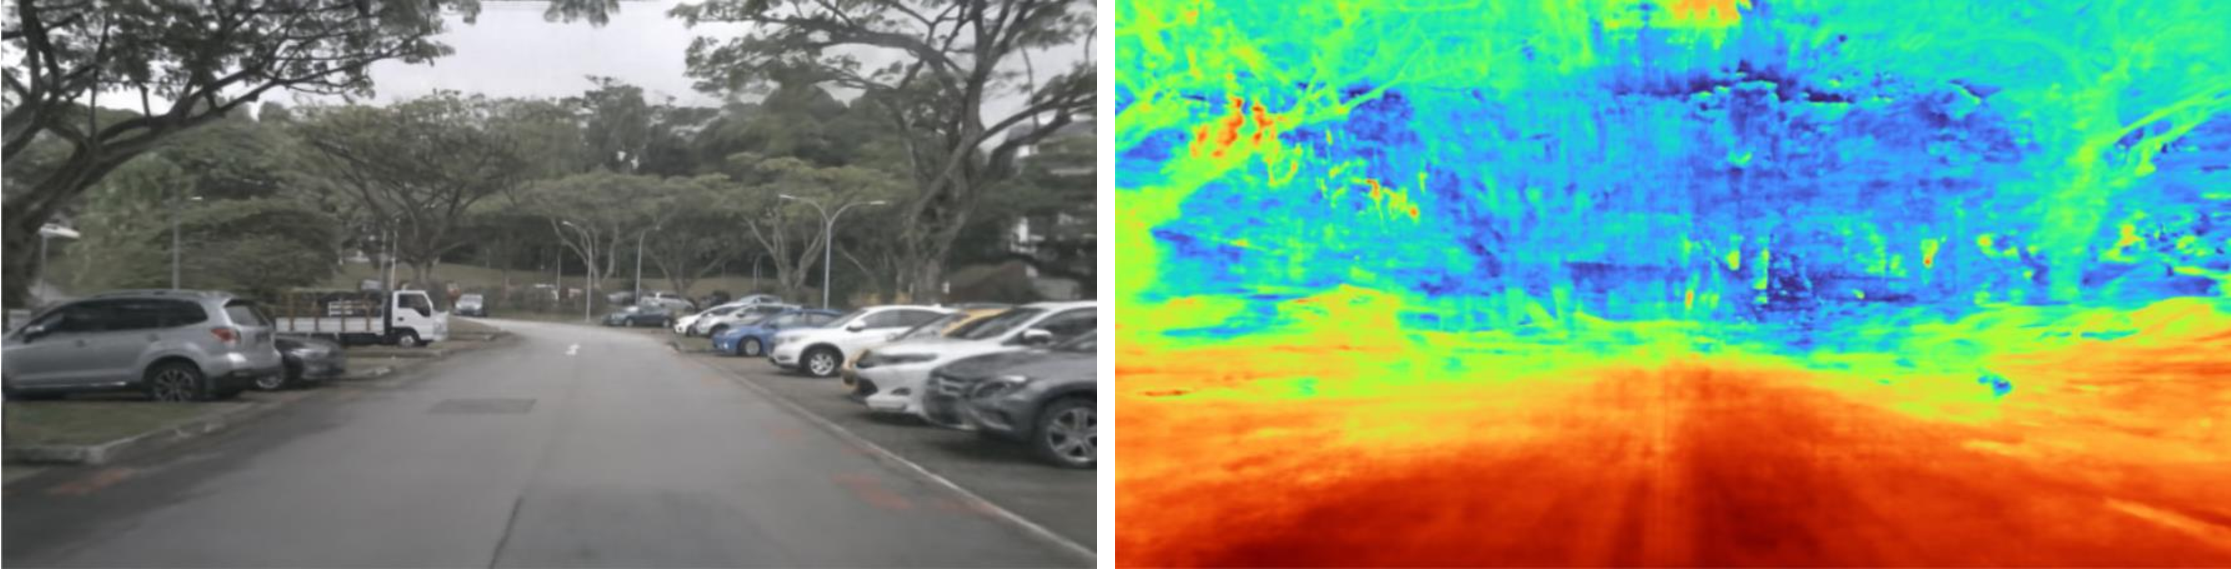
\includegraphics[width=0.9\textwidth]{undergraduate-thesis/images/RGB-D.pdf}
        \caption{左图为神经辐射场渲染的RGB图片,右图为同样位姿下渲染的深度图。可以看到辐射场对于场景外观信息建模能力较强, 但对于场景几何的学习效果较差。}
        \label{fig:rgb-d}
    \end{figure}
    
    % 除此以外,由于神经辐射场中仅用“辐射”代替物理光照模型中光的全部传播规律,因此不能用于灵活地改变环境光照
    现有混合隐式场方法尝试将距离函数映射为辐射场中用于体积积分的体密度\cite{wang_neus_2021, azinovic_neural_2022}。本文发现目前的混合隐式表征中存在诸多潜在的问题:
    \begin{itemize}
        \item 目前方法中,通常使用一个函数映射将距离值转换为体密度,本文观察到现有转换方法中存在多视角误差,将会对几何表示学习产生较大影响。
        \item 同时优化多种隐式表达本质上是一个多目标优化问题,如果不对训练过程进行约束,将会显著影响每个隐式函数的优化结果。
        \item 现有方法存在训练慢、模型大、无法泛化到大场景等问题。
    \end{itemize}
    
    如图\ref{fig:rgb-d}可见,仅从RGB图片的单一传感器输入训练神经辐射场获得的场景深度图与真实值存在较大误差。使用深度损失函数等方式融入深度感知数据,然而由于这些方法的隐式场景表达本身存在多视角误差,深度信息的引入反而会影响优化问题的进行。

    \item \textbf{面向真实自动驾驶数据的多元传感信息三维重建}:在上一个问题中,本文试图在理想状态下重建仿真场景地图,然而,要完成从真实到仿真,再从仿真到真实的数据闭环,必然要进行长时间的数据迭代,在这之中,必然会遇到退化的数据,那么如何在退化输入的情况下使得重建场景尽可能接近理想状态下的地图建模结果至关重要。在本文中,本文聚焦在真实自动驾驶数据中的两个重要问题:
    \begin{itemize}
        \item 在车端传感器框架下,通常会遇到传感器采样时间不不对齐的情况,如何在不添置昂贵的硬件设备的前提下从软件层面实现在线对齐则是一个亟待解决的问题。

        虽然现有方法可以分别在不同模态的传感信息上进行自动标定,但是他们均没有利用多元传感信息之间的共同轨迹先验信息,从而在精度上不足以支撑高保真的地图重建。
        
        \item 在真实道路环境中,可能会遇到各种不同的天气,其中以雾天为代表的散射现象对自动驾驶数据精度影响尤其显著,因为散射介质不仅影响了RGB相机的能见度,同时因为悬浮粒子对于激光的反射,会使得从激光雷达获取的深度信息不再可信。

        目前的视觉图像去雾方法虽然可以在一定程度上将带雾图片进行一定程度上的还原,但是现有方法通常局限在单视角的去雾上,从而无法利用多视角一致性信息。将一系列带雾图片输入到此类方法时,虽然处理后的每张图片看起来都是经过了去雾处理,但是原本存在于图片序列中的多视角一致性却会被破坏,从而给多视角三维重建算法带来更多挑战。
    \end{itemize}

    \item \textbf{真实动态场景仿真环境建模}:现有三维重建方法通常假设场景是恒久不变的静态场景,然而在真实道路环境中,行人、其他行驶车辆的出现显然打破了这一前提,从而给三维场景重建任务带来了巨大的挑战。虽然可以简单的通过语义模型将行人、车辆忽略,而仅仅重建静态的背景部分,然而通过这样方法获得的仿真三维场景由于动态的缺失也显然不能应用于Real2Sim2Real的数据闭环。因此如何建模场景中的动态物体也是一个重要的研究问题。
\end{enumerate}

\section{国内外研究现状}

神经辐射场(Neural Radiance Fields, NeRF)\cite{mildenhall_nerf_2020}最早被用于从已观测到的视角图片中学习场景信息,并渲染新视角下的图片,这类方法可以渲染高逼真的RGB图片。神经辐射场建立在一个简化的物理光照模型上:任意三维空间中的点均会向外散射不同颜色的光,从不同视角观察空间中的同一点的颜色可能不同,且每个点都会对其他方向传播过来的光线具有阻碍传播的作用。对三维点$P_i (x,y,z)$和观察角度$V(\theta,\phi)$,点$P_i$在角度V下观察到的颜色可以被一个五维连续隐式函数$f_{NeRF}:(x,y,z,\theta,\phi)\to (c_i,\sigma_i),c_i\in[0,255]^3,\sigma_i\in \mathbb{R}$ 建模,其中$c_i$为$P_i$散射出的RGB颜色值,而$\sigma_i$为该点的体密度。通过加权累积一条光线上所穿过点的辐射值,可以达到照片级的渲染,并且由于渲染过程的天然可微性,可以用渲染图片和观察到的图片之间的误差更新隐式函数$f_{NeRF}$。虽然神经辐射场可以精准地学习场景的视觉特征,然而仅从图片渲染误差中学习到的场景几何是缺乏约束的。因此,以神经辐射场为代表的方法在场景几何学习的深度估计等任务的精度要求上(如RMSE等指标)上的效果不足以支持Real2Sim2Real的更广泛的机器人应用。

\textbf{场景表示}:在最初的神经辐射场中,研究者使用多层感知机(Multi-layer Perceptrons, MLP)来建模隐函数$f_{NeRF}$,在MonoSDF\cite{yu_monosdf_2022}, InstantNGP\cite{muller_instant_2022}等后续工作中提出使用MLP来建模该函数关系存在训练/渲染时间过长、建模能力差和遗忘等问题,并提出使用三维空间网格代替感知机学习隐函数表征。但使用三维网格建模场景信息存在模型体积大,无法泛化到大场景的问题,因此后续工作\cite{chen_tensorf_2022, fridovich-keil_k-planes_2023, cao_hexplane_2023, reiser_merf_2023}提出使用张量分解\cite{kolda_tensor_2009}的思想将三维张量分解为多个二维矩阵,从而将场景模型的空间复杂度从$\mathcal O (L^3)$降为$\mathcal O (L^2)$。本文总结现有隐式场表示的方法如下:
\begin{itemize}
    \item \textbf{多层感知机}:使用一个带残差的多层感知机分别学习混合隐式场表征。在查询时直接将空间点信息输入网络,直接预测隐函数值。如图\ref{fig:scene-representation} (a)所示。
    \item \textbf{空间体素网格}:使用一个空间体素网格存储空间中不同区域的隐式场真值,在推理时使用三线性插值计算任意给定三维空间中点的隐式函数值。如图\ref{fig:scene-representation} (b)所示。
    \item \textbf{多分辨率体素特征网格}:将三维空间按照不同分辨率分别建立空间体素网格,在网格中存储空间几何和外观的特征,并用三线性插值和一个浅层的解码器多层感知机推理隐函数值。
    \item \textbf{二维网格}:与空间体素网格相似,该类方法将隐式场表示为多个二维矩阵,在查询任意空间点的隐函数值时将该点投影到各个二维矩阵平面中,使用双线性插值得出投影点特征,将所有二维矩阵投影点的特征进行重新整合,得到最终查询点特征。如图\ref{fig:scene-representation} (c)所示。
    \item \textbf{混合表征}:同时多种相同或不同形式的隐式场表示方法。
\end{itemize}

\begin{figure}[t]
    \centering
    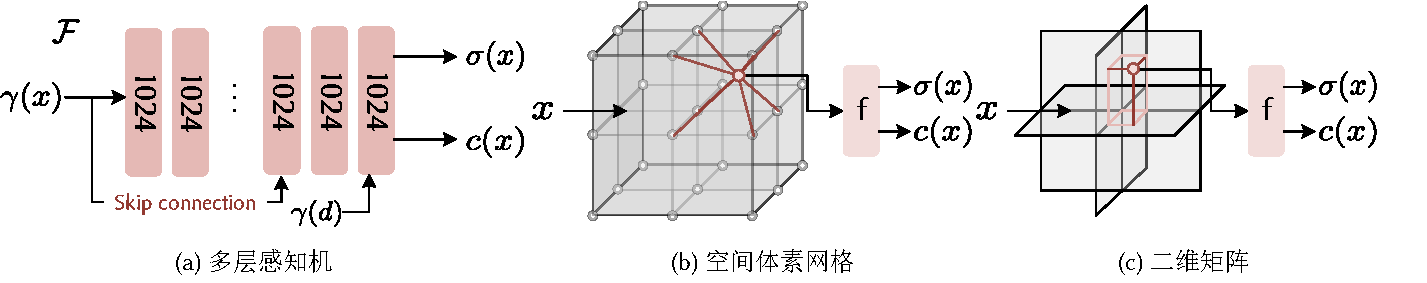
\includegraphics[width=\textwidth]{undergraduate-thesis/images/Scene Representations.pdf}
    \caption{场景表征示意图}
    \label{fig:scene-representation}
\end{figure}

\textbf{混合隐式表征}:相比神经辐射场主要通过图片中的特征学习场景的视觉信息,符号距离场(Signed Distance Fields, SDF)可以用来表达更精确的场景几何信息。在有符号距离场 $f_{SDF}:(x,y,z)→d_i$中,任意空间点$P_i$被映射到其距离最近的表面的有符号距离$d_i\in \mathbb{R}$。通过从RGB图片中抽取多视角几何对应关系,或从深度图像中获取场景几何的直接观测结果,现有方法可以通过视觉感知输入重建较为准确的场景模型。然而这类方法通常无法得到逼真的RGB渲染图片。

通过每个圆锥太体覆盖的体积的集成位置编码 (IPE) 表示,MipNeRF\cite{barron_mip-nerf_2021}有效地渲染视锥(而不是射线),从而减少了混叠的伪影现象。 NeRF++\cite{zhang_nerf_2020}分别对前景和背景表示进行建模,并分别进行采样,以应对无界 3D 场景建模的挑战。 NeRF-W\cite{martin-brualla_nerf_2021}引入了外观和瞬态编码来弥补受可变光照或瞬态遮挡物影响的弱点。 InstantNGP\cite{muller_instant_2022} 采用具有可训练特征向量的多分辨率哈希表,使 NeRF 能够学习高质量的神经图形基元。

Block-NeRF\cite{tancik_block-nerf_2022}和 Mega-NeRF\cite{turki_mega-nerf_2022} 在空间上将场景分解为单独训练的 NeRF,使场景表示能够扩展到任意大的环境。 Bungee-NeRF\cite{xiangli_bungeenerf_2022}使用多尺度数据模型,在该模型中,可以在卫星级别的截然不同的尺度上观察到图像的变化。通过引入 LiDAR 和天空建模并补偿不同的曝光,城市辐射场\cite{rematas_urban_2022}扩展了 NeRF 模型以产生令人印象深刻的 3D 表面重建并在室外环境中合成高质量的新颖视图。

此外,借助多视图立体几何\cite{deng_depth-supervised_2022} 或深度先验信息\cite{roessle_dense_2022} 的密集深度监督,NeRF 在新颖的视图合成和深度预测方面取得了惊人的成果,但难以扩展到大规模户外场景.

\textbf{相机标定:}
当前有多种 SLAM 系统通过联合估计相机参数和 3D 几何形状来重建场景。 ORB-SLAM\cite{mur-artal_orb-slam_2015}通过关联特征对应关系实时重建场景和估计相机位姿。 SfM(Structure-from-Motion,运动恢复结构) 系统\cite{schonberger_structure--motion_2016, chen_uncertainty-driven_2023} 能够同时校准内部和外部相机参数并重建场景。 相机-雷达混合SLAM\cite{kong_vmap_2023, deng_nerf-loam_2023} 对齐相机中心周围单位球体中的点和视觉特征之间的对应关系,从而提高了位姿估计精度并减少标定时间。

随着基于 NeRF 的 3D 场景重建和渲染研究的蓬勃发展,最近的工作估计了 NeRF 之上的相机参数。给定一个经过训练的 NeRF 模型,iNeRF\cite{yen-chen_inerf_2021} 能够根据观察到的图像和来自 NeRF 模型的渲染图像之间的光度损失,执行无网格、仅 RGB 的 6-DOF 位姿估计。由于 RGB 和深度的时间一致性,iMAP\cite{sucar_imap_2021} 和 NICE-SLAM\cite{zhu_nice-slam_2022} 在房间内实时进行高保真重建和位姿估计方面取得了显著成果。 Martin-Brualla 等人提出了结合 TSDF 和辐射场的混合隐式场\cite{azinovic_neural_2022},在优化相机位姿的同时提高了外观和几何形状的整体重建质量。与基于 NeRF 的方法不同,NeRFmm \cite{wang_nerf--_2022},NopeNeRF\cite{bian_nope-nerf_2022} 和 SCNeRF \cite{jeong_self-calibrating_2021} 在训练中联合优化相机位姿和内在函数。 NeRFmm\cite{wang_nerf--_2022}只能用于前向场景。 SCNeRF\cite{jeong_self-calibrating_2021} 适用于具有任意非线性失真的通用相机。两者都不能扩展到大规模场景,不适用于本文中RGB-D错配场景的设置。

\text{图像去雾:}
现有图像去雾方法大致可以分为三类:基于先验的方法、基于学习的方法和散射介质中的三维重建。
\begin{enumerate}
    \item \textbf{基于先验信息的去雾方法}。基于先验的方法依赖于物理散射模型,通过使用启发式先验来估计和去除雾霾,这些先验包括对比度最大化先验、暗通道先验、颜色衰减先验、强度框先验和非局部先验 \cite{kaiming_he_single_2009, nishino_bayesian_2012, fattal_dehazing_2015, wu_contrastive_2021}。虽然这些方法产生了视觉上逼真的结果,但所采用的先验仅限于特定场景。例如,当图像中没有天空区域时,之前的暗通道方法表现不佳\cite{kaiming_he_single_2009},因为它依赖于该区域的 RGB 值来估计大气光。此外,由于先验是在图像域中指定的,因此可能无法完全保证多视图一致性。
    \item \textbf{基于学习的去雾方法}。这种类型的早期工作\cite{cai_dehazenet_2016, fujimura_dehazing_2021, dong_multi-scale_2020, li_aod-net_2017, liu_griddehazenet_2019, qin_ffa-net_2020, qu_enhanced_2019, ren_gated_2018, ren_single_2020, zhang_densely_2018}建立在物理散射模型的基础上,并学习恢复模型中的传输图、大气光和其他变量。然而,物理散射模型对学习变量高度敏感,其中小的扰动可能导致输出图像中出现明显的伪影。最近的趋势\cite{song_vision_2022, liu_griddehazenet_2019, chen_gated_2019, deng_hardgan_2020, dong_multi-scale_2020, qin_ffa-net_2020, wu_contrastive_2021, wang_eaa-net_2021} 以端到端的方式模拟了模糊到清晰的图像转换。例如,AECR-Net \cite{wu_contrastive_2021} 在包含同一场景的成对模糊和非模糊图像的数据集上进行训练。然而,这些模型可能无法推广到分布外的数据。
    \item \textbf{散射介质三维重建}。散射介质中的 3D 重建与所提出的方法共享相似的多视图设置。他们的目标是根据从不同视点拍摄的同一朦胧场景的多张图像重建 3D 场景。然而,这些方法依赖于主动光源\cite{murez_photometric_2017, narasimhan_structured_2005, fujimura_photometric_2018, tsiotsios_backscatter_2014}、额外的感官数据,例如深度传感器或激光器\cite{caraffa_stereo_2013, li_simultaneous_2015, heide_imaging_2014, satat_towards_2018, wang_programmable_2018}。这种最近的方法\cite{fujimura_dehazing_2021, caraffa_stereo_2013, song_deep_2019, li_simultaneous_2015}依靠基于学习的技术从图像和稀疏点云中提取特征,并使用它们进行多视图立体以恢复密集的几何表示。相反,我们仅使用来自多视图的模糊图像直接恢复场景辐射度和几何形状。
\end{enumerate}

\section{本课题主要工作及主要创新点}

近年来,混合隐式表达逐渐被研究者所关注,NeuS\cite{wang_neus_2021}方法首先提出了将辐射场和距离场相结合的范式,即建立距离到体密度的映射关系,然而该方法仅考虑了单视角下的无偏和遮挡,而没用考虑多视角的一致性,此外,该方法仅从RGB图片中学习场景表示,而不能利用深度图片的信息。NeuralRGB-D\cite{azinovic_neural_2022}方法在NeuS的基础上,使用了深度图来作为额外的场景感知输入。这些现有方法简单地将辐射场和距离场表达相结合,会使得整个优化任务的难度大大提升,从而显著地影响模型的整体性能。 因此,如何将不同的隐式函数有效地结合便成为当下隐式场研究的一个核心问题。为此,本课题首先考虑在场景的密度信息和梯度信息之间建立桥梁,保证混合隐式场在多视角下的空间一致性,实现距离场和辐射场的同时协同优化,以期解决隐式场的优化问题。除此以外,目前方法在表达大场景上存在严重的泛化问题,即训练速度极慢、模型大、效果差等。在本课题中,本文使用多元传感输入(包括RGB相机、激光雷达或深度相机等),将不同模态下的传感数据进行融合,来优化混合隐式场表征。所得的混合隐式场应能被用于真实感的图像渲染、高保真深度预测和三维重建等应用场景。


\begin{figure}[t]
    \centering
    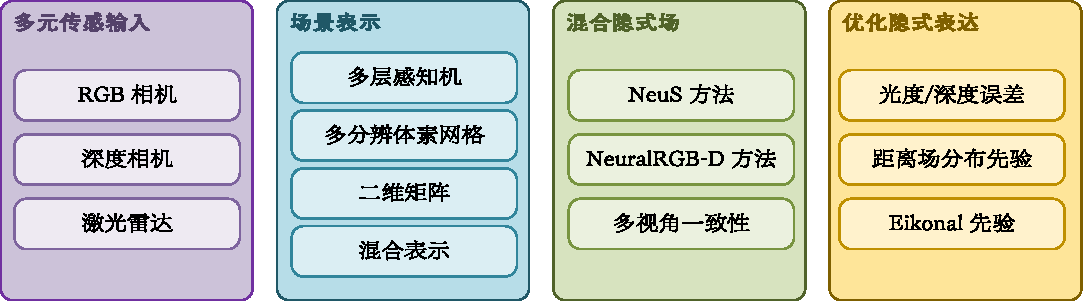
\includegraphics[width=\textwidth]{undergraduate-thesis/images/method.pdf}
    \caption{本课题中采用的技术路线}
    \label{fig:method}
\end{figure}

在此基础之上,为了解决真实自动驾驶场景中所遇到的退化输入数据,本文分别在多元传感器时间同步和雾天受散射效应影响较大两个问题上提出解决方案。为了实现对室外场景中的动态物体进行主动建模,本文通过将场景分解成场景图网络,在建模动态物体的基础上实现了对车辆行驶轨迹和外观进行编辑。

综上,本文的主要创新点和技术贡献如下:
\begin{itemize}
    \item 本文结合现有方法中不同的隐式场种类、隐式场表达,建立了基于多元传感信息输入的混合距离-辐射场,可以在场景外观颜色渲染和场景几何建模等任务超过现有方法。
    \item 从异步 RGBD 序列训练城市规模的神经辐射场,解决了现实应用中遇到的实际问题。本文在这个问题中确定了一个重要的特定领域先验:RGB-D 帧是从相同的基础轨迹中采样的。本文先将其实例化为一个新颖的时间-姿势函数,并开发一个级联隐式表示网络。
    \item 本文首次提出从带雾图像中学习神经隐式场,通过对采样点的权重进行重新配置,使得可以准确将悬浮粒子和场景的结构解耦,利用带雾图像中的隐式深度信息作为RGB图片的增补,从而实现高质量的隐式场景表示学习,并允许灵活的散射效应控制。
    \item 本文从RGB-D真实数据中学习混合隐式场景图,实现了对动态场景的理解和编辑。通过将上述技术贡献进行整合,可以实现从真实多元传感的自动驾驶数据中构建隐式自动驾驶仿真环境,从而实质性推动自动驾驶Real2Sim2Real的技术发展。
    \item 本文在公开数据集和在各种退化条件下在仿真、真实场景中采集数据上进行详尽的对比实验,验证了本课题所提出方法显著优于现有方法。
\end{itemize}

\section{本文章节安排}
本文分成六个章节,第一章(本章节)阐述本文的研究背景、意义,分析在Real2Sim2Real数据闭环的需求下为了实现Real2Sim仿真场景重建所需要解决的困难,介绍与混合隐式表达相关国内外相关工作,并最后介绍本文的主要研究工作和创新点。

第二章介绍了混合隐式场景表示这一新兴领域的相关理论和主流方法。该章首先介绍神经隐式场景表示的概念,以及场景表示模型从多层感知机逐渐演变的过程, 接着介绍用于真实感渲染的神经隐式场理论和技巧,但这一部分均只局限于单一的隐式表征,在后半部分将转而介绍同时用于精准建模场景外观和几何的混合隐式场景表示。

第三章中介绍了本文所提出的神经混合隐式场的理论框架,解决在理想情况多元传感数据输入情况下高精度建模的问题,并为后续章节提供基础。这一章中首先分析现有距离-辐射混合隐式表达中由于距离到体密度映射过程的缺陷所带来的两种误差,由这两个误差引出本文所提出的基于全方向距离场的混合隐式表达。 在此基础上,本文进而引入抗锯齿技术,以进一步提升渲染画面质量。然而这一方法只能解决理想状态下,即多元传感器均在时间上同步,且在光照、天气较为理想的情况时的高精度建模问题。

第四章介绍了本文为了实现在真实自动驾驶数据中重建高精度地图表征的一系列方法。首先,本文分析了室外数据中广泛存在但没有被解决的传感器同步问题,通过引入隐式轨迹函数(TPF),并在建图阶段持续优化,本文可以在多传感器时间异步的退化条件下获得与理想情况下相匹配的建图结果。在第四章的后半部分,本文讨论了在带雾、下雨天气等受空间散射效应影响严重的情况下,进行地图重建的问题。在这类天气下,深度传感器无法产生可信的数据,而RGB相机也会受到光线散射的影响,从而显著降低能见度。 本文通过分析散射光照模型,通过采样点重赋权、协方差损失等方法,实现与正常天气几乎一样的建图结果,并能渲染高清无雾图片。

第五章介绍了基于本文提出的混合神经隐式场构建的动态场景图。本文在前四章所介绍的方法均只能处理静态场景的建模,而为了实现Real2Sim仿真器,就需要对其中的动态物体进行单独建模,因此在这一章中介绍了使用场景图分解的方法重建动态场景的技术路线,其中被分解的每个子模型均为前文提到的混合隐式场景表征模型。在最后,该章介绍了使用训练好的场景图模型可以实现Real2Sim仿真器所需要的场景编辑能力。

第六章介绍为了验证本文中提出方法所进行的一系列分析实验和结果。在这一章中首先列出实验所使用的数据集,其中包含公开数据集和本文在真实场景下不同步和带雾两种退化场景下所构建的数据集,并介绍模型评估指标。接下来介绍本文所进行的一系列详尽的实验以验证方法有效性,除了与基线模型的对比,该章还介绍了模型中每个组件的消融实验。

本文的最后总结了全文研究工作,并展望了未来可能的可扩展研究方向。
% 在这里添加第二章、第三章……TeX 文件的引用
\chapter{文献综述}
在本章中,我们将对国内外现有相关研究工作现状进行阐述。在\ref{sec: related-work implicit scene representation learning}节中,我们将介绍以神经辐射场\cite{mildenhall_nerf_2020}为代表的使用隐式函数进行场景表示学习的主流方法。纵观神经隐式场发展的历程,人们用来学习场景外观的地图表示方法经历了从纯隐式的多层感知机地图到半隐式的体素地图、低维张量地图的变革,在该节中我们将详细介绍这一变换的过程和内在原因。在\ref{sec: related-work realistic rendering}一节中,我们将介绍人们基于神经辐射场上为了使渲染更具真实感所提出的一系列方法,包括引入无界场景压缩、前后景分割等。在\ref{sec: related-work density-distance fields}一节中,我们将介绍辐射-距离混合场景表示的方法。在该节中,我们将首先分析单纯使用辐射场同时表示场景几何和外观所带来的二义性问题,接着从采样策略、体渲染方法、多元传感信息融合以及模型优化几个角度分别介绍相关工作所使用的方法。

\section{神经隐式场景表示学习}
\label{sec: related-work implicit scene representation learning}

神经隐式场景表示,即是将三维场景的几何、外观、语义等信息抽象为一个隐式表示的函数,通过神经网络的回归能力来拟合这些隐函数。在本节中,我们将介绍使用以神经辐射场和神经符号距离场为主的神经隐式表征进行场景表示学习的主要方法。在\ref{sec: related-work MLP-based neural implicit representations}节,我们将通过神经辐射场和DeepSDF介绍使用多层感知机表示场景隐式函数的基本概念,在\ref{sec: related-work grid-based implicit representations}和\ref{sec: related-work multi-plane-based implicit representations}两节中介绍神经隐式场景表示的主干模型的改进。


\subsection{基于多层感知机的场景表示}
\label{sec: related-work MLP-based neural implicit representations}

在2020年,Ben Mildenhall等人在ECCV 2020会议上发表了神经辐射场\cite{mildenhall_nerf_2020}(NeRF)用来解决新视角合成任务(如图\ref{fig:related-work novel-view-synthesis-task}所示)。新视角合成任务输入为已知位姿的多视角图片$\{{I}_i\}^N$,希望在该场景的任意给定新视角下,渲染一张具有真实感的图片${I}_\text{target}$。所谓神经辐射场,即是在假设三维空间中任意一个三维点均在向外辐射光线并阻挡其他光线的传播这一前提下,使用一个隐式神经网络建模每个三维点的辐射量。

\begin{figure}[h]
    \centering
    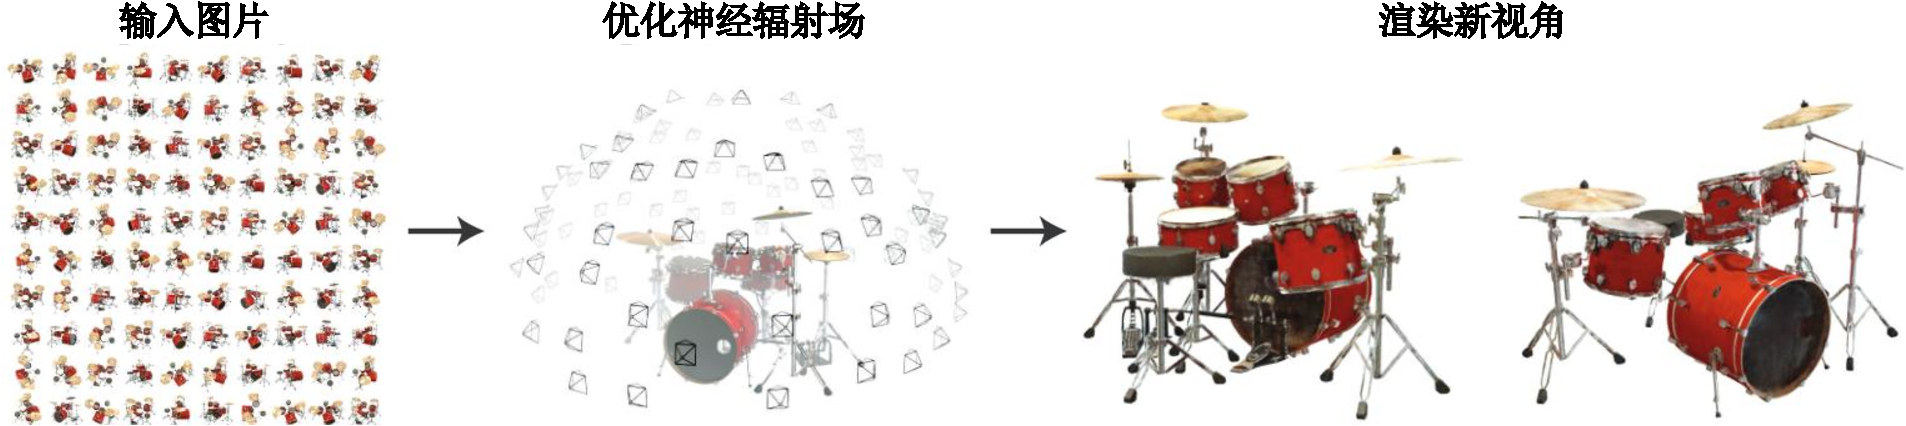
\includegraphics[width=\textwidth]{undergraduate-thesis/images/related-work/NeRF setting.pdf}
    \caption{使用神经辐射场\cite{mildenhall_nerf_2020}进行新视角合成的基本流程}
    \label{fig:related-work novel-view-synthesis-task}
\end{figure}

具体来说,辐射场可以表达为一个输入为三维欧氏空间下坐标$(x,y,z)$和观察角度$(\theta,\phi)$,输出为RGB颜色值$(R,G,B)$和体密度$\sigma$的函数,如公式\ref{eq:related-work radiance field}所示,其中$(x,y,z)\in\mathbb{R}^3, (\theta,\phi)\in[0, 2\pi]^2, \mathbf{c}=(R,G,B)\in[0,255]^3, \sigma\in\mathbb{R}^+$。RGB色值为空间点向外辐射的光的颜色,为了建模高光等物理光照现象,这个值应随观察角度的变化而变化,即$f_{\{R,G,B\}}:f_{\{R,G,B\}}(x,y,z,\theta,\phi)$,相反,体密度$\sigma$只建模三维点的物理密度,是空间点坐标的函数,与观察视角无关,即$\sigma:\sigma(x,y,z)$。根据万能近似定理\cite{hornik_multilayer_1989}(Universal Approximation Theorem),NeRF使用一个多层感知机来建模这种隐式的函数关系,即神经辐射场。
\begin{equation}
    f_\text{NeRF}: (x,y,z,\theta,\phi)\to(R,G,B,\sigma).
    \label{eq:related-work radiance field}
\end{equation}

通过累计一条光线上三维点的辐射值,我们便可以实现在任意观察视角下光线的渲染。图\ref{fig:related-work NeRF pipeline}展示了NeRF方法的总体流程:
\begin{enumerate}
    \item [a] 在观察视角发射一条光线,并在其上采样若干个三维空间点,将他们的三维欧式坐标和观察角度组成一个5元组张量$(x_i,y_i,z_i,\theta,\phi)$;
    \item [b] 通过神经辐射场,得到采样点的隐函数值$(R_i,G_i,B_i,\sigma_i)$;
    \item [c] 使用体积渲染公式,计算整条光线的渲染颜色值$\hat{c}$;
    \item [d] 将渲染值$\hat{c}$与真实观测值${c}_{gt}$比较,计算损失函数,通过反向传播优化神经网络。
    \begin{align}
    c(\mathbf{o},\mathbf{d}) &= \int_0^\infty \sigma(\mathbf{o}+t\mathbf{d})T(t)c(\mathbf{o}+t\mathbf{d},\mathbf{d})\text{d}t,\label{eq: related-work volume rendering}
    \\
    T(t) &= \exp(-\int_0^t\sigma(\mathbf{o}+t\mathbf{d})\text{d}t).\label{eq: related-work transmittance}
    \end{align}
\end{enumerate}


体渲染公式如公式\ref{eq: related-work volume rendering}所示,其中$T(t)$为累计的透光度,如公式\ref{eq: related-work transmittance}所示,通过体渲染,我们可以将三维辐射场的场景信息投影到二维的成像平面上,进行真实感的渲染。


\begin{figure}[t]
    \centering
    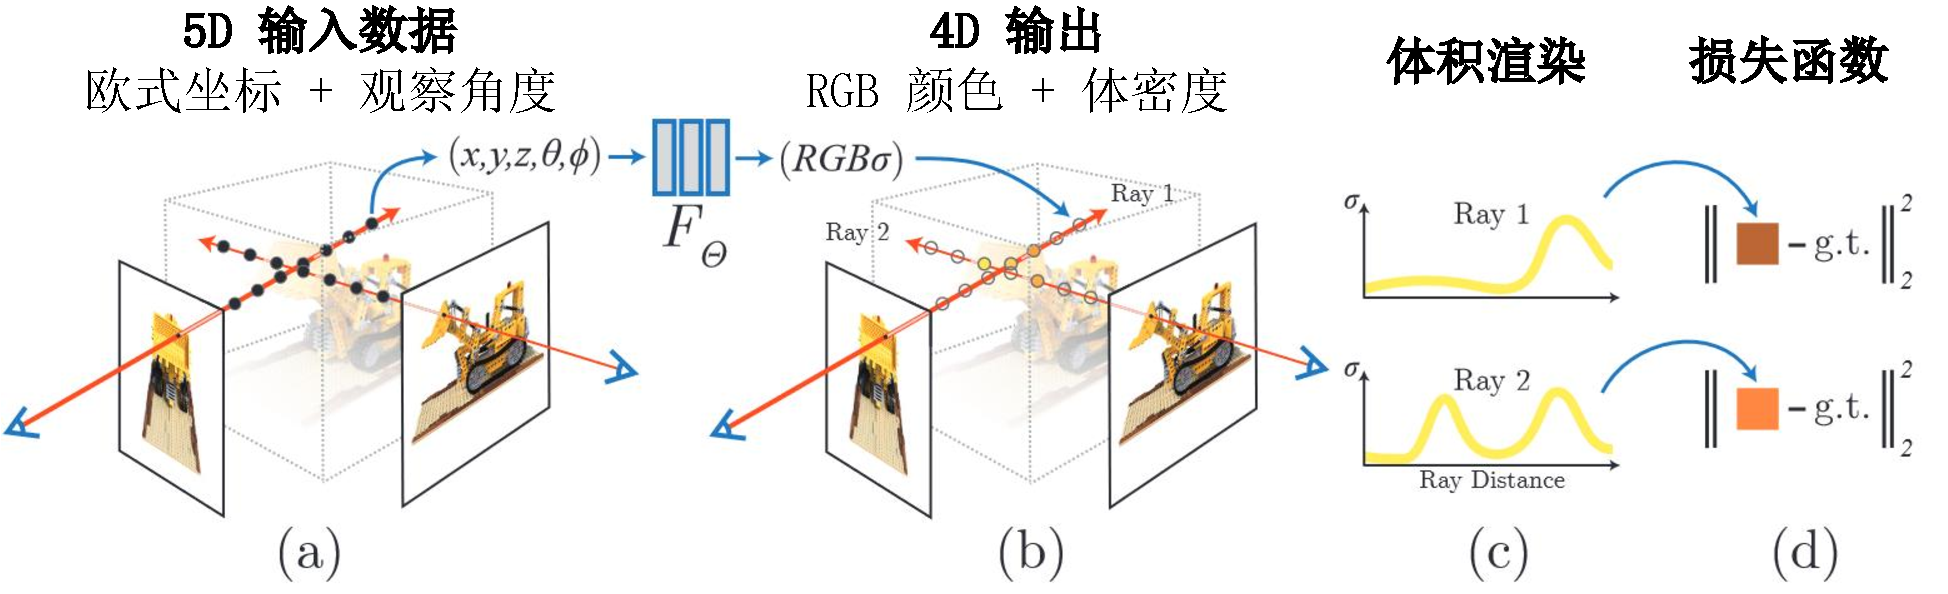
\includegraphics[width=\textwidth]{undergraduate-thesis/images/related-work/NeRF method.pdf}
    \caption{使用神经辐射场\cite{mildenhall_nerf_2020}进行训练和渲染的总体流程}
    \label{fig:related-work NeRF pipeline}
\end{figure}

\begin{figure}[ht]
    \centering
    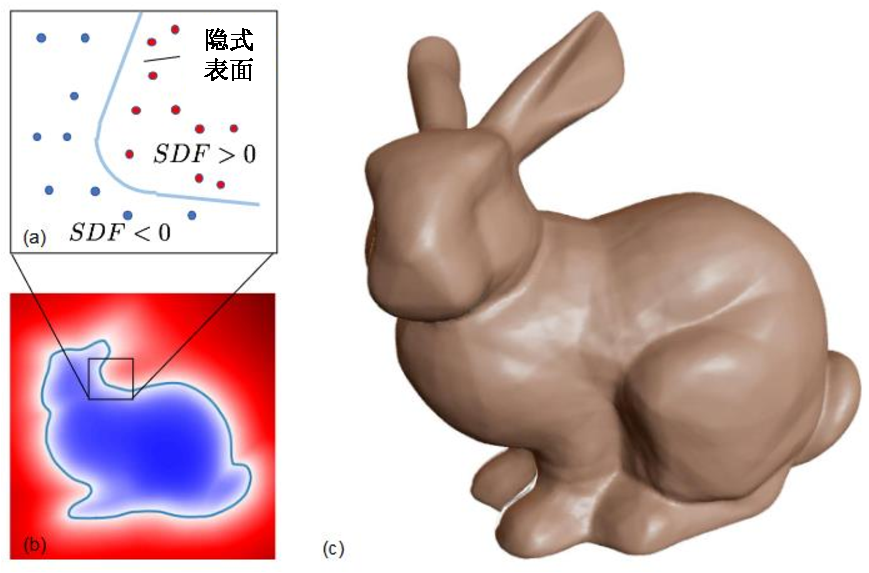
\includegraphics[width=0.7\textwidth]{undergraduate-thesis/images/related-work/SDF concept.pdf}
    \caption{符号距离场示例。图中(a)展示了由SDF函数所隐式确定的表面;(b)为符号距离场在二维的分布,蓝色区域表示SDF<0的区域,红色区域表示SDF>0的区域;(c)由三维符号距离场所确定的几何信息进一步导出的物体模型。}
    \label{fig:related-work SDF concept}
\end{figure}

除了辐射场中的函数关系,基于多层感知机的神经隐式表达也可以被用于其他任务的实现上\cite{park_deepsdf_2019, mescheder_occupancy_2019, shim_snerl_2023, zhi_-place_2021}。2019年Park等人使用多层感知机来拟合场景的三维符号距离场上。符号距离场(Signed Distance Fields, SDF)描述了场景中三维点到物体表面距离,用一个隐式函数$f_{SDF}$表示,如图\ref{fig:related-work SDF concept}所示,有向距离值的绝对值表示某三维点$\mathbf{x}(x,y,z)$到其最近表面的距离,其符号表示三维点在表面内/外,当三维点位于一个封闭曲面内部,则其$f_{SDF}(\mathbf{x}) < 0$,在表面外时$f_{SDF}(\mathbf{x}) > 0$。因此$f_{SDF}(\mathbf{x})$的零值面即为所描述的三维曲面。在DeepSDF中,作者使用一个多层感知机来拟合这一隐式函数。

\begin{figure}[ht]
    \centering
    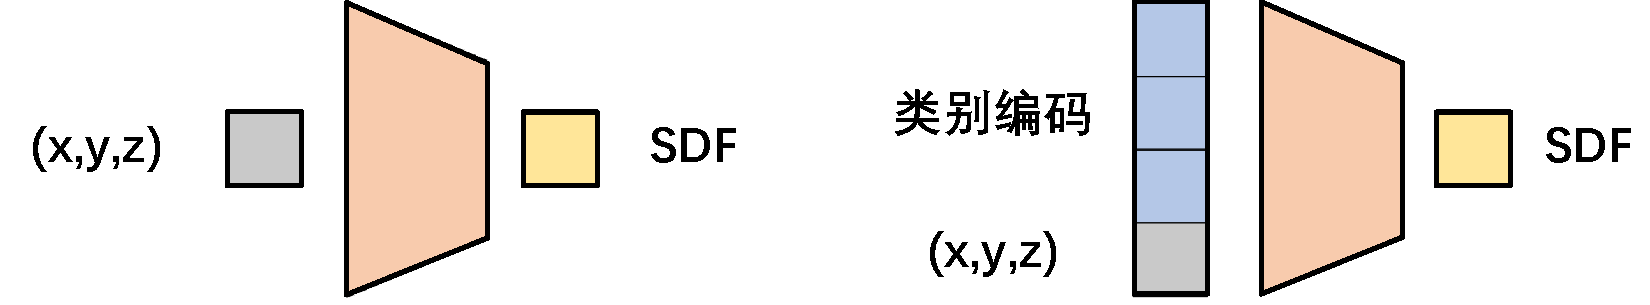
\includegraphics[width=0.8\textwidth]{undergraduate-thesis/images/related-work/deepSDF.pdf}
    \caption{DeepSDF\cite{park_deepsdf_2019}网络结构的两种形式:左侧为一般情形下直接拟合物体的SDF隐函数;右侧是带有类别编码的SDF函数。}
    \label{fig:related-work DeepSDF}
\end{figure}

不同于神经辐射场直接使用多层感知机拟合场景隐函数,DeepSDF引入类别编码,为一类具有相似形状的物体学习类别表征编码,与隐函数输入同时输入网络。这样做可以大大缩减学习同类物体SDF网络的时间,网络结构如图\ref{fig:related-work DeepSDF}所示。



\subsection{基于体素网格的场景表示}
\label{sec: related-work grid-based implicit representations}
虽然多层感知机作为一个万能函数拟合器在理论上可以无限接近场景的隐式表征函数,但这样的表示主干网络在实践中存在若干问题:
\begin{enumerate}
    \item 多层感知机的训练需要较大计算量,即使训练一个较小物体或场景的隐式函数也往往需要1$\sim$2天的训练时间才能使网络收敛,前向传播的耗时也不能满足计算机图形学实时渲染的需求;
    \item 多层感知机的训练存在遗忘问题。在一组数据上训练产生的梯度往往会影响其他数据上已经收敛的模型权重,这导致以多层感知机为主干网络的模型往往不能泛化到更大的场景上(如完整的室内场景等)。
\end{enumerate}

基于这样的观察,研究者尝试使用基于体素的场景地图主干网络。基于体素网格的场景表示可以采用一种更加直观的方式来表示3D场景,即将3D场景划分为一个网格,并在每个网格内记录它的辐射、法向量等信息。与基于多层感知机的场景表示相比,在训练和前向传播方面,基于体素网格的方法具训练时间短、效果更好等特点。

\subsubsection{传统密集体素网格地图}
早期使用体素网格地图表示的方法\cite{fridovich-keil_plenoxels_2022, kondo_vaxnerf_2021, yu_monosdf_2022}通常将三维场景离散化为一个三维空间网格,其中的每个体素(Voxel)的每个节点上存储该点上的隐式函数值。当需要查询任意一个连续空间中的三维点的隐函数值时,只需查询其周围的八个相邻节点,并使用三线性插值计算目标点的隐函数值。

我们用$\mathcal{G}_\theta$来表示一个分辨率为$R_H\times R_W\times R_D$的体素网格,则使用体素网格来作为隐式场骨干模型的方法可以写作:
\begin{equation}
    \hat{s} = \mathtt{interp}(\mathbf{x}, \mathcal{G}_\theta),
\end{equation}
其中$\hat{s}$为网络预测的隐式函数值,$\mathtt{interp}$表示三线性插值。

然而,将三维网格应用于取代原始NeRF中多层感知机的一个必然结果就是对于输入数据的限制。具体而言,原始NeRF使用物体的三维位置坐标和观察角度作为输入来建模物体的Lambertian和非Lambertian效应(即漫反射、高光等与视角相关的效应),然而使用三维网格来建模物体的辐射量则限制了输入维度仅能为三维。这种限制在某些场景下可能会对建模效果产生一定影响。

\begin{figure}[ht]
    \centering
    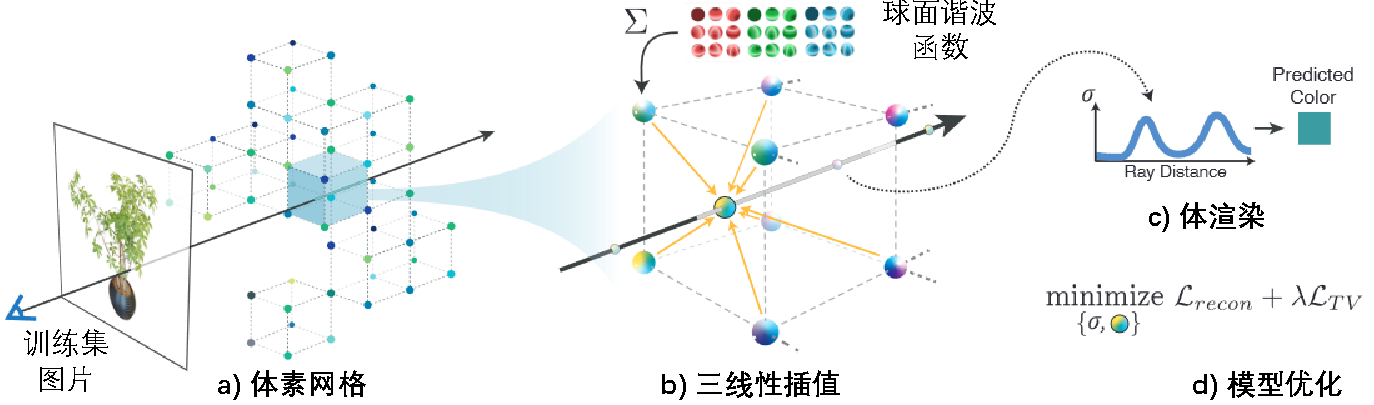
\includegraphics[width=\textwidth]{undergraduate-thesis/images/related-work/plenoxels.pdf}
    \caption{Plenoxels\cite{fridovich-keil_plenoxels_2022} 方法流程图}
    \label{fig:related-work plenoxels pipeline}
\end{figure}

为了弥补这样的缺陷,Plenoxels\cite{fridovich-keil_plenoxels_2022}中提出在三维网格中同时使用球面高斯谐波(Spherical Harmonics, SH)函数来建模场景的视角相关特性,如图\ref{fig:related-work plenoxels pipeline}所示。SH函数可以表示为一组具有不同频率和幅度的球面函数,其中每个函数代表在特定方向上的照射光线所对应的光照贡献。由于球面高斯谐波函数是以角度为参数的球面函数,因此能够很好地表达几何结构与视角之间的关系。通过计算遍历每个像素所对应的差分方程,可以得到具有视角相关效果的图像。从实践上,即是使三维网格在存储场景的辐射颜色和体密度之外,同时存储球面高斯谐波系数组,在查询时通过将插值得到的球面谐波系数带入谐波方程,来计算视角相关颜色。 

\begin{figure}[h]
    \centering
    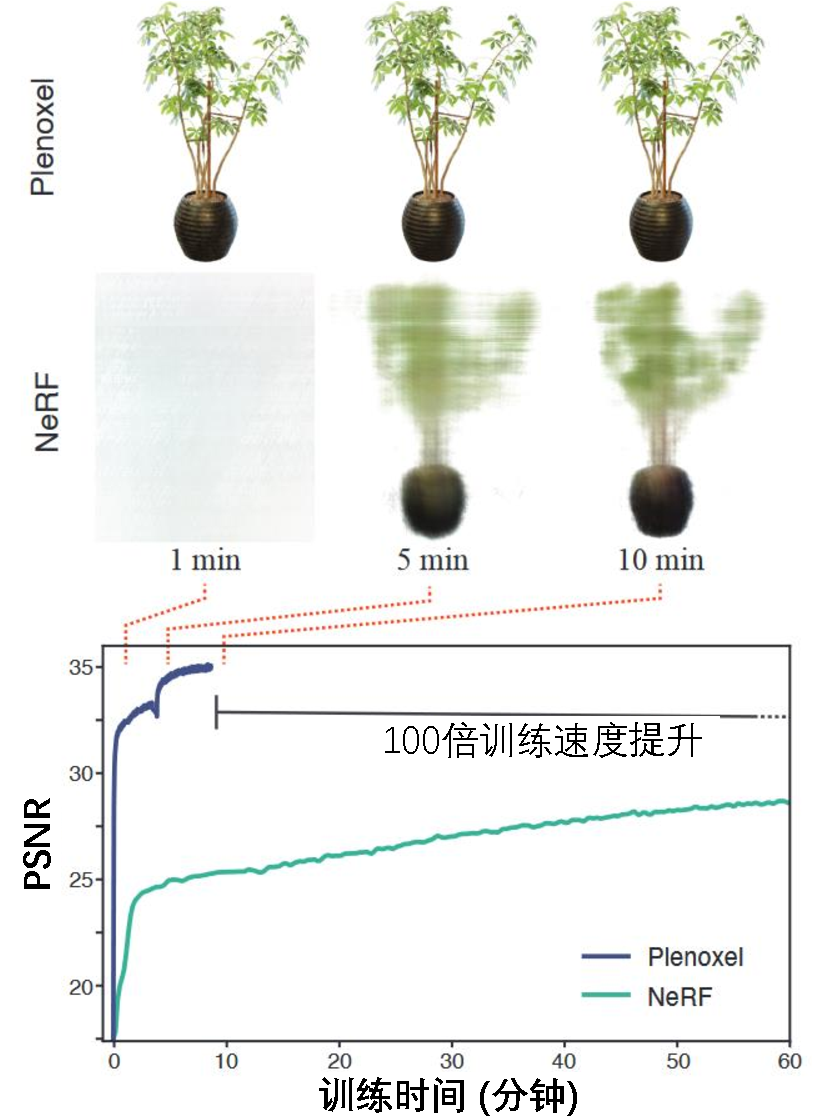
\includegraphics[width=.5\textwidth]{undergraduate-thesis/images/related-work/plenoxels-result.pdf}
    \caption{Plenoxels\cite{fridovich-keil_plenoxels_2022}和原始NeRF\cite{mildenhall_nerf_2020}的性能对比}
    \label{fig:related-work plenoxels-result}
\end{figure}

图\ref{fig:related-work plenoxels-result}中展示了Plenoxels方法和NeRF方法的性能对比,其中横轴为训练时间,纵轴为PSNR指标(越高越好)。由图可知,使用密集体素网格可以为隐式场训练带来成百倍的速度提升,且在最终渲染的效果上也要优于基于多层感知机的方法。

除此以外,当使用密集体素网格重建三维隐式表面时,由于体素网格不能提供多层感知机中的平滑特性(我们将在\ref{sec: related-work density-distance fields}节中讨论该特性),重建的三维表面通常会出现嘈杂的现象(图\ref{fig:related-work monosdf result})。

\subsubsection{隐式体素参数网格地图}
虽然上述的密集体素网格在渲染速度和效果上均有较大的提升,然而在面对更大规模的场景时,仅使用密集网格存储隐函数信息的网络表达能力并不足够,且使用密集网格进行表面重建也会遇到嘈杂的结果,为此,人们提出在网格中存储空间特征而非显式的隐函数值\cite{liu_neural_2021, takikawa_neural_2021, yu_monosdf_2022, huang_di-fusion_2021, peng_convolutional_2020},并使用一个后续的多层感知机解码器来计算最终隐函数值。

记分辨率为$R\times R\times R$的参数网格为$\Phi_\theta$, 多层感知机解码器为$f_\theta$,则使用参数网格来计算隐式函数值可以表示为:
\begin{equation}
    \hat{s} = f_\theta(\gamma(\mathbf{x}), \mathtt{interp}(\mathbf{x}, \Phi_\theta),
\end{equation}
其中$\gamma(\mathbf{x})$为$\mathbf{x}$的位置编码,我们将在\ref{sec: related-work positional encoding}一节讨论位置编码。

在此指上,为了进一步提高网络在场景细节上的建模能力,人们引入了多分辨率的体素参数网格地图\cite{yu_monosdf_2022},即使用多个不同分辨率的网格$\{\Phi^l_\theta\}^L_{l=1}$代替单一参数网格$\Phi_\theta$。记所有不同分辨率的网格中最小的网格($l=1$)的分辨率为$R_{\min}^3$,最大的网格($l=L$)分辨率为$R_{\max}^3$,则第$l$大的网格的分辨率可以表示为:
\begin{equation}
    R_l:=R_{\min}\cdot b^l, \quad l=\mathtt{floor}(\exp(\frac{1}{L - 1}(\ln R_{\max} - \ln R_{\min}))),
\end{equation}
进一步,查询多分辨体素参数网格的过程可以表示为:
\begin{equation}
    \hat{s} = f_\theta(\gamma(\mathbf{x}), \mathtt{concat}\{\mathtt{interp}(\mathbf{x}, \Phi_\theta^l)\}_{l=1}^L),
\end{equation}
$\mathtt{floor}$为下取整函数,$\mathtt{concat}$表示参数拼接。

\begin{figure}[ht]
    \centering
    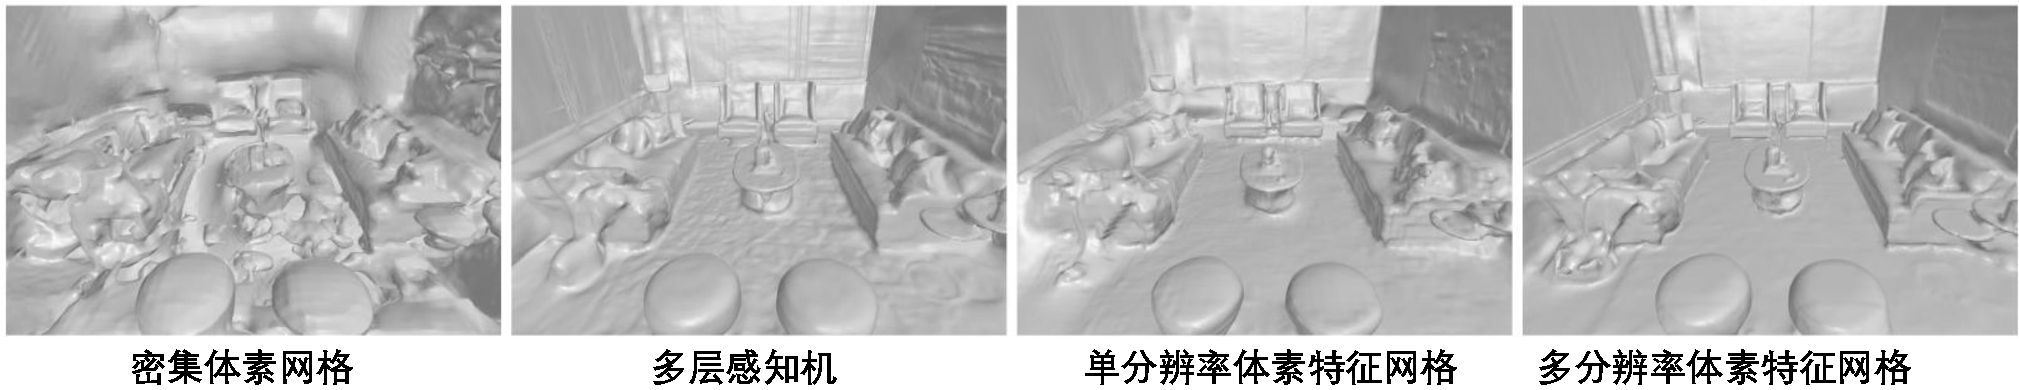
\includegraphics[width=\textwidth]{undergraduate-thesis/images/related-work/monosdf-result.pdf}
    \caption{使用多层感知机、密集体素网格、体素特征网格和多分辨率体素特征网格进行场景SDF学习的结果\cite{yu_monosdf_2022}。}
    \label{fig:related-work monosdf result}
\end{figure}

我们在图\ref{fig:related-work monosdf result}中比较神经隐式表面表示的不同设计选择,我们观察到密集的 SDF 网格会导致嘈杂的重建结果,而 MLP 和单分辨率体素网格改进了结果,但重建的几何图形往往过于平滑而缺少细节,使用多分辨率体素网格可获得较好的结果。

\subsubsection{基于哈希编码的体素参数网格地图}
由于体素参数地图方法在存储大规模场景时,需要使用高分辨率的参数网格来获得足够的细节并保证精度,这导致了空间复杂度高达$\mathcal{O}(N^3)$。然而,在三维场景中,人们通常只关注表面,其所需要的数据量只随场景大小呈平方的空间复杂度($\mathcal{O}(N^2)$)。为了解决这一问题,M\"uller等人提出了一种基于哈希编码的体素参数网格地图——InstantNGP\cite{muller_instant_2022}。 InstantNGP使用哈希表来存储隐式函数值,只需控制哈希表的大小随场景大小平方增长即可。

\begin{figure}[ht]
    \centering
    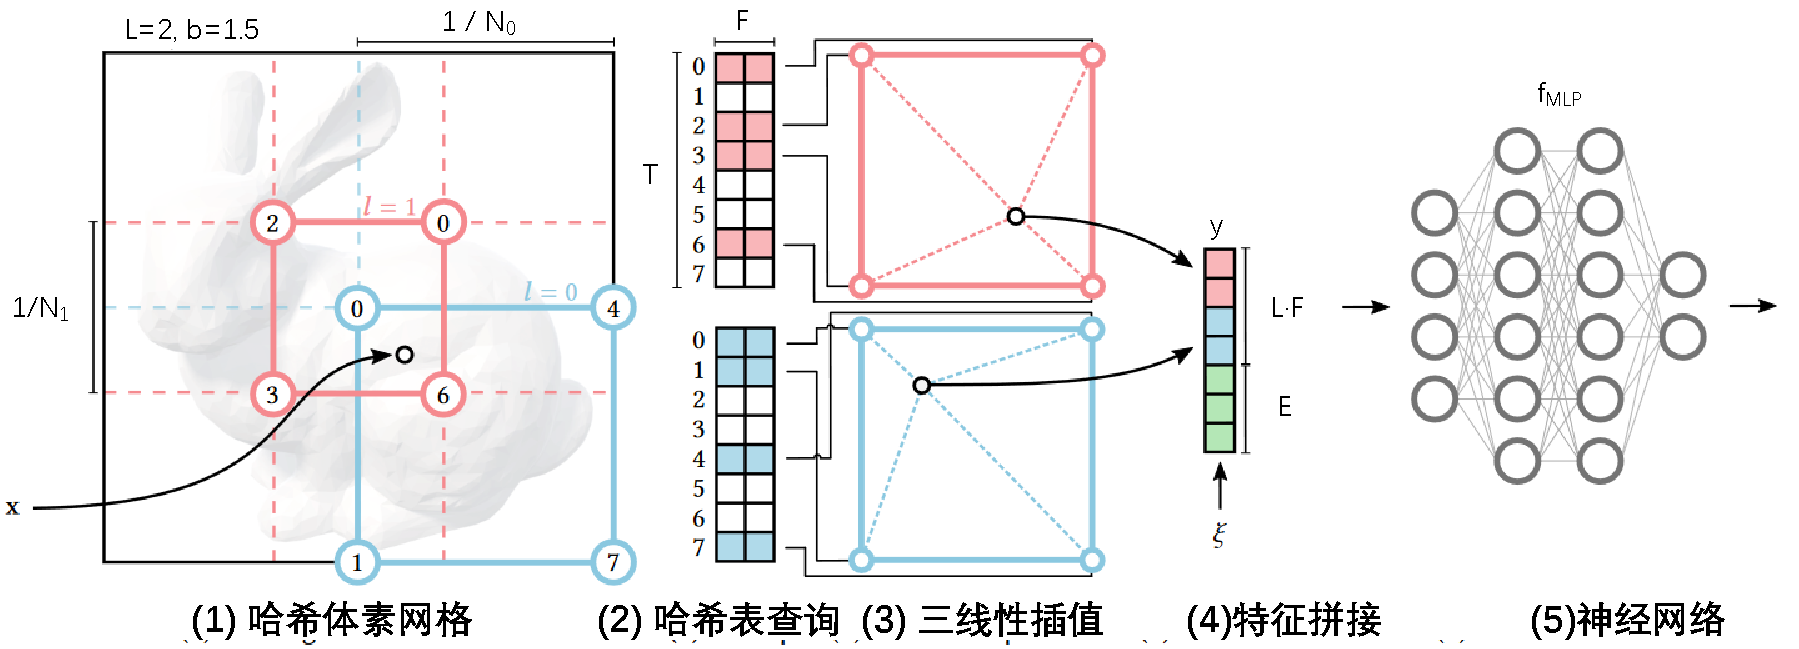
\includegraphics[width=\textwidth]{undergraduate-thesis/images/related-work/instantngp.pdf}
    \caption{InstantNGP\cite{muller_instant_2022} 方法流程图}
    \label{fig:related-work instantngp}
\end{figure}

如图\ref{fig:related-work instantngp}所示,InstantNGP沿用了多分辨率体素网格的基本框架,在查询任意一点的三维场景隐函数值时,首先需要查询其在各个层次的网格上的八个相邻节点,接着将节点编号作为索引查询哈希表,将查询结果经三线性插值之后拼接形成三维点特征。我们可以将这个过程表示为:
\begin{equation}
    \hat{s} = f_\theta(\gamma(\mathbf{x}), \mathtt{concat}\{\mathtt{interp}(h^l(\mathbf{x}), \Phi_\theta)\}_{l=1}^L),
\end{equation}
其中$h^l(\mathbf{x})$为哈希函数,在InstantNGP中,每个级别的参数网格使用不同的哈希函数:
\begin{equation}
    h^l(\mathbf{x}) = \left(\bigoplus_{i}x_i\pi_i^l\right) \text{mod} T,
\end{equation}
$T, \pi^l$为随机大质数。

\subsection{低维张量地图表示}
\label{sec: related-work multi-plane-based implicit representations}
\subsubsection{基于张量分解的向量-矩阵地图表示}
虽然InstantNGP基于哈希表的存储数据结构可以有效地缓解基于体素网格的场景表示中高空间复杂性的问题,然而研究者发现现有方法所使用的体素网格中绝大部分体素均属于空白空间,因而网格的使用率实际并不高。Anpei等人\cite{chen_tensorf_2022}的工作TensoRF中利用了一个事实,即特征网格可以自然地被视为 4D 张量,其中它的三个模式对应于网格的 XYZ 轴,第四个模式代表特征通道维度,从而解决了体素网格表示的低效问题,从而产生了一系列简单而有效的方法。TensoRF利用经典张量分解技术(已广泛应用于各个领域的高维数据分析和压缩 \cite{kolda_tensor_2009}),将辐射场的张量分解为多个低秩张量分量,从而获得准确且紧凑的场景表示。

\begin{figure}[h]
    \centering
    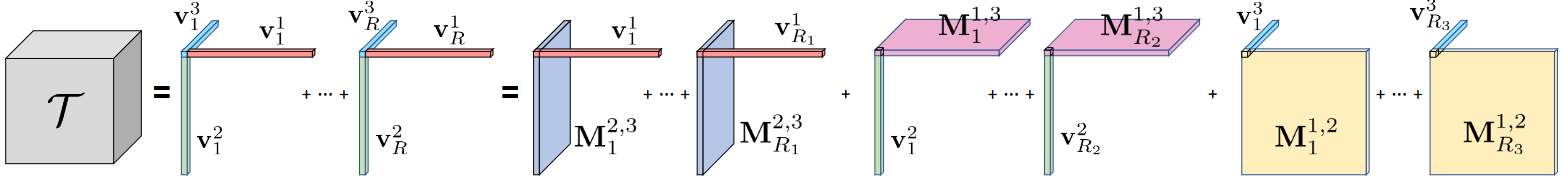
\includegraphics[width=\textwidth]{undergraduate-thesis/images/related-work/Tensor Decomp.png}
    \caption{张量分解\cite{chen_tensorf_2022}。左图:CP 分解,它将张量分解为向量外积之和。右图:TensoRF的向量矩阵分解,它将张量分解为向量矩阵外积的总和。}
    \label{fig:related-work tensor-decomp}
\end{figure}

传统的CP张量分解(如式\ref{eq: related-work CP decomp}所示),将三维张量$\mathcal{T}\in\mathbb{R}^{I\times J\times K}$分解为三组秩为一的向量乘积的和。TensoRF将CP分解拓展为向量-矩阵分解模式(如式\ref{eq: related-work TensoRF decomp}所示)。对于每个分解单元,我们将CP-分解中的其中两个分量合并,不使用单独的向量,而是组合每两个模式并用矩阵表示它们,从而允许每个分解单元使用较少数量的组件进行充分参数化。
\begin{equation}
    \mathcal{T} = \sum_{r=1}^R\mathbf{v}_r^1\circ\mathbf{v}_r^2\circ\mathbf{v}_r^3
    \label{eq: related-work CP decomp}
\end{equation}

\begin{equation}
    \mathcal{T} = \sum_{r=1}^R\mathbf{v}_r^X\circ\mathbf{M}_r^{Y,Z}+\mathbf{v}_r^Y\circ\mathbf{M}_r^{X,Z}+\mathbf{v}_r^Z\circ\mathbf{M}_r^{X,Y}
    \label{eq: related-work TensoRF decomp}
\end{equation}

TensorRF (VM)使用一组向量 ($\mathbf{v}$) 和矩阵 ($\mathbf{M}$) 将辐射场建模为张量,它们沿相应的 (XYZ) 轴描述场景,并用于计算可微分光线行进中的体积密度 $\sigma$ 和视角相关颜色 $c$。对于每个着色位置$ \mathbf{x} = (x, y, z)$,我们使用来自向量/矩阵因子的线性/双线性插值结果来有效地计算张量分量的特征。该特征被进一步用于渲染,从而得到一个紧致的神经隐式表示。

\begin{figure}[ht]
    \centering
    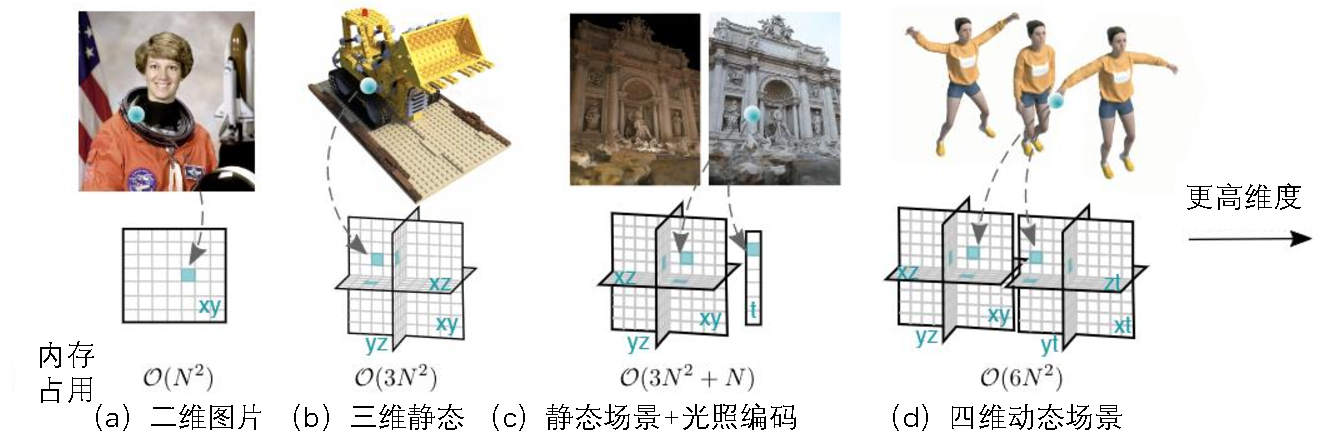
\includegraphics[width=\textwidth]{undergraduate-thesis/images/related-work/kplanes-teaser.pdf}
    \caption{$d$ 维空间的平面分解示意图\cite{fridovich-keil_k-planes_2023}。}
    \label{fig:related-work kplane-teaser}
\end{figure}

\subsubsection{多平面地图表示}
受TensoRF启发,研究者进一步将张量分解的概念进一步泛化,仅使用多个互相正交的平面来代替体素网格\cite{fridovich-keil_k-planes_2023, cao_hexplane_2023, reiser_merf_2023, chan_efficient_2022}。其中K-Planes\cite{fridovich-keil_k-planes_2023}将$d$维体素张量使用$k=\frac{d(d-1)}{2}$个平面表示,即$d$个维度的任意两维均用一个平面表示,如图\ref{fig:related-work kplane-teaser}所示。例如,对于静态 3D 场景,这会产生三平面,其中3个平面代表 XY、XZ 和 YZ。而对于动态 4D 场景,这会产生六平面,其中6 个平面,包括三个纯空间平面和三个时空平面 X-t、Y-t 和 Z-t。如果我们希望表示一个 5D 空间,我们可以使用$\frac{5\times4}{2}=10$个平面。


\begin{figure}[h]
    \centering
    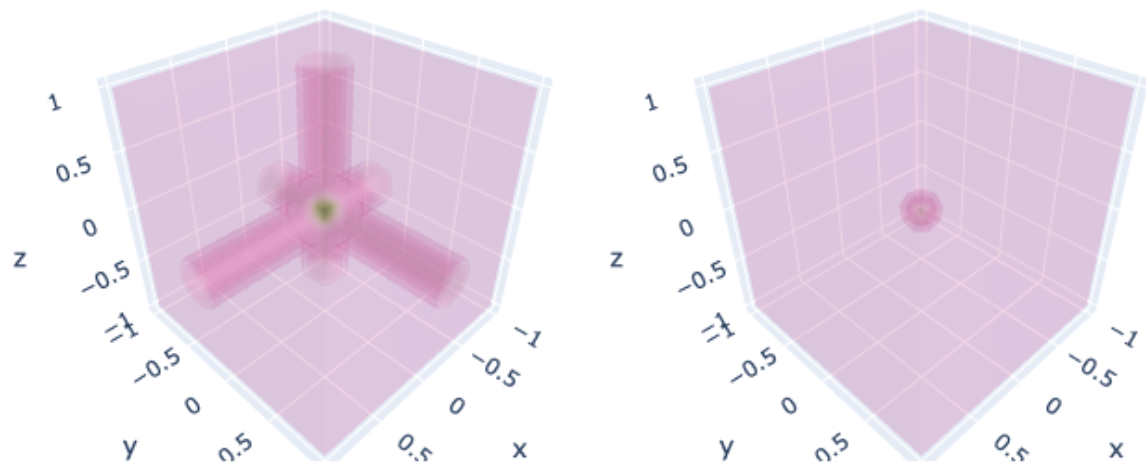
\includegraphics[width=\textwidth]{undergraduate-thesis/images/related-work/hadamard-product.png}
    \caption{平面特征的逐元素加法(左)与乘法(右)的比较。在这两种情况下,假设每个平面中只有单个条目为+1,其余部分均为零,通过乘法可以选择单个 3D 点,但通过加法只能产生相交线。这说明乘法可以提高显式模型的表达能力\cite{fridovich-keil_k-planes_2023}。}
    \label{fig:related-work hadamard-product}
\end{figure}

不同于最早的三平面场景表示\cite{chan_efficient_2022}中使用逐像素的求和来整合各平面上的特征,K-Planes中使用Hadamard乘积来获取空域感知的特征信号(如\ref{fig:related-work hadamard-product}所示),即:
\begin{equation}
    f(\mathbf{q}) = \prod_{c\in C}f(\mathbf{q})_c,
\end{equation}
其中$c\in C$为场景中的平面集合,在每个平面中查询$\mathbf{q}$点处的特征,通过逐像素求乘积得到高维空间中点的特征。

\subsection{小结}
在本节中,我们介绍了神经隐式场出现以来,所使用的场景表示从多层感知机\cite{mildenhall_nerf_2020,park_deepsdf_2019, mescheder_occupancy_2019, shim_snerl_2023, zhi_-place_2021}逐渐发展为体素网格\cite{fridovich-keil_plenoxels_2022,yu_monosdf_2022,muller_instant_2022,jiang_instantavatar_2022}、多平面\cite{chen_tensorf_2022,fridovich-keil_k-planes_2023,cao_hexplane_2023}等场景表示方法。

虽然多平面的方法可以对一个简单场景进行高效、准确的表示学习,但我们发现,当场景规模逐渐从物体、室内场景基本扩展到室外自动驾驶大场景下时,使用单一的多平面场景表示反而会产生退化的效果。在本文中,我们将提出一种混合场景表示方法,使得即便在更大规模的复杂场景中,依然可以用较小的存储空间获得准确的场景表示。

\newpage
\section{真实感的神经渲染方法:场景扭曲变换}
\label{sec: related-work realistic rendering}
除了使用不同的场景表示方法外,为了实现更真实的渲染效果,研究者还在其他方面做出了改进。其中,最为典型的方法是将三维欧式空间通过变换,映射到扭曲后的参数空间。

通常来讲,在场景图片数据集中,场景的内容在三维空间上并不是均匀分布的,如在前向观察的数据集中,通常场景内容随着深度的增加而反比例下降;在无边界、物体中心的数据集中,场景内容随着空间点到物体中心距离的增加而下降。因此,若能将在原始三维欧式空间中非均匀分布的空间点映射到一个均匀分布,则将能大大提升场景表示的利用率,从而提高渲染真实感。

\subsection{位置编码}
\label{sec: related-work positional encoding}

尽管神经网络被证明为通用的函数逼近器\cite{hornik_multilayer_1989},但研究者发现让网络直接在 输入坐标$(x,y,z,\theta,\phi)$上优化会导致渲染颜色。机器学习领域相关工作\cite{rahaman_spectral_2019}表明多层感知机偏向于学习低频函数,在高频信息上的学习速率显著低于低频信息的学习速率。而在将输入传递到网络之前,使用高频函数将输入映射到更高维空间可以更好地拟合包含高频变化的数据。

位置编码是一种常用于自注意力机制的技术,它通过将空间位置信息编码为向量来提高神经网络的表现力。但是Transformers\cite{vaswani_attention_2017}等基于注意力机制的方法为Token在整个序列中的离散位置提供隐式的位置坐标,然而在NeRF\cite{mildenhall_nerf_2020}中,通过将场景中的位置信息编码为含有位置信息的高维向量,可以将输入的xyz坐标映射到高维空间中,从而让网络学习场景中的高频细节信息,实现更真实的渲染效果。NeRF位置编码将输入数据$p$通过式\ref{eq: related-work PE}所示的方法映射到高维频域空间。
\begin{equation}
    \gamma(p) = \left(\sin(2^0\pi p),\cos(2^0\pi p),\cdots \sin(2^{L-1}\pi p),\cos(2^{L-1}\pi p)\right)
    \label{eq: related-work PE}
\end{equation}

\begin{figure}[ht]
    \centering
    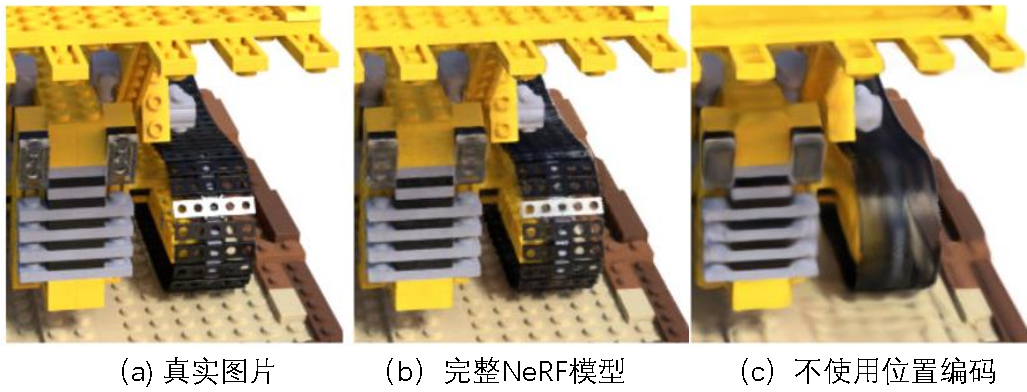
\includegraphics[width=\textwidth]{undergraduate-thesis/images/related-work/NeRF ablation-PE.pdf}
    \caption{位置编码对NeRF网络性能的影响\cite{mildenhall_nerf_2020}。}
    \label{fig:related-work nerf-PE-ablation}
\end{figure}

图\ref{fig:related-work nerf-PE-ablation}中展示了去掉位置编码后对NeRF网络渲染图片的效果影响。由图可以看出,去除高频位置信息后,NeRF网络很难表示图片中的高维几何细节,从而表现出“模糊”的特点。

从本质上,NeRF的位置编码实质上也是一个扭曲变换,将信息分布不均匀的空域映射到更加均匀的频域空间。

\subsection{基于Mip的反走样神经渲染}
尽管神经辐射场\cite{mildenhall_nerf_2020}及其变体\cite{muller_instant_2022,martin-brualla_nerf_2021,zhang_nerf_2020}在视图合成任务中展示了令人印象深刻的结果,但 NeRF 的渲染模型存在缺陷:当训练图像以多种分辨率观察场景内容,或分别从远处和近处观察同一位置时,NeRF的渲染在近景视图中显得过于模糊,并且在远景视图中包含混叠伪影。其原因在于NeRF将一个像素抽象为一个无穷小的没有面积的三维点,然而在真实世界中,像素在空间上占有一定的面积,从而相机发出的“光线”实际上应该表示为一个圆锥体(如图\ref{fig:related-work mip-nerf cone tracing}所示)。式\ref{eq: related-work volume rendering}中的NeRF渲染公式仅在一条射线上积分所有的辐射值,使用线积分的结果代替了视锥中全部三维点的重积分:
\begin{equation}
    c = \iiint_{\mathbf{p}\in V}\sigma(\mathbf{p})T(\mathbf{p})c(\mathbf{p},\mathbf{d})\text{d}p,
\end{equation}
其中$V$为相机原点$\mathbf{o}$朝方向$\mathbf{d}$发射的视锥,$p$为$V$中点。

\begin{figure}[h]
    \centering
    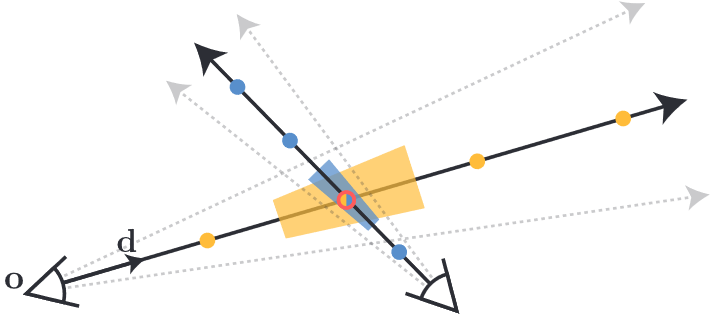
\includegraphics[width=0.8\textwidth]{undergraduate-thesis/images/related-work/mipnerf-intersection.png}
    \caption{NeRF方法产生走样原因的示意图\cite{barron_mip-nerf_2021}。}
    \label{fig:related-work mip-nerf intersection}
\end{figure}

这样的简化必然会导致渲染误差的存在,进而产生走样的渲染结果。如图\ref{fig:related-work mip-nerf intersection}所示,当我们分别从两个不同远近、不同角度的视角同时观察到空间中的某个三维点。NeRF沿着每个像素的光线提取点采样位置编码特征,这些点采样特征忽略了每条射线观察到的体积的形状和大小,因此两个不同的相机以不同的比例对同一位置进行成像可能会产生相同的模糊点采样特征,从而显着降低 NeRF 的性能。

\begin{figure}[h]
    \centering
    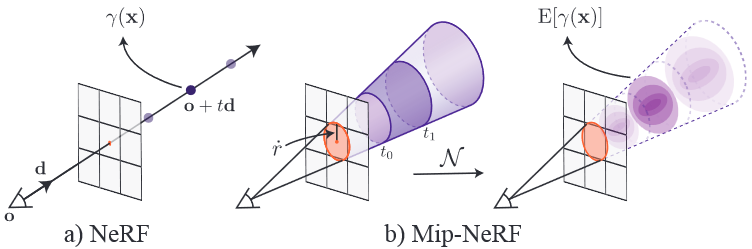
\includegraphics[width=\textwidth]{undergraduate-thesis/images/related-work/mipnerf-cone.png}
    \caption{NeRF (a) 沿着从相机投影中心通过每个像素的光线进行采样,然后使用位置编码 (PE) $\gamma$ 对这些点进行编码以产生特征$\gamma(x)$。 Mip-NeRF (b) 对由相机像素定义的 3D 圆锥台进行推理,使用集成位置编码 (IPE) 对这些锥形截锥体进行特征化,使用多元高斯近似截锥体,然后计算积分 $E[\gamma(x)]$以近似超采样的效果\cite{barron_mip-nerf_2021}。}
    \label{fig:related-work mip-nerf cone tracing}
\end{figure}

一个直接的解决方案是采用离线光线追踪中使用的策略:通过发射多条光线并对每个像素进行超采样。但这对于像 NeRF 这样的神经体积表示来说是非常昂贵的,它需要数百次查询多层感知机网络来渲染一条射线,并需要几个小时甚至几天来重建一个场景。Mip-NeRF \cite{barron_mip-nerf_2021}提出将采样过程显式建模为投射锥体而不是射线的过程,并对每个采样的锥台使用一个各向异性的高斯椭球表示。为了模拟对整个锥台进行超采样,Mip-NeRF提出用高斯椭球上位置编码的均值近似每个锥台内体积的位置编码的平均,即集成位置编码(Integrated Positional Encoding,IPE)。
\begin{figure}[h]
    \centering
    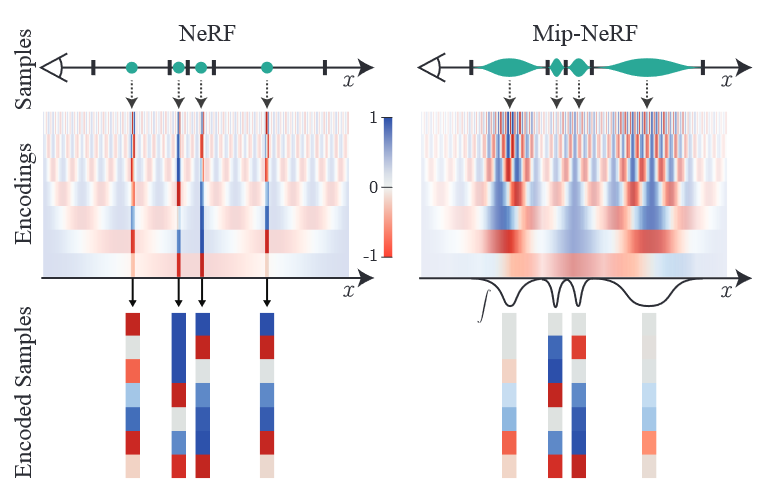
\includegraphics[width=\textwidth]{undergraduate-thesis/images/related-work/mipnerf-encoding.png}
    \caption{NeRF(左)和集成位置编码(IPE)(右)的一维可视化。由于 NeRF 沿每条射线对点进行采样并对所有频率进行同等编码,因此高频 PE 特征混叠,从而导致渲染伪影。通过在每个区间上使用集成位置编码特征,当频率周期与被集成的间隔大小相近时,IPE特征的高频维度缩小到零,从而产生隐式编码大小的抗锯齿特征。\cite{barron_mip-nerf_2021}}
    \label{fig:related-work mip-nerf encoding}
\end{figure}

具体来讲,高斯椭球$(\mu,\Sigma)$内的集成位置编码可以写作:
\begin{align}
    \gamma(\mu,\Sigma) &= \text{E}_{\mathbf{x}\sim\mathcal{N}(\mu_\gamma,\Sigma_\gamma)}[\gamma(\mathbf{x})] \\
    &= \begin{bmatrix}
    \sin(\mu_\gamma)\circ\exp(-\frac{1}{2}\text{diag}(\Sigma_\gamma))\\
    \cos(\mu_\gamma)\circ\exp(-\frac{1}{2}\text{diag}(\Sigma_\gamma))
    \end{bmatrix}
\end{align}

由图\ref{fig:related-work mip-nerf encoding},IPE 特征的行为很直观:如果位置编码中的特定频率的周期大于用于构造 IPE 特征的区间宽度,则该频率的编码不受影响。但是,如果周期小于间隔,则该频率的编码将按比例缩小至零。简而言之,IPE 保留了在一个区间内恒定的频率并温和地“移除”在一个区间内变化的频率,而 PE 保留了直到某个手动调整的超参数 L的所有频率。通过以这种方式缩放每个三角函数值,IPE可以有效地抗锯齿位置编码功能,可以平滑地编码空间体积的大小和形状。

\begin{figure}[h]
    \centering
    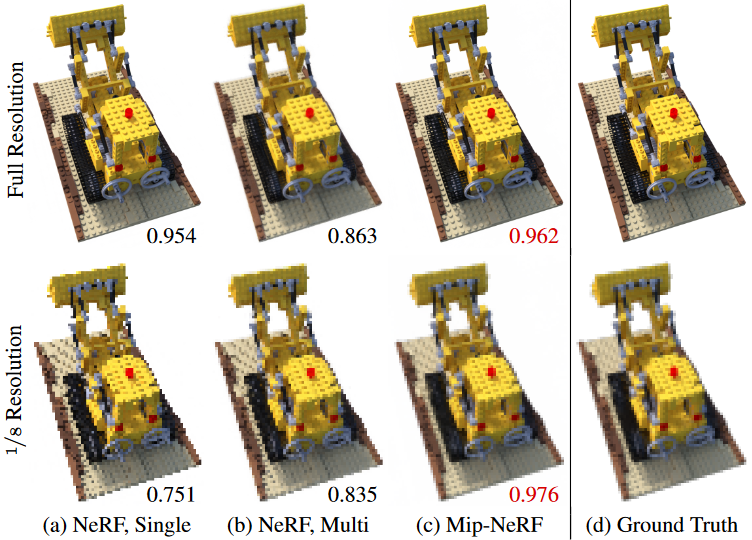
\includegraphics[width=0.8\textwidth]{undergraduate-thesis/images/related-work/mipnerf-multi-scale.png}
    \caption{Mip-NeRF\cite{barron_mip-nerf_2021} 和基线模型在不同图片分辨率上渲染的效果对比。}
    \label{fig:related-work mip-nerf results}
\end{figure}

图\ref{fig:related-work mip-nerf results}展示了Mip-NeRF使用IPE后与其他模型在渲染低分辨率图像时的效果对比。在全分辨率图像上训练的 NeRF 能够在新的视图位置生成逼真的渲染图,但仅限于训练图像的分辨率或比例;将相机向后拉并放大(或类似地,调整相机内在特性以降低图像分辨率)会导致呈现出严重的锯齿现象;在多分辨率图像上训练 NeRF 可以稍微改善这个问题,但会导致跨尺度渲染质量差:全分辨率模糊,低分辨率出现“锯齿”; Mip-NeRF也在多分辨率图像上训练,但能够在不同尺度上生成逼真的渲染。

\subsection{无界场景表示}
相比原始的位置编码和Mip-NeRF中的集成位置编码,Mip-NeRF中的无界场景映射则是一种更加直观的扭曲映射方法。

由于透视投影,远离相机放置的物体将占据图像平面的一小部分,但如果放置在附近,则会占据更多图像并且细节可见。因此,理想的 3D 场景参数化应该为附近的内容分配更多的容量,为远处的内容分配更少的容量。

最初的 NeRF 论文侧重于从360$^\circ$捕获具有蒙版背景的对象以及所有图像面向大致相同方向的正面场景(也称作Forward-Facing)。对于蒙面物体,NeRF 直接参数化 3D 欧几里得空间中的场景,但对于正面场景,NeRF 使用投影空间中定义的坐标(归一化设备坐标,或“NDC”空间)。通过将无限深的相机视锥变形为有界立方体,其中沿 z 轴的距离对应于视差(反距离),NDC 以与透视投影的几何形状一致的方式有效地重新分配 NeRF MLP 的容量。然而,在所有方向上都是无界的场景,而不仅仅是在一个方向上,需要不同的参数化。 不同于NeRF++\cite{zhang_nerf_2020}使用额外的网络对远处的物体进行建模,在Mip-NeRF 360\cite{barron_mip-nerf_2022}中,将这个想法扩展到 Mip-NeRF 并提出了一种将任何平滑参数化应用于体积的无界场景参数化方法。

\begin{figure}[ht]
    \centering
    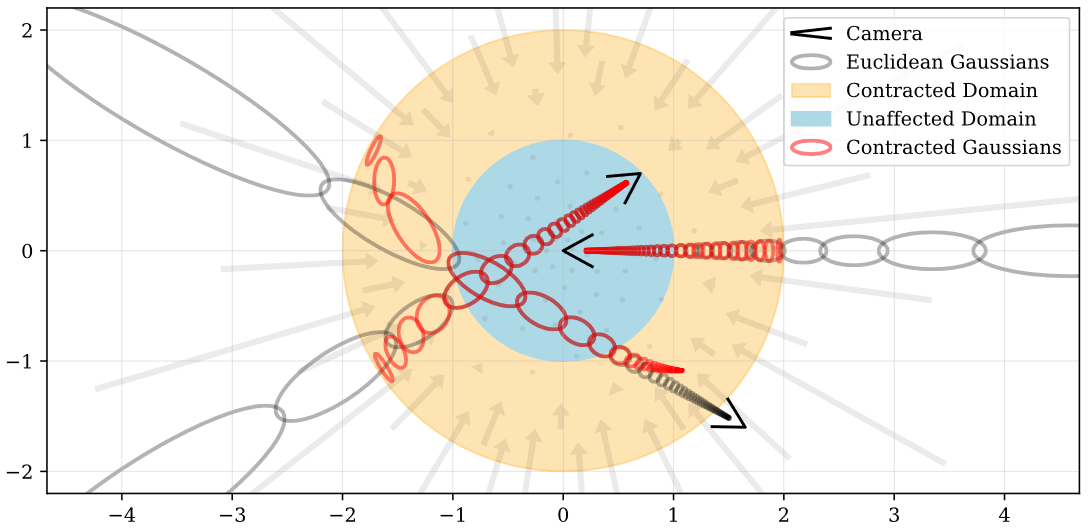
\includegraphics[width=\textwidth]{undergraduate-thesis/images/mipnerf360-contraction.png}
    \caption{Mip-NeRF 360\cite{barron_mip-nerf_2022}的无界场景压缩的二维示意图}
    \label{fig:related-work-unbounded-contraction}
\end{figure}

如图\ref{fig:related-work-unbounded-contraction}所示,对于任意一个输入坐标$x\in\mathbb{R}^3$,Mip-NeRF 360将输入坐标通过下面的公式映射到一个半径为2的球面内:
\begin{equation}
    \mathtt{contract}(\mathbf{x}) = \left\{\begin{matrix}&\mathbf{x}&||\mathbf{x}||<1\\&(2-\frac{1}{||\mathbf{x}||})(\frac{\mathbf{x}}{||\mathbf{x}||})&||\mathbf{x}||\geq1\end{matrix}\right.
\end{equation}

\subsection{小结}
在本节中,我们介绍了使用场景扭曲变换提高场景表示模型利用率的几种方法,然而目前的扭曲变换方法无法解决在更大规模的室内、室外复杂场景的高效表达,因而限制了神经隐式场在自动驾驶等领域的发展。在本文中我们提出基于神经点云的场景扭曲变换,使得场景表示可以自适应地拟合大规模场景。


\newpage
\section{辐射-距离混合隐式场}
\label{sec: related-work density-distance fields}
在本章的前两节中,我们介绍了以神经辐射场的神经场景表示的发展,然而单一的辐射场景表示对于场景几何的建模能力较差。在本节中,我们将首先分析辐射场这一不足的原因,接着分别从采样策略、体渲染模型、多元传感信息融合和混合隐式场优化的几个方面介绍辐射-距离混合隐式场。

\subsection{神经辐射场的形状-辐射二义性}
\label{sec: related-work shape-radiance ambiguity}
在没有正则化的情况下,NeRF\cite{mildenhall_nerf_2020}对仅依赖于视图的外观进行建模的能力导致 3D 形状和辐射之间存在一个二义性,使得网络可以接受退化的内在形状,而渲染出真实感颜色。对于任意的、不正确的形状,可以证明存在一组辐射场可以完美地解释训练图像,但不能很好地推广到新的测试视图。

为了说明这种歧义,假设对于给定的场景,我们将几何体表示为一个单位球体。换句话说,让我们将 NeRF 的不透明度场固定为在单位球体表面为 1,在其他地方为 0。然后,对于每个训练图像中的每个像素,我们将穿过该像素的光线与球体相交,并将交点处(以及沿光线方向)的辐射值定义为该像素的颜色。这个人工构造的解决方案是一个有效的 NeRF 重建,它完美地适合输入图像。

\begin{figure}[h]
    \centering
    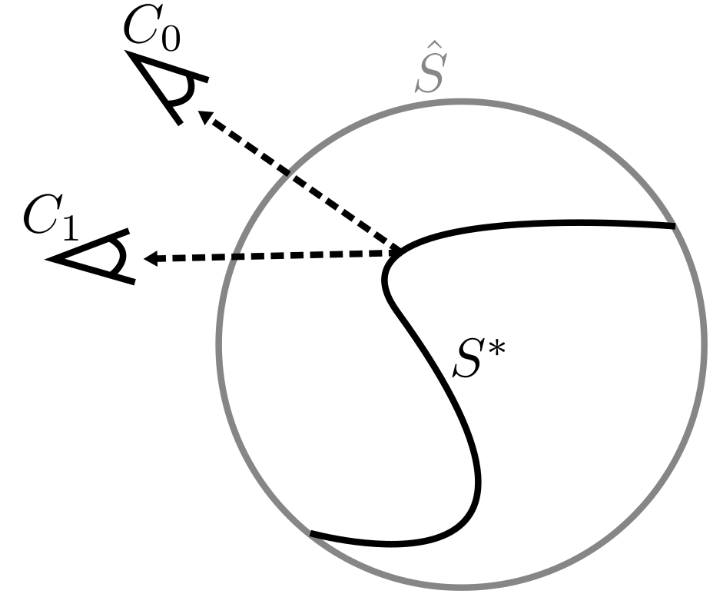
\includegraphics[width=0.6\textwidth]{undergraduate-thesis/images/shape-radiance ambiguity.png}
    \caption{形状-辐射二义性示意图\cite{zhang_nerf_2020}}
    \label{fig:related-work shape-radiance ambiguity}
\end{figure}

如图\ref{fig:related-work shape-radiance ambiguity}所示,假设一个二维曲面$S^*$的形状为图中所示,相机$C_0, C_1$分别从不同角度观察曲面上一点,由图可以看出,如果网络实际学到的几何形状为图中$\hat{S}$所代表的单位圆,而将$C_0, C_1$观察到的颜色“贴”在单位圆上。这样即使网络学习到的几何与真实几何形状完全不同,也可以渲染出真实感的颜色。这种二义性被叫做“形状-辐射二义性”\cite{zhang_nerf_2020},因而由辐射场建模的场景几何通常被认为是欠约束的。

基于这一观察,近年来,研究者提出同时优化辐射和距离场,并在体渲染过程中将这两个完全不同的隐式场的输出进行融合\cite{oechsle_unisurf_2021,gropp_implicit_2020,yariv_multiview_2020,yariv_volume_2021,wang_neus_2021,shao_doublefield_2022,darmon_improving_2022,ueda_neural_2022,long_sparseneus_2022,yu_monosdf_2022,wang_pet-neus_2023,yuan_monocular_2023,liang_hr-neus_2023,chen_dehazenerf_2023,zhu_vdn-nerf_2023,azinovic_neural_2022, sun_neural_2022}。 简单来说,就是将神经符号距离场(Neural SDF)通过几何变换转换为辐射场中体密度的过程。然而,由于这两种隐式场天然的差距,这一融合并不是一件易事。为了弥补隐式场直接的领域差距,研究者在采样策略\cite{yariv_volume_2021, mildenhall_nerf_2020, barron_mip-nerf_2022, oechsle_unisurf_2021},体渲染方法\cite{oechsle_unisurf_2021,yariv_volume_2021,wang_neus_2021},融合多元传感信息\cite{azinovic_neural_2022,yu_monosdf_2022}和隐式场优化进行了大量的研究工作,如图\ref{fig:related-work sdfstudio}所示\cite{yu_sdfstudio_2022}。

\begin{figure}[t]
    \centering
    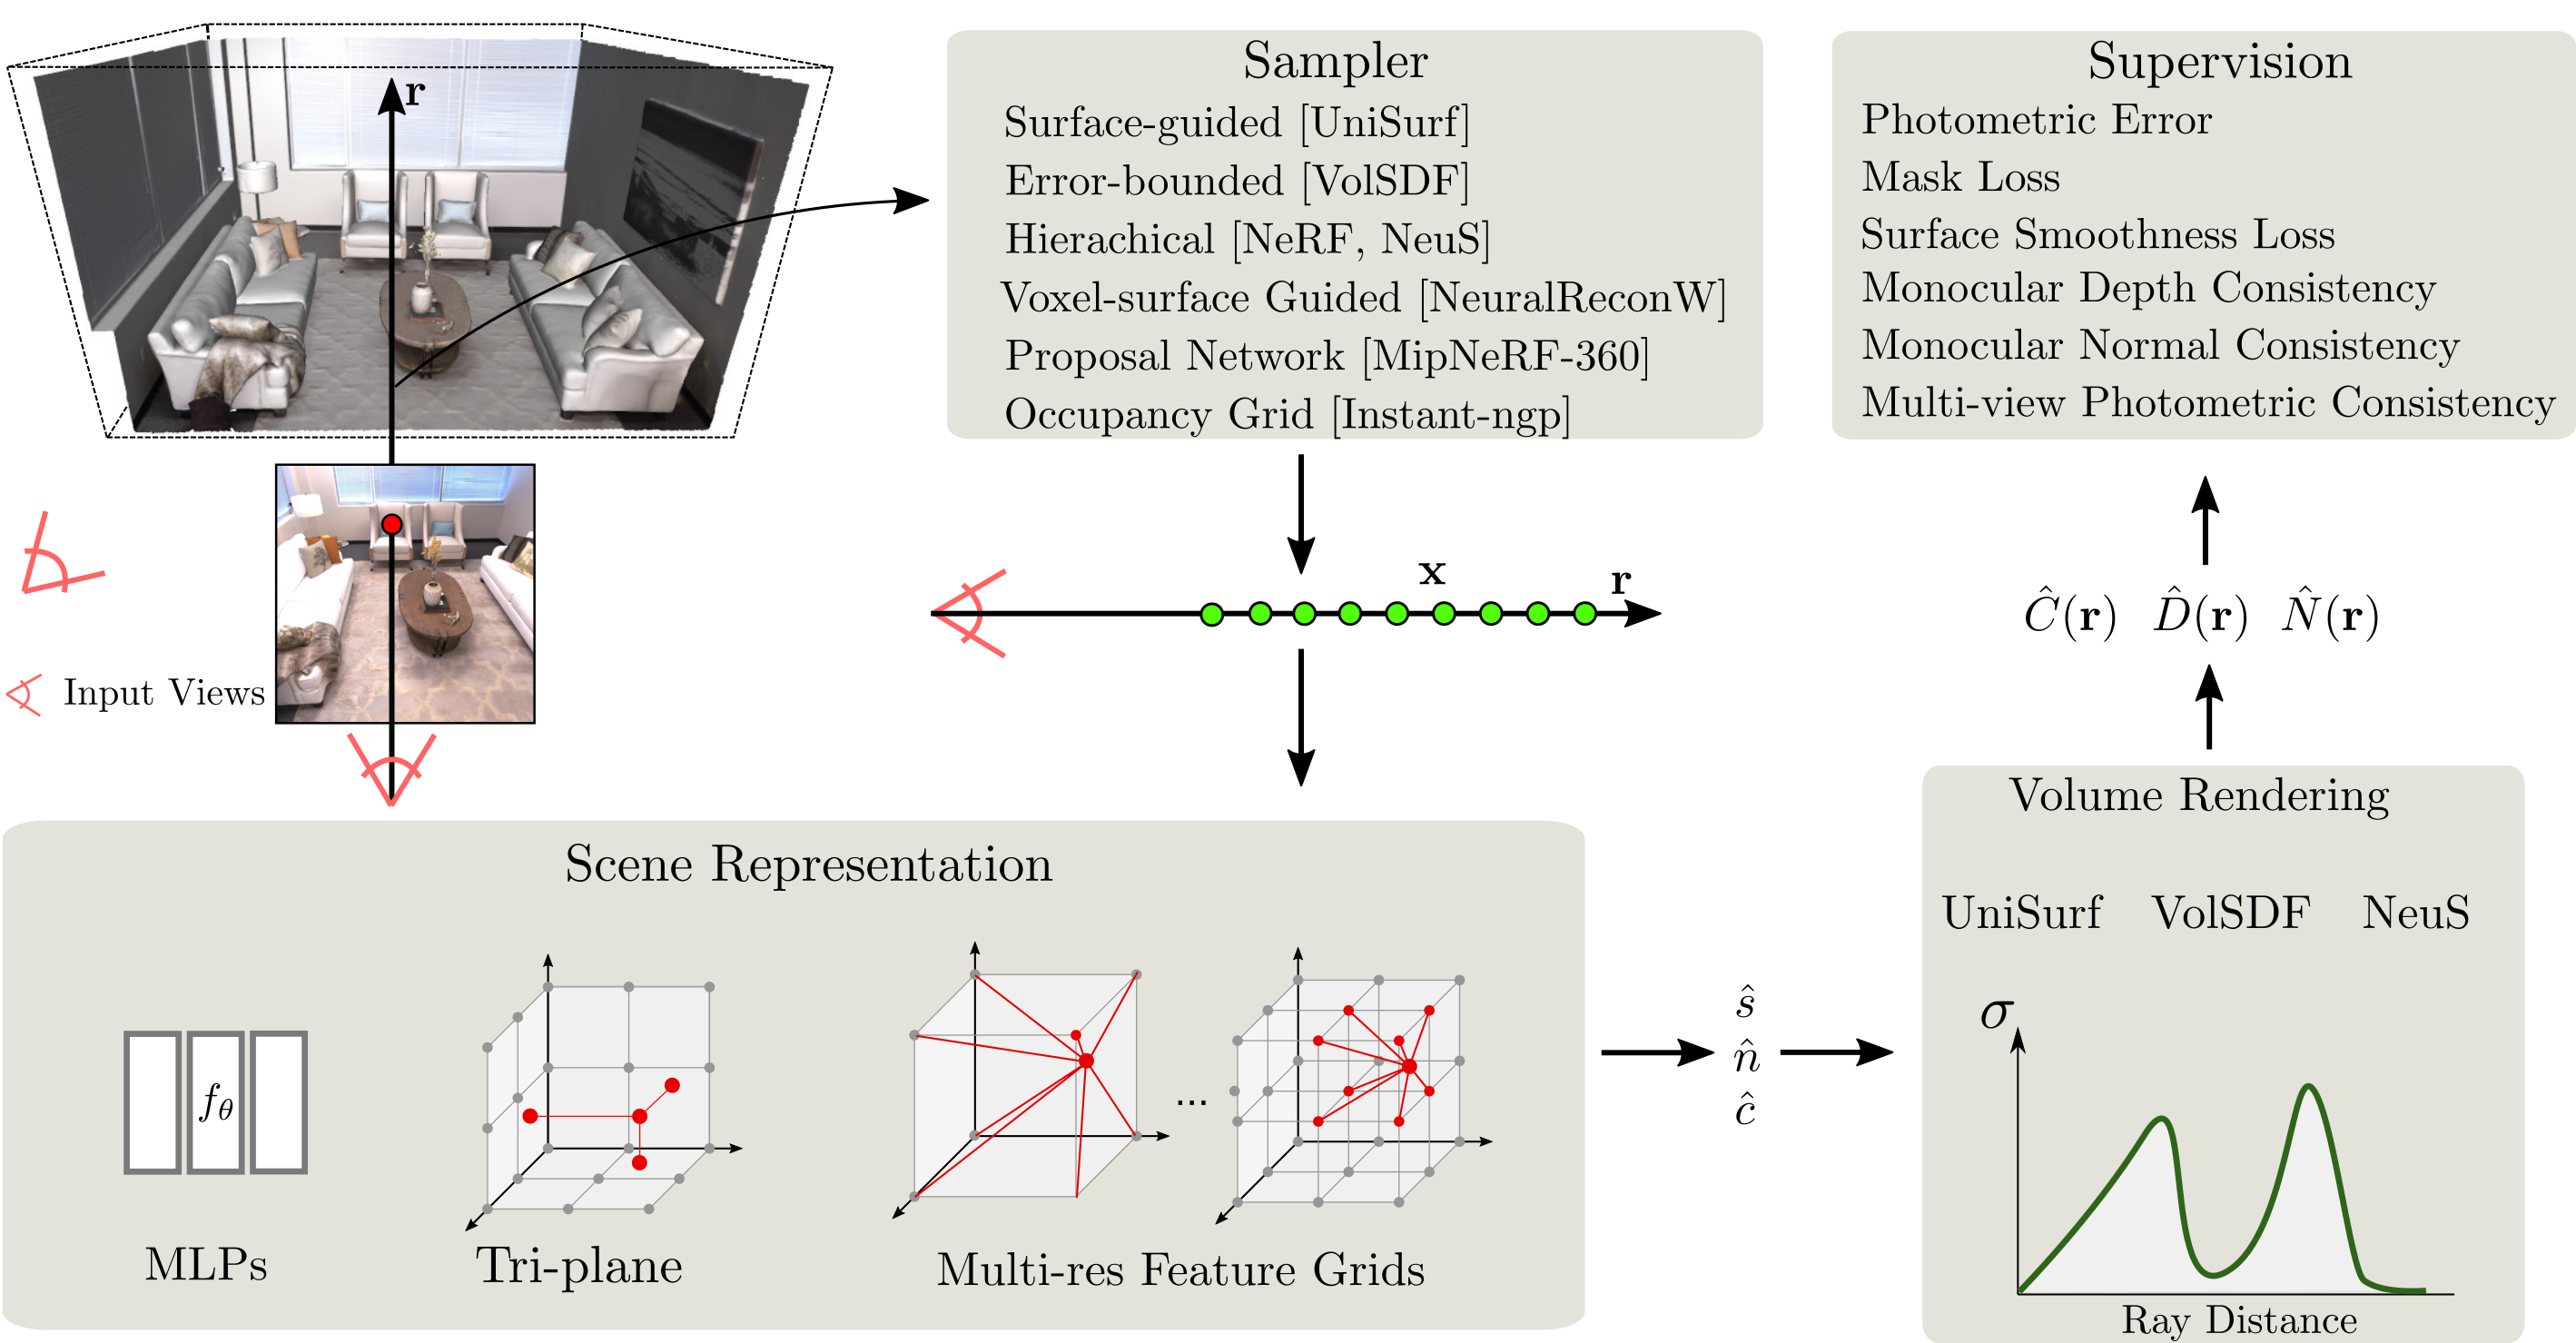
\includegraphics[width=\textwidth]{undergraduate-thesis/images/sdfstudio.png}
    \caption{混合隐式场中各个组件的相关研究工作\cite{yu_sdfstudio_2022}}
    \label{fig:related-work sdfstudio}
\end{figure}

\subsection{采样策略}
神经辐射场中首次将隐式表达用于体积渲染积分的管线中,然而在计算机实现中我们必须对体积积分进行离散化,使用有限的采样点最大限度地还原连续体积中的密度分布。因此,选取合适数量、位置的采样点对于隐式场场景表示学习格外重要。在本节中,我们首先介绍NeRF\cite{mildenhall_nerf_2020}中的分层采样方法,接着介绍后续工作中对该方法的改进。

\subsubsection{分层采样}
\label{sec: coarse-to-fine sampling}
在原始NeRF中,为了估计体渲染积分(公式\ref{eq: related-work volume rendering}),使用了由粗到精的分层采样策略:首先将$[t_n,t_f]$划分为N个均匀分布的区间,然后从每个区间内随机均匀地抽取一个样本(如式\ref{eq: related-work coarse-sampling}),将这些样本通过粗网络后根据体密度分布进行重要性重采样得到精细样本,最后将两次抽取的采样点通过精细网络进行渲染。
\begin{equation}
    t_i\sim\mathcal{U}\left[t_n+\frac{i-1}{N}(t_f-t_n), t_n+\frac{i}{N}(t_f-t_n)\right]
    \label{eq: related-work coarse-sampling}
\end{equation}

在NeuS\cite{wang_neus_2021}中,进一步改良了这种基于重要性的分层采样,使用同一网络进行多次的分层抽取采样点,来实现在表面出更多采样,而在自由空间中减少采样的目的。


\subsubsection{隐式表面引导的采样}
在混合隐式表达中,由于隐式表面模型建模了三维点到表面的距离信息,而隐式表面模型的关键假设是只有与表面的第一个交点处的区域对渲染方程有贡献。我们可以较为方便地通过射线传播模型求解表面坐标$\mathbf{x}_s$\cite{niemeyer_differentiable_2020}。

UNISURF\cite{oechsle_unisurf_2021}在早期迭代期间,会使用类似NeRF中的粗采样策略在整个体积空间中随机采样。在后期的迭代中,样本点采样会更靠近估计的表面。由于可以通过求根法\cite{niemeyer_differentiable_2020}直接从占用场估计表面,因此无需像 NeRF 中那样进行分层两阶段采样。

\begin{figure}[h]
    \centering
    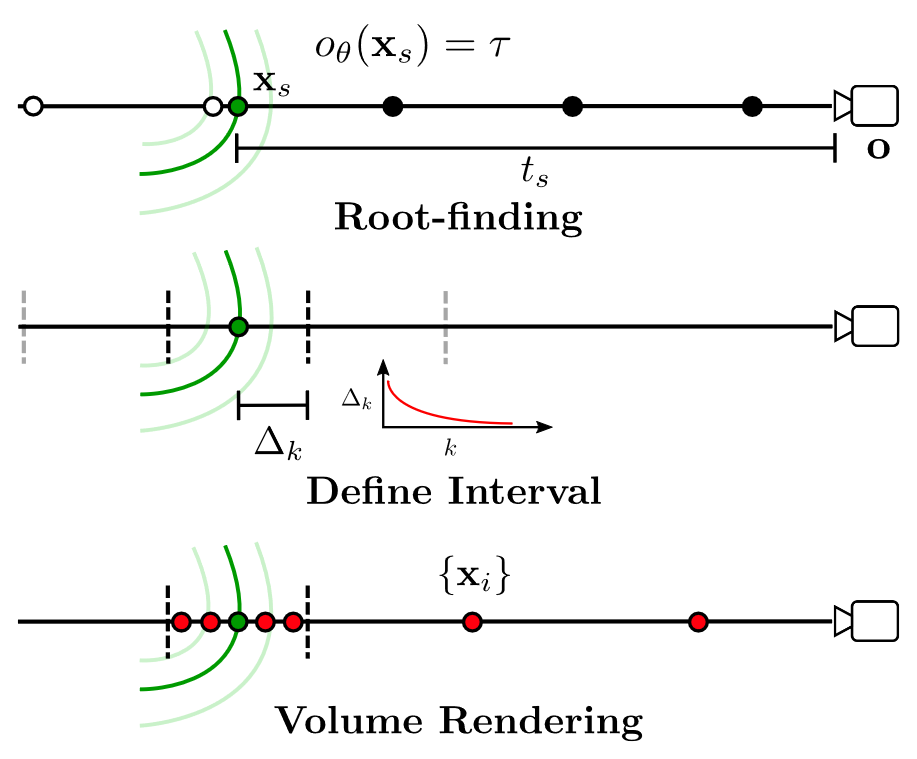
\includegraphics[width=0.8\textwidth]{undergraduate-thesis/images/unisurf-sampling.png}
    \caption{UNISURF\cite{oechsle_unisurf_2021}采样策略示意图}
    \label{fig:related-work unisurf-sampling}
\end{figure}

\subsubsection{基于误差的采样}
VolSDF\cite{yariv_volume_2021}中给出了使用符号距离场估计的不透明度$\hat{O}$的估计误差的上界:
\begin{equation}
    |O(t)-\hat{O}(t)|\leq B_{\mathcal{T},\beta}
\end{equation}

其中$B_{\mathcal{T},\beta}<\varepsilon$存在两种可能性:
\begin{enumerate}
    \item 当超参数$\beta$固定时,对于任意给定$\varepsilon$,总存在一个足够稠密的采样点集$\mathcal{T}$使得$B_{\mathcal{T},\beta}<\varepsilon$
    \item 当采样点数目$n$固定时,对于任意给定$\varepsilon$,总存在一个足够大的$\beta$使得$B_{\mathcal{T},\beta}<\varepsilon$:
    \begin{equation}
        \beta\geq\frac{\alpha t_f^2}{4(n-1)\log(1+\varepsilon)}.
        \label{eq: related-work volsdf beta-error}
    \end{equation}
\end{enumerate}

基于这一观察,VolSDF设计了一个基于误差的重采样方法:首先使用均匀采样获得初始采样点集$\mathcal{T}=\mathcal{T}_0$,通过公式\ref{eq: related-work volsdf beta-error}计算出所需要的$\beta_+$使得误差在要求范围内,接着迭代地对采样点集进行上采样,并逐步减少$\beta$直至收敛。

\begin{figure}[ht]
    \centering
    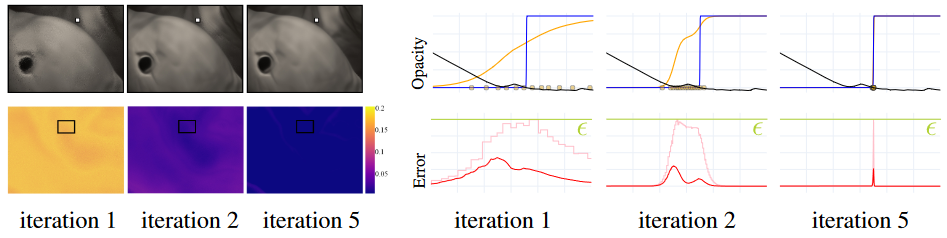
\includegraphics[width=\textwidth]{undergraduate-thesis/images/volsdf-sampling.png}
    \caption{VolSDF\cite{yariv_volume_2021}基于误差的重采样过程。}
    \label{fig:related-work volsdf-sampling}
\end{figure}

图\ref{fig:related-work volsdf-sampling}展示了VolSDF采样的迭代过程,经过数次上采样后,网络可以以很少的采样点对不透明度进行准确的估计,使得误差在要求范围内。VolSDF得到的场景几何如图\ref{fig:related-work volsdf-result}所示,由图可见VolSDF可以产生比NeRF更加准确的场景几何。

\begin{figure}[h]
    \centering
    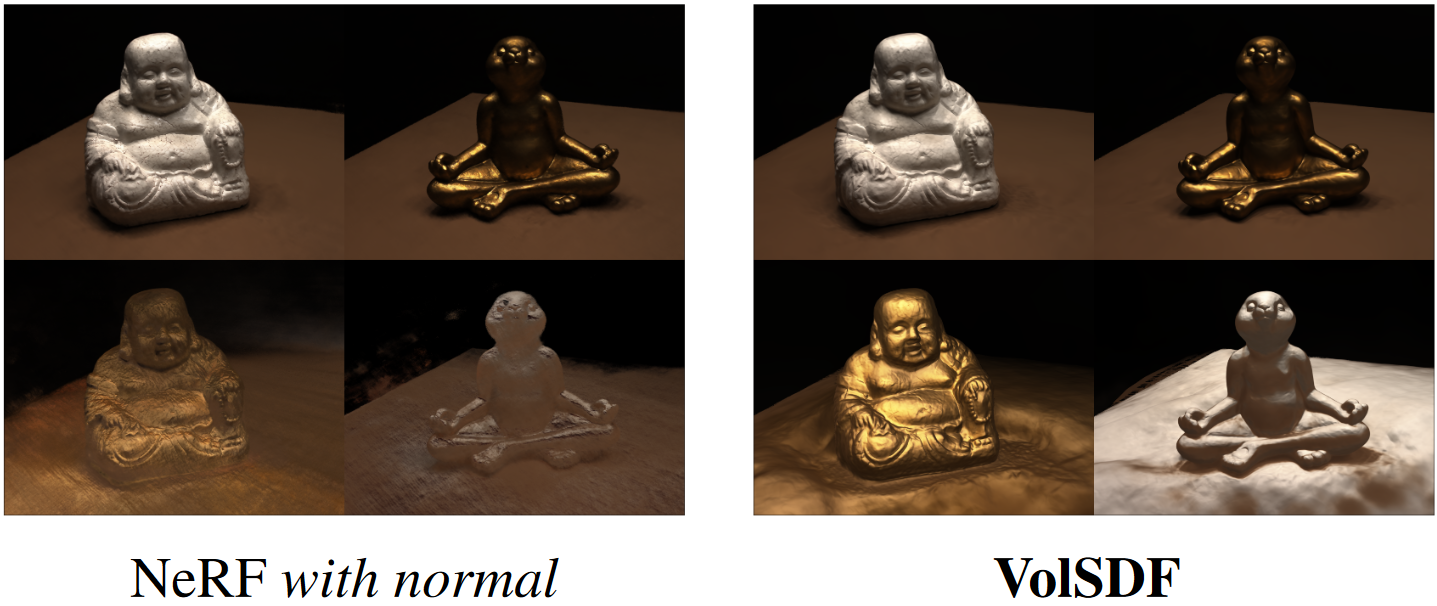
\includegraphics[width=0.7\textwidth]{undergraduate-thesis/images/volsdf-result.png}
    \caption{VolSDF\cite{yariv_volume_2021}的场景几何。}
    \label{fig:related-work volsdf-result}
\end{figure}

\subsubsection{基于Proposal网络的采样}
Mip-NeRF\cite{barron_mip-nerf_2021}使用从粗到精的重采样策略,其中 MLP 使用“粗”射线间隔评估一次,然后使用“精细”射线间隔再次评估,并在两个级别上使用图像重建损失进行监督。而Mip-NeRF 360\cite{barron_mip-nerf_2022}中则在此基础上进行了改进,使用两个MLP:一个NeRF场景表示模型,以及一个Proposal网络,其中Proposal网络根据输入空间坐标预测体密度,被用来作为重采样的基准。

\begin{figure}[ht]
    \centering
    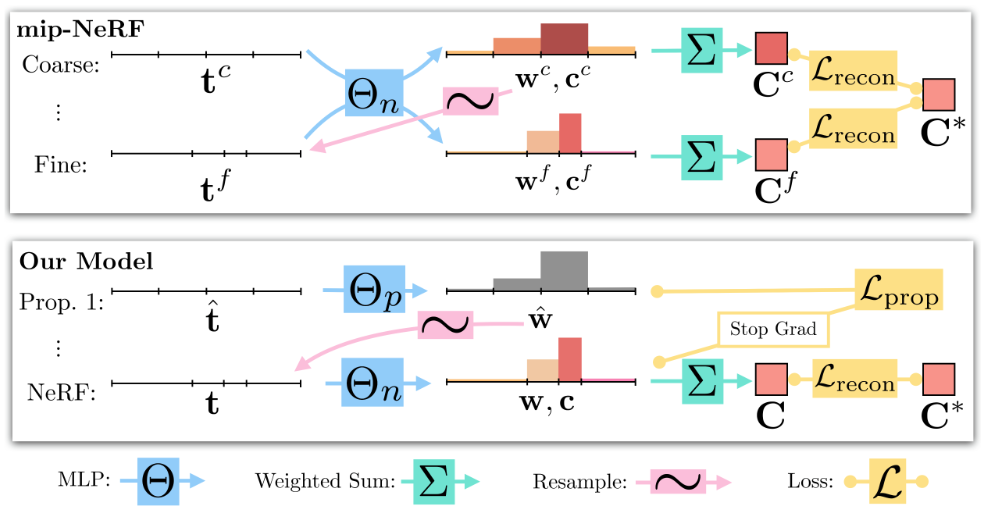
\includegraphics[width=\textwidth]{undergraduate-thesis/images/mip-nerf360 proposal network.png}
    \caption{Mip-NeRF 360\cite{barron_mip-nerf_2022} 结构示意图。}
    \label{fig:related-work proposal network}
\end{figure}

如图\ref{fig:related-work proposal network}所示,Mip-NeRF 使用一个多尺度 MLP,该 MLP 被反复查询来获取权重,这些权重被重新采样到下一阶段的间隔中,并监督在所有尺度上生成的渲染。Mip-NeRF 360使用“Proposal MLP”,在渲染阶段,使用“NeRF MLP”来生成权重和颜色来渲染图像。Proposal MLP 被训练以产生与 NeRF MLP 的 w 输出一致的Proposal权重$\hat{w}$。通过使用小型Proposal MLP 和大型 NeRF MLP,Mip-NeRF 360获得了一个具有高容量且易于训练的组合模型。

\subsubsection{基于Occupancy的网格采样}
为了提升采样效率,InstantNGP\cite{muller_instant_2022}提出使用基于占用网格的采样:当沿着光线行进进行训练和渲染时,InstantNGP希望放置样本,使它们对图像的贡献尽量均匀,从而最大限度地减少计算浪费。因此,他们通过维护一个粗略标记空与非空空间的占用网格来集中表面附近的样本。

\subsection{体渲染方法}
混合隐式场景表示中,为了同时优化符号距离场和神经辐射场,通常需要将符号距离转换成体密度来进行体积渲染,然而这一映射过程并不唯一,在这一部分中,我们介绍两种比较常见的映射。

\subsubsection{以VolSDF为代表的体渲染方法}
在体积渲染过程中,体密度$\sigma(\mathbf{x})$是一个$\mathbb{R}^3\to\mathbb{R}_+$的隐式标量函数,其值表达了光在$\mathbf{x}$点被阻挡的概率密度,也表示了该点处物体粒子的密集程度。在VolSDF\cite{yariv_volume_2021}中,作者通过一个闭式函数将符号距离值映射为体密度:
\begin{equation}
    \sigma(\mathbf{x}) = \alpha\Psi_\beta(-d_\Omega(\mathbf{x})),
    \label{eq: related-work volsdf equation}
\end{equation}
其中$\alpha,\beta$为超参数。

直观地说,体密度$\sigma$ 模拟了一个具有恒定密度$\alpha$的均匀物体,它在物体边界附近平滑减小,其中平滑程度由$\beta$控制。在式\ref{eq: related-work volsdf equation}中定义密度的好处有两方面:首先,它为表面几何形状$\mathcal{M}$提供了有用的归纳偏置,并提供了重建表面的原则性方法,即作为$\text{d}\Omega$的零值面。其次,式中定义的密度的特定形式有助于限制渲染体积的不透明度(或等效的透明度)误差,这是体积渲染管线中的一个重要组成部分。在前面的章节中,我们探讨了$\beta$的大小对于重建误差$\varepsilon$的控制作用。

\subsubsection{以NeuS为代表的体渲染方法}
然而,VolSDF所提出的经验性公式没有考虑到光线上点的先后关系,经过转换的体密度值在计算权重时也会出现偏差。NeuS\cite{wang_neus_2021}方法基于这样的观察,提出任何的转换函数$g$应满足的两个条件:
\begin{enumerate}
    \item \textbf{无偏性}:对于任意给定射线$\mathbf{r}(t)$,经由转换映射计算出的体密度通过体积渲染得到的点权重$w(t)$应在物体表面处的权重取得极大值,即在表面$t^*$($f_\text{SDF}(t^*)$)处有$\sigma'(t) = 0$;
    \item \textbf{遮挡感知}:当空间中两点$P_i$,$P_j$分别对应深度$t_i$,$t_j$满足$f_{SDF} (P_i )=f_{SDF} (P_j ),t_i<t_j$,则在渲染时须有权重$w_i>w_j$。
\end{enumerate}

\begin{figure}[ht]
    \centering
    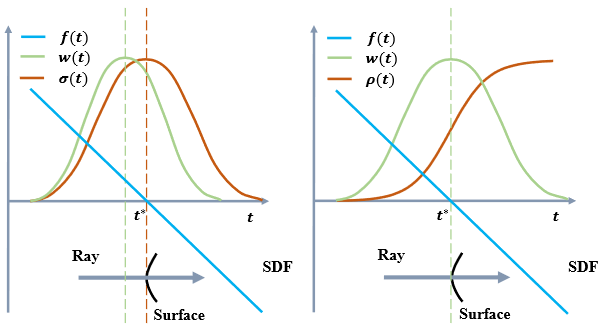
\includegraphics[width=0.9\textwidth]{undergraduate-thesis/images/neus conditions.png}
    \caption{NeuS\cite{wang_neus_2021}中提出的SDF到体密度映射函数的两个必要条件。左图所展示的传统解决方案并不能满足无偏性和遮挡感知的条件。}
    \label{fig: related-work neus conditions}
\end{figure}

如图\ref{fig: related-work neus conditions}所示,传统方法不能满足无偏和遮挡感知,因而NeuS提出了如下的转换方案:
\begin{equation}
    \sigma(t) = \max\left(\frac{-\frac{\text{d}\Phi_s}{\text{d}t}(f_{SDF}(t)}{\Phi_s(f_{SDF}(t))}, 0\right),
    \label{eq: related-work neus function}
\end{equation}
其中$\Phi_s$为Sigmoid函数的一阶导函数。

\begin{figure}[ht]
    \centering
    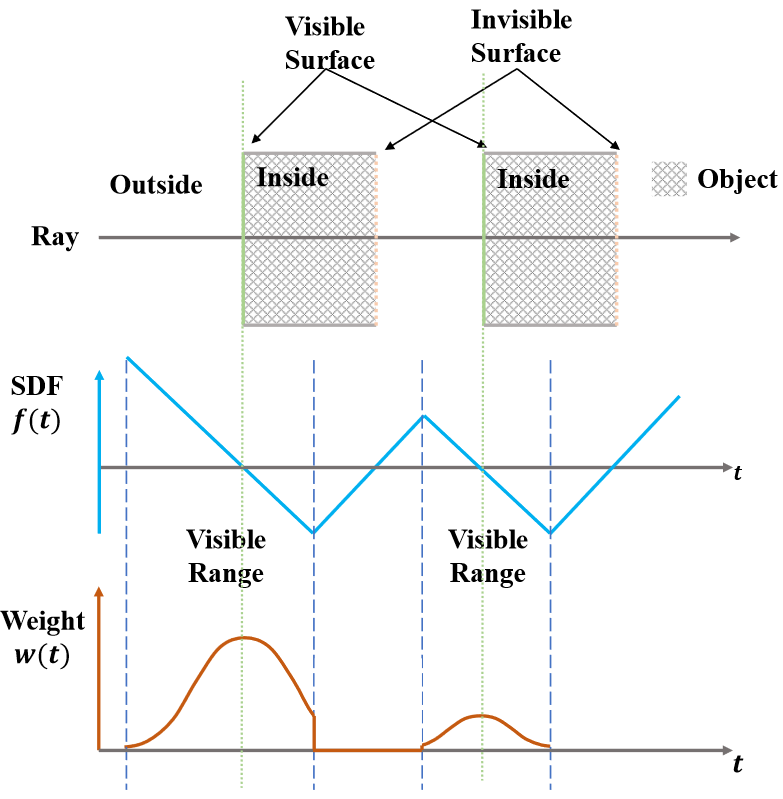
\includegraphics[width=0.8\textwidth]{undergraduate-thesis/images/neus multiple-surfaces.png}
    \caption{当射线和多个表面相交时,NeuS\cite{wang_neus_2021}提出的映射方案可以解决遮挡感知问题。}
    \label{fig:related-work occlusion-aware}
\end{figure}

可以证明,式\ref{eq: related-work neus function}中所示的映射函数可以满足其所提出的无偏性和遮挡感知要求。

\begin{figure}[ht]
    \centering
    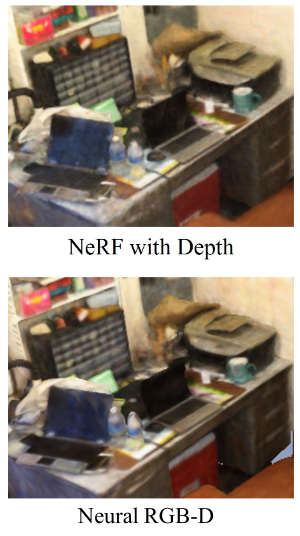
\includegraphics[width=0.5\textwidth]{undergraduate-thesis/images/neural-rgbd comparison with NeRF.png}
    \caption{直接将NeRF方法添加深度监督损失函数不能解决形状-辐射二义性。}
    \label{fig:related-work neural-rgbd comparison with NeRF}
\end{figure}

\subsection{多元传感信息融合}
虽然混合隐式表达在学习复杂场景信息时以及能在准确性上得到很大的提升,然而对于特征较少的墙面、纹理重复的表面,基于纯视觉的场景表示的精度仍然较差,一个直接的想法是使用深度传感器\cite{zabatani_intel_2020}引入深度输入作为额外的传感信号,然而直接在隐式场上添加深度监督信号会导致退化的结果(图\ref{fig:related-work neural-rgbd comparison with NeRF})。

NeuralRGB-D 是第一个将深度输入用于混合隐式表达优化的工作\cite{azinovic_neural_2022},作者使用了一个较为简单的用于体积渲染的混合隐式场方案:
\begin{equation}
    w_i = \mathtt{sigmoid}\left(\frac{f_{TSDF}(t)}{\mathtt{trunc}}\right)\cdot\mathtt{sigmoid}\left(-\frac{f_{TSDF}(t)}{\mathtt{trunc}}\right),
\end{equation}
其中$\mathtt{trunc}$为截断距离,通过加入这一超参数,使得原有的隐式符号距离场变为了一个隐式截断符号距离场,在自由空间内的距离值被设为截断距离。

\begin{figure}[htbp]
    \centering
    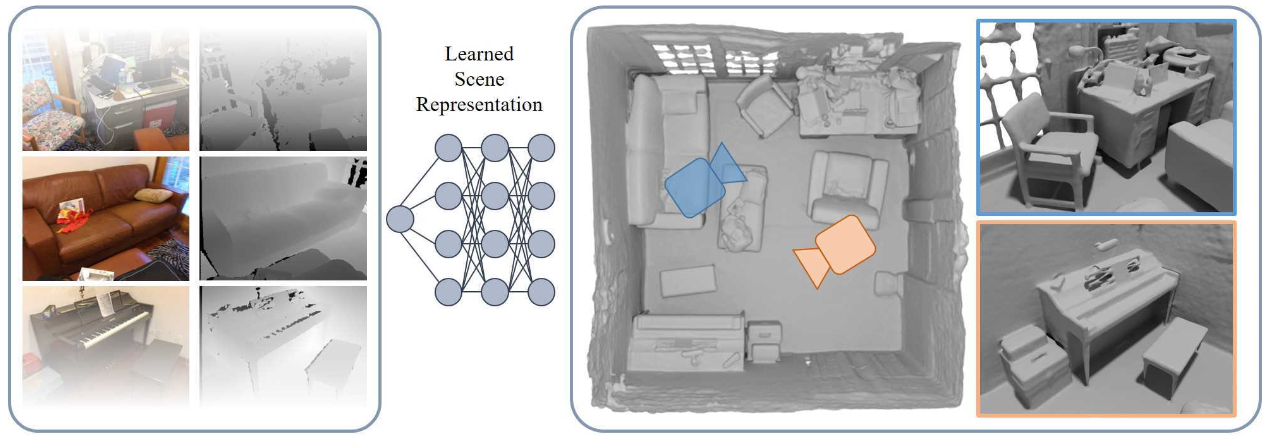
\includegraphics[width=\textwidth]{undergraduate-thesis/images/neural-rgbd problem.png}
    \caption{使用RGB-D多元信息优化隐式场的整体流程}
    \label{fig:related-work neural-rgbd formulation}
\end{figure}

我们将在下一小节中介绍该方法的优化过程。通过引入深度监督,NeuralRGB-D可以获得可信的场景表面,通过混合隐式表征的加入,减弱形状-辐射二义性对于场景表示学习的影响。

\subsection{优化混合隐式场景表示}
当只需要优化神经辐射场时,大部分方法仅使用光度误差(公式\ref{eq: related-work photometric loss})即可得到较好的优化结果,然而当我们组合不同的隐式场时,原先的单目标优化过程演变成为了一个多目标的优化过程,这对损失函数的设计带来了挑战,在本节中,我们介绍优化隐式场的几种常用损失函数。
\begin{equation}
    \mathcal{L}_{color} = \sum_r||C(r)-\hat{C}(r)||_2^2
    \label{eq: related-work photometric loss}
\end{equation}

\subsubsection{距离场优化}
注意到符号距离场编码了一个隐式表面,其梯度则代表了任意空间点到达其最近曲面的最速接近方向,因此NeuS\cite{wang_neus_2021}使用了Eikonal约束来限制距离场梯度向量趋近于单位方向向量:
\begin{equation}
    \mathcal{L}_{eikonal} = \sum_p(||\nabla f_{SDF}(p)||_2-1)^2
\end{equation}

对于截断的符号距离场\cite{azinovic_neural_2022},通常需要对场景的不同部分单独使用损失函数。在自由空间中,距离函数被截断,优化这部分距离场函数只需对网络输出的距离函数添加到截断距离$\mathtt{trunc}$的MSE损失函数:
\begin{equation}
    \mathcal{L}_{fs} = \sum_{p_{fs}}(f_{TSDF}(p_{fs})-\mathtt{trunc})^2
\end{equation}

而当空间点处于表面附近时($f_{TSDF}(p) \leq \mathtt{trunc}$)则需要根据输入深度估计该点的截断距离值,并使网络输出接近预测的截断距离:
\begin{equation}
    \mathcal{L}_{tr} = \sum_{p_{tr}}(f_{TSDF}(p_{tr})+t_{tr}-D)^2,
\end{equation}
$t_{tr}$为p点的归一化射线深度。

使用深度信息作为额外监督信号时,传统方案是直接使用网络预测深度与传感深度进行比较,使用MSE损失函数优化隐式表征:
\begin{equation}
    \mathcal{L}_{depth}=\sum_r||D(r)-\hat{D}(r)||_2^2
\end{equation}

然而由于深度传感器本身存在较大误差,直接用传感器输入值作为真实值存在一定问题,在DS-NeRF\cite{deng_depth-supervised_2022}使用KL散度使网络预测深度接近观测深度附近的一个高斯分布$\mathcal{N}(D, \hat{\sigma})$:
\begin{equation}
    \mathcal{L}_{DS-NeRF} = \sum\text{KL}[\mathcal{N}(D,\hat{\sigma}) | \hat{D}(r)]
\end{equation}

\begin{figure}[ht]
    \centering
    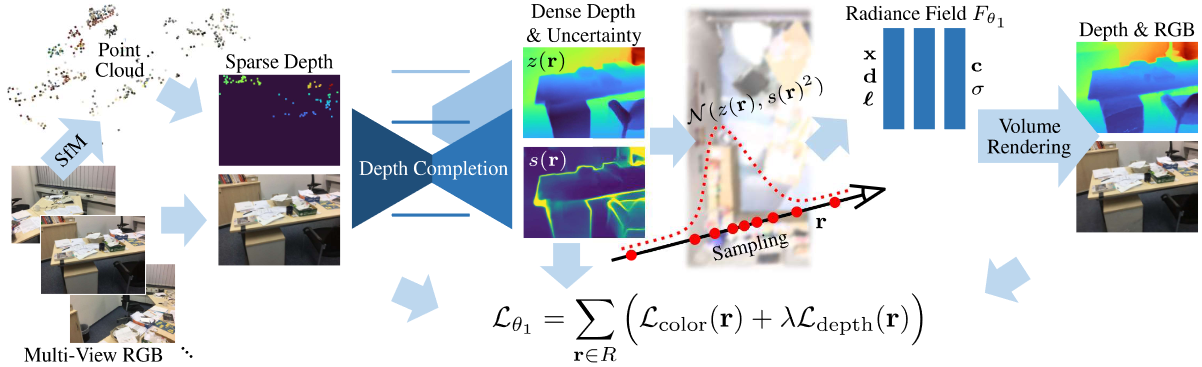
\includegraphics[width=\textwidth]{undergraduate-thesis/images/dense-depth prior.png}
    \caption{Dense Depth Prior\cite{roessle_dense_2022}中提出使用COLMAP\cite{schonberger_structure--motion_2016}稀疏点云补全后的深度作为监督信号,并引入基于不确定性的深度监督。}
    \label{fig:related-work dense depth prior}
\end{figure}

在Dense Depth Prior\cite{roessle_dense_2022}中,作者通过引入COLMAP\cite{schonberger_structure--motion_2016}稀疏点云,使用现成深度补全网络得到的深度图作为监督信号,这样生成的深度图相比深度传感器的噪声问题更加严峻,为了弥补真实深度精度的不足,作者引入了基于不确定性的深度损失函数:
\begin{equation}
    \mathcal{L}_{dense-depth}=\sum_r\left(\log(\hat{s}(r)^2)+\frac{(\hat{D}(r)-D(r))^2}{\hat{s}(r)^2}\right)
\end{equation}

\section{本章小结}
\chapter{多元传感信息神经隐式场景静态重建}
\label{chapter: omninerf}
从一系列RGB-D图片中进行三维表面重建是一个三维计算机视觉和计算机图形学中的基础研究问题。近年来,随着深度学习的发展,使用隐式方法,如神经辐射场\cite{mildenhall_nerf_2020},神经符号距离场\cite{wang_neus_2021}来重建隐式表面的方法取得了长足的进步,近期工作\cite{wang_neus_2021, azinovic_neural_2022}使用混合的辐射和距离场来共同表示场景的外观和几何信息。在本章中,我们对现有混合隐式场技术方案进行分析,提出这些方法中广泛存在的两种系统性误差, 这些误差会导致在使用深度信息作为监督信号时在重建的场景几何中的误差。在此基础之上,我们提出使用全方向距离场\cite{houchens_neuralodf_2022}代替符号距离场,并使用重新设计的优化方案对该隐式场进行优化可以在很大程度上消除这些系统误差对重建精度的影响。

除此以外,在本章中,我们还将探讨真实世界中RGB相机和深度传感器的不对齐问题。并提出使用一种新型隐式场实现RGB-D对齐的技术方案。

\section{简介}
NeRF\cite{mildenhall_nerf_2020}将一个三维场景表示为一个隐式函数(如式\ref{eq:related-work radiance field}),其输入为五维坐标$(x,y,z,\theta,\phi)$,输出为RGB色值和体积渲染密度$\sigma$。对于任意一条光线$\mathbf{r}(t) = \mathbf{o} + t\cdot\mathbf{d}$上的$N$个采样点,其空间坐标被首先输入多层感知机网络来计算体密度$\sigma$,通过继续将观察角度输入后续的全连接层,可以获得该采样点的辐射颜色值。当获得了一条射线上$N$个采样点的辐射性质,我们可以用体积渲染公式(公式\ref{eq: related-work volume rendering})获得最终渲染的像素颜色值。

然而,仅通过神经辐射场的场景体积表示存在系统性的形状-辐射二义性\cite{zhang_nerf_2020}(第\ref{sec: related-work shape-radiance ambiguity}节),不能重建高质量的几何表面,因而在导出场景网格时效果较差。为了解决这一问题,现有工作主要从两方面解决这一问题。

其中一种方式是通过修改隐式场的内在结构,引入对场景几何结构更加敏感的符号距离场作为辐射场的前置组件,使用混合隐式场来构造场景表示。将符号距离场通过抽取符号距离函数$f_{SDF}(x)$的零值面来重建隐式表面。

另一种方式则是通过引入多元传感器信息输入作为额外监督信号。现有神经辐射场方法使用图片和其相机位姿作为网络输入,使用渲染颜色和真实观测颜色作为监督信号构建损失函数。通过反向传播损失函数值来优化多层感知机网络。注意到辐射场中的体积渲染方法同样可以用来计算累计深度值,为了改善该神经网络的表示精度,现有方法通过引入深度传感信息来构建额外的监督信号\cite{deng_depth-supervised_2022, roessle_dense_2022, azinovic_neural_2022}。

虽然这两种方法在一定程度上都可以弥补形状-辐射二义性,但目前的两种技术路线都不能在更大规模场景重建准确的场景几何。本文尝试将多元传感信息,特别是深度传感数据融入重建过程。然而,简单地使用深度误差优化混合隐式场存在二义性误差。在本文中,我们首先分析将这两种技术路线相结合所带来的误差。并提出基于全方向距离场的混合隐式场景表征方法。

\section{混合隐式场内在误差}
符号距离场衡量了一个三维空间中的三维点到其最近表面的符号距离,而当符号距离函数被应用在体积渲染过程中时,通常需要显式地将距离函数值映射为体积密度或累计权重。在本文中,我们以NeuralRGB-D\cite{azinovic_neural_2022}所提出的映射方案作为示例:
\begin{equation}
    w_i = \sigma\left(\frac{f_{TSDF}(t)}{\mathtt{trunc}}\right)\cdot\sigma\left(-\frac{f_{TSDF}(t)}{\mathtt{trunc}}\right),
    \label{eq: omninerf-basedline-weighting}
\end{equation}
其中$f_{TSDF}$为神经截断符号距离函数,这个映射将符号距离函数值映射为体积积分中的点权重,$\sigma$为任意选取的钟形单峰对称函数,这里使用$\mathtt{sigmoid}$函数。这个权重分配函数在一维上的可视化如图\ref{fig:omninerf-baseline-weighting}所示。

\begin{figure}[h]
    \centering
    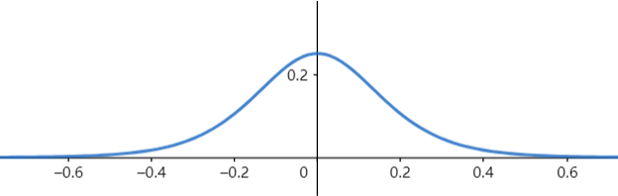
\includegraphics[width=0.6\textwidth]{undergraduate-thesis/images/neural-rgbd weighting function.png}
    \caption{公式\ref{eq: omninerf-basedline-weighting}所计算的权重函数分布。}
    \label{fig:omninerf-baseline-weighting}
\end{figure}

通过公式可以看出,距离函数较小的值将被赋予更大的体渲染权重。当距离函数通过这一函数映射到点权重后,我们可以将体积渲染公式改写为:
\begin{equation}
    \hat{C}(r) = \frac 1 {\sum_{i=0}^{N-1}w_i}\sum_{i=0}^{N-1}w_i\cdot c_i
\end{equation}

\begin{figure}[t]
    \centering
    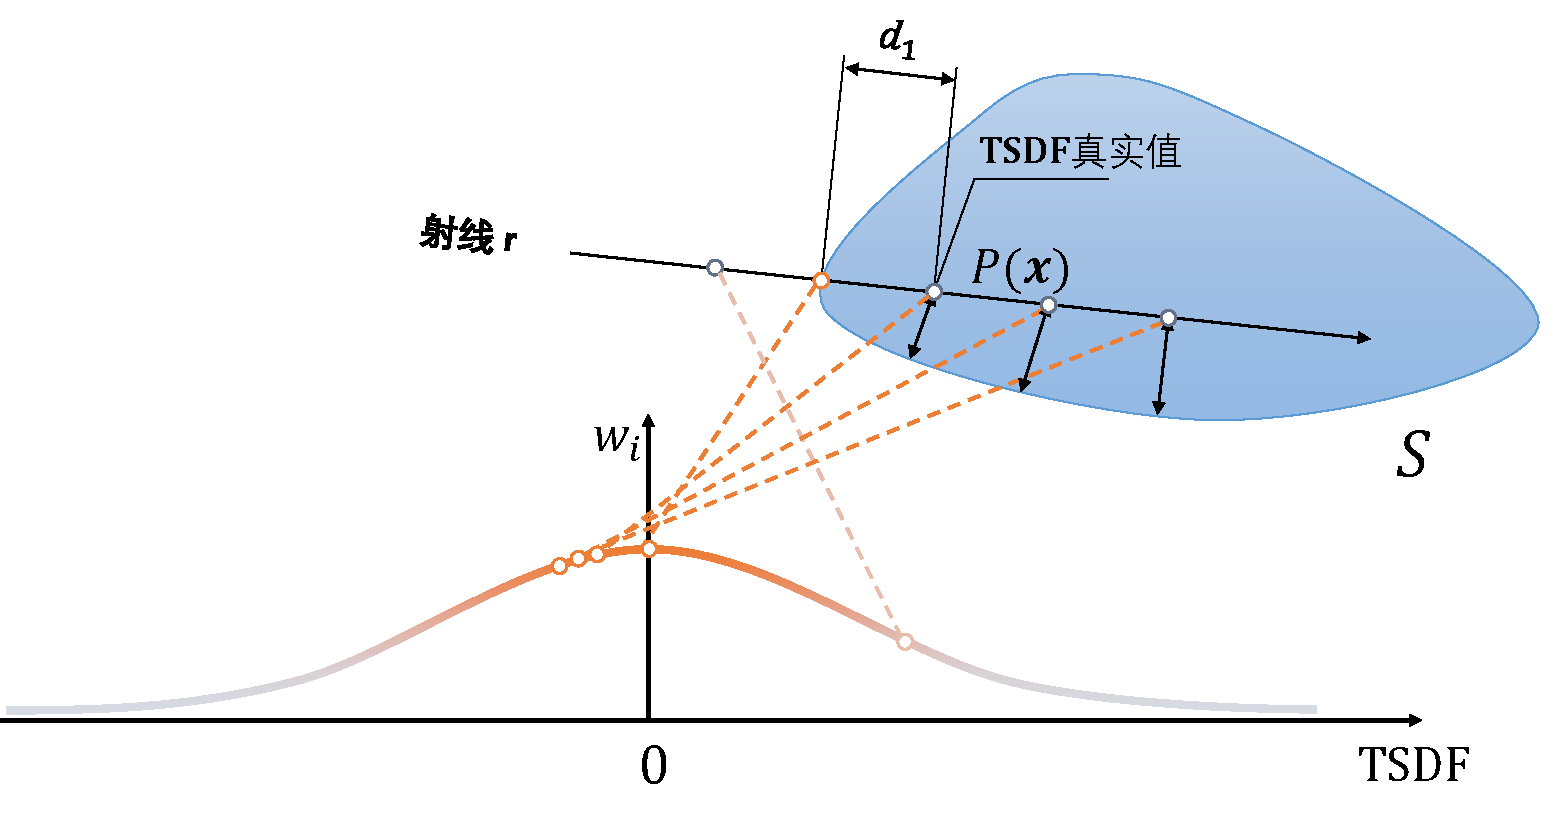
\includegraphics[width=\textwidth]{undergraduate-thesis/images/omninerf-error2.pdf}
    \caption{混合隐式场内在误差的二维示意图}
    \label{fig:omninerf-internal error}
\end{figure}

在这样的框架下, 我们描述一种由混合隐式场方案引起的系统误差。对于隐式表面$\mathcal{S}$,假设我们发射的光线$\mathbf{r}(t)$与表面$\mathcal{S}$在$t=t_0,t_1$处分布相交($t_n<t_0<t_1<t_f$),且光线$\mathbf{r}(t)$在表面$\mathcal{S}$几乎相切处入射(如图\ref{fig:omninerf-internal error}所示)。

对于$t\in[t_0, t_1]$区间中的采样点$P(t_{k_1}), \dots, (t_{k_N})$,这些点由于均位于表面$\mathcal{S}$内部,因而在体积渲染过程中,应占有较小的权重。然而,由于光线沿表面入射,当表面较为光滑时,有:
\begin{equation}
    0\approx w(t_{k_i} - t_0) << w(f_{SDF}(t_{k_i})) \approx w(0),
\end{equation}
其中$w(t_{k_i} - t_0)$较好地反映了点$t_{k_i}$处的体积,而实际预测值$w(f_{SDF}(t_{k_i}))$远远大于该点的真实密度。

由于点$t_{k_i}$靠近曲面$\mathcal{S}$表面,因而在辐射场中,该点求得的辐射颜色接近于其最近表面点$p_{k_i} + \nabla f_{TSDF}(t_{k_i})\cdot f_{TSDF}(t_{k_i})$的颜色。从而在体渲染过程中产生颜色混淆的效果。
\begin{equation}
    \hat{c}(p_{k_i})\approx\hat{c}\left(p_{k_i} + \nabla f_{TSDF}(t_{k_i})\cdot f_{TSDF}(t_{k_i})\right)
\end{equation}


\section{结合深度输入的混合隐式场距离-深度二义性}
除了前文提到的使用混合隐式场作为场景表示时出现的隐式场内在误差,我们在本节中还将介绍使用深度信号作为混合隐式场监督信号时出现的距离-深度二义性。在第二章,我们介绍了现有方法\cite{azinovic_neural_2022}在使用深度监督信号时在截断区域内所使用的深度损失函数:
\begin{equation}
    \mathcal{L}_{tr} = \sum_{p_{tr}}(f_{TSDF}(p_{tr})+t_{tr}-D)^2,
\end{equation}

该损失函数用$\hat{f}_{TSDF}(p_i) = D(\mathbf{r})-t_i$估计$p_i (p_i \in \mathbf{r})$点的截断符号距离函数。如图\ref{fig:omni-nerf depth error}所示,这个估计会对隐式场准确几何内容的学习产生很大的影响:当我们分别从两个视角$\mathbf{r}_1, \mathbf{r}_2$观察到同一空间点$P$时,由于该点到观察视角起点距离不同,由上述过程估计所得的对同一点的截断符号距离函数值$d_1, d_2$也不同,则当使用这两个不同的估计值同时作为点$P$的截断距离函数真值进行反向传播时,网络不能学到任意一个真实的TSDF值,从而导致结果模糊、计算资源浪费的结果。

\begin{figure}[ht]
    \centering
    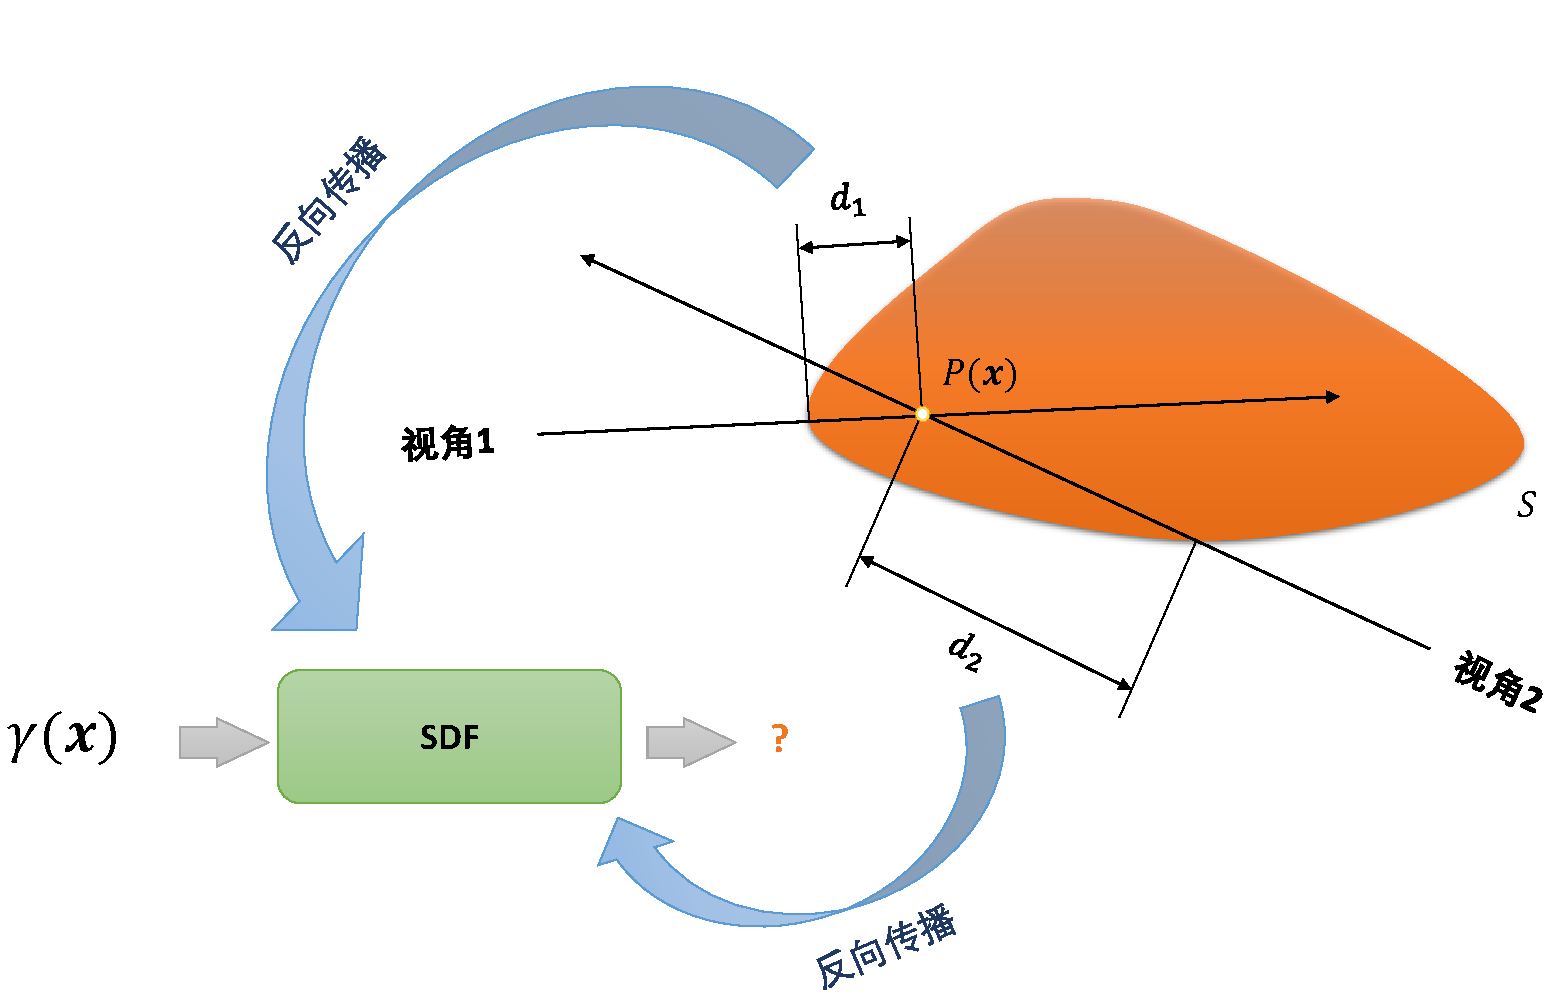
\includegraphics[width=\textwidth]{undergraduate-thesis/images/omninerf-error1.pdf}
    \caption{深度监督信号下的混合隐式场二义性示意图。}
    \label{fig:omni-nerf depth error}
\end{figure}


\section{基于全方向距离场的混合隐式场表征}
通过分析上面提到的两种误差,我们发现他们都是由于现有基于符号距离场的混合隐式表征技术方案在距离场设计上没有考虑到多视角的视角相关性,即应该使用随视角方向变化的距离函数计算权重。

基于这一观察, 在本课题中,我们提出基于全方向距离场的混合隐式表征方案。全方向距离场(Omnidirectional Distance Field, ODF)接受位置和方向的五维输入数据$(x,y,z,\theta,\phi)$,输出视角相关的距离函数值。全方向距离函数值代表了空间点$\mathbf{x}=(x,y,z)$在方向$\mathbf{d}=(\theta,\phi)$上最近表面的无符号距离。
\begin{equation}
    f_{ODF}: (\mathbf{x},\mathbf{d})\to \mathbb{R}_+
    \label{eq: omninerf-odf function}
\end{equation}

注意到全方向距离函数可以分解为符号距离场和一个全方向距离残差函数的和:
\begin{equation}
    f_{ODF}(\mathbf{x}, \mathbf{d}) = |f_{SDF}(\mathbf{x})| + f_\Delta(\mathbf{x}, \mathbf{d})
    \label{eq: omninerf-odf decomposition}
\end{equation}

我们设计了如图\ref{fig:omninerf-model}所示的网络。输入$\mathbf{x}$首先通过符号距离场得到$\mathbf{x}$的符号距离,通过将网络输出的几何参数继续前传,同时输入观察方向$\mathbf{d}$,计算空间点的全方向距离残差函数值$f_\Delta(\mathbf{x},\mathbf{d})$和辐射颜色$\mathbf{c}_i$。

\begin{figure}[ht]
    \centering
    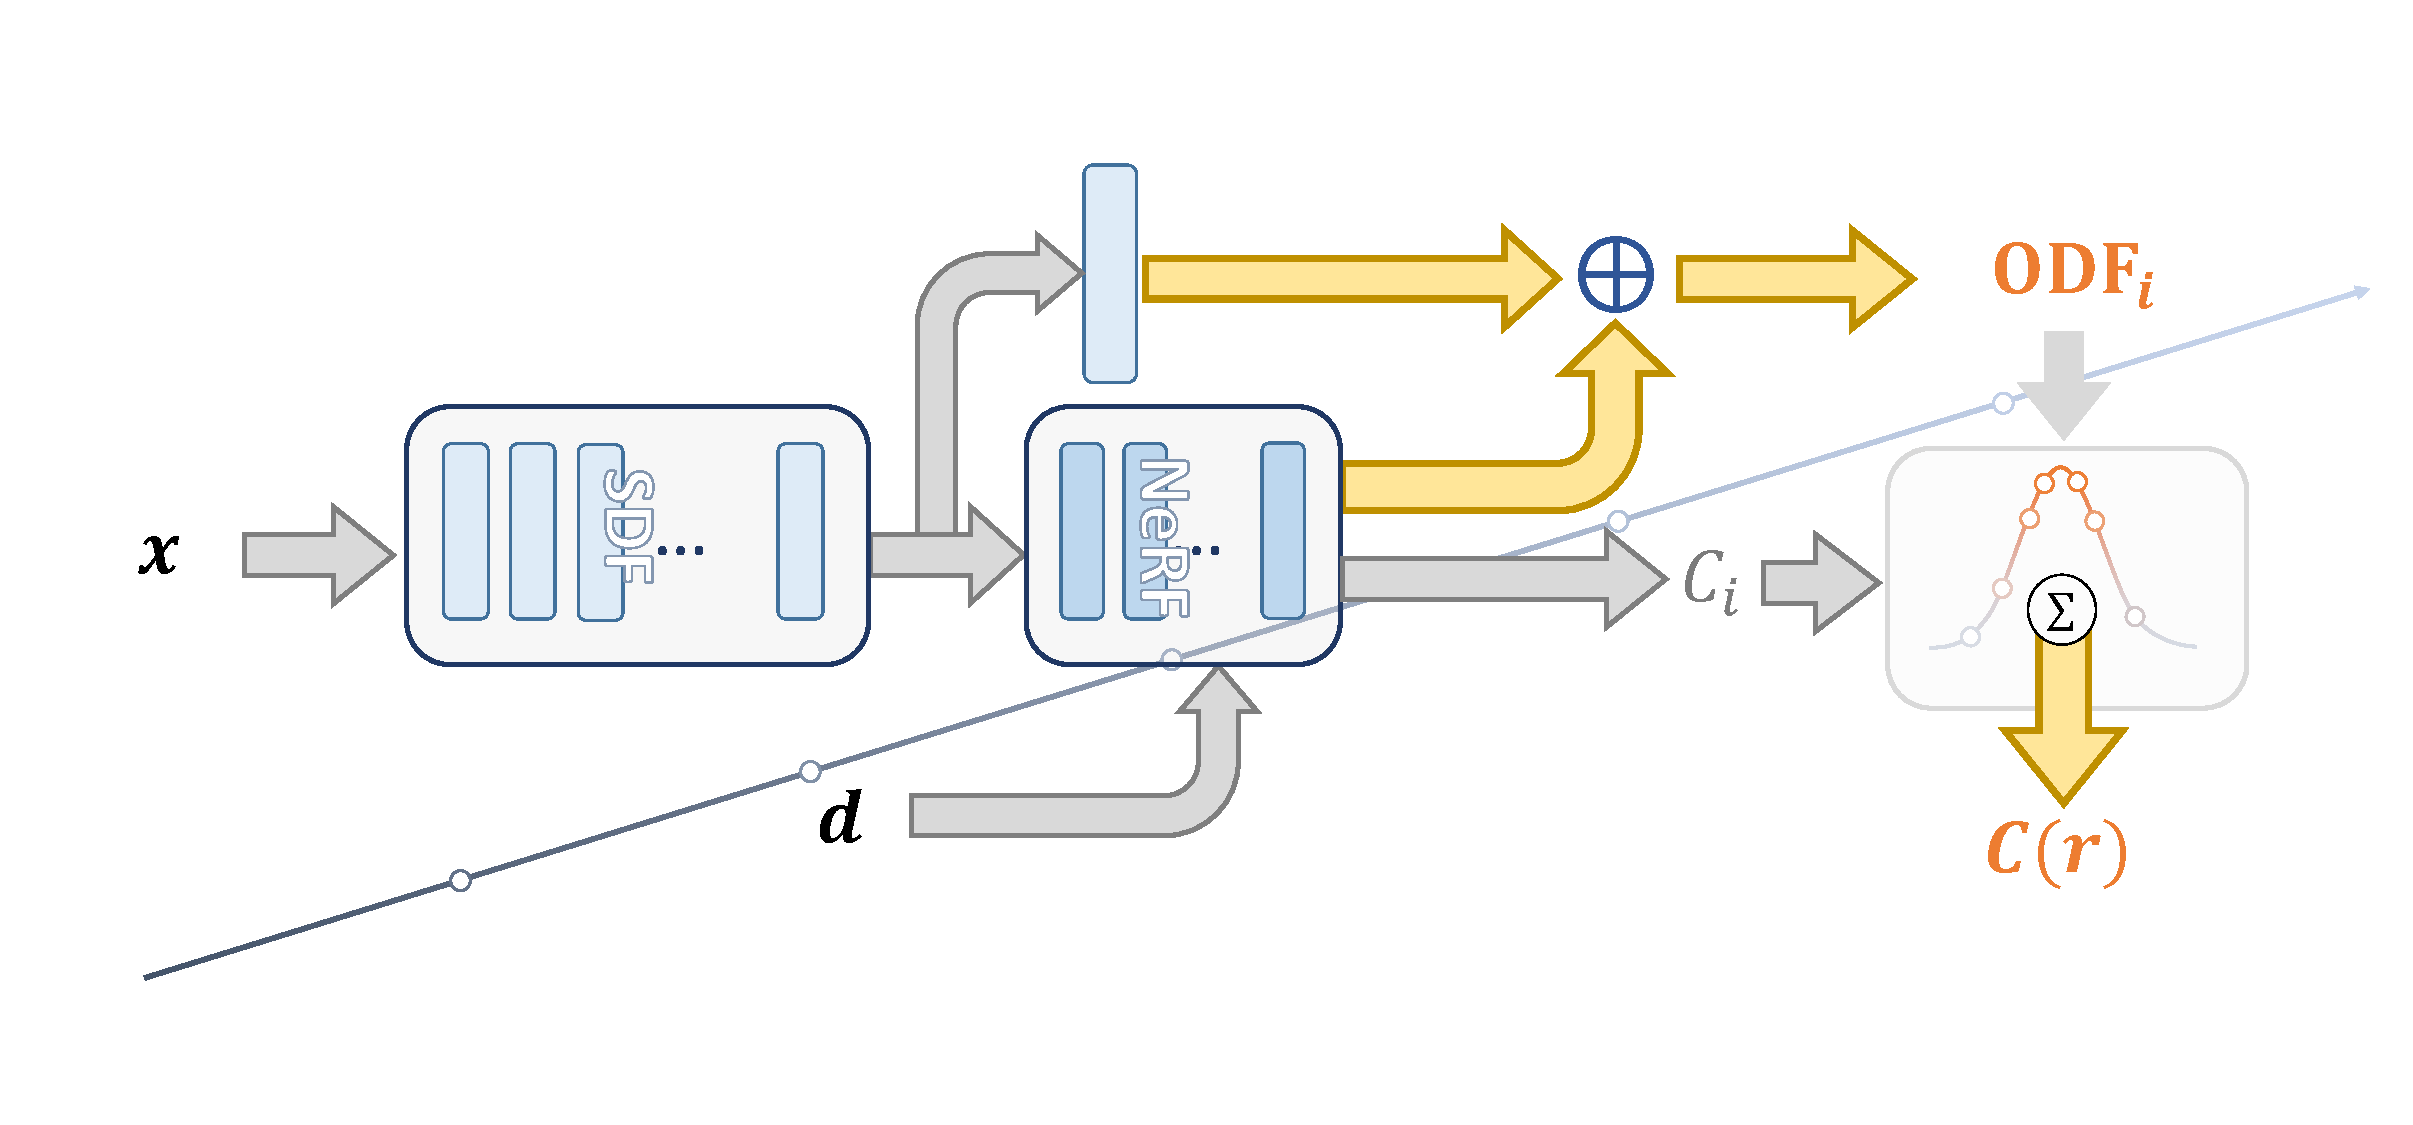
\includegraphics[width=\textwidth]{undergraduate-thesis/images/omninerf-model.pdf}
    \caption{基于全方向距离场的混合隐式表征方案}
    \label{fig:omninerf-model}
\end{figure}

通过将符号距离函数和残差函数重新组合,我们便可以得到全方向距离函数值,将该值按照现有体积渲染方案经过积分,便可以在一条射线上得到渲染颜色$C(\mathbf{r})$。 可以验证,我们提出的混合隐式场融合方案可以从理论上解决混合隐式场的内在误差和深度监督后的距离-深度二义性。

\section{场景表示实现}
在前面几节中,我们基于两种现有方法中观察到的误差和二义性,在理论上提出了可以去除这两种误差的解决方案,在本节中,我们详细描述使用全方向距离-辐射混合隐式场的实现方案。

我们在第\ref{chapter:related-work}章中介绍了现有的主流场景表示方法,其中,基于哈希体素网格的场景表示可以准确地建模场景细节但需要占据较大的存储空间,而基于多平面的张量分解场景表示在准确性上有所下降,但可以用更低的存储空间达到相媲美的效果。在本课题中,我们结合这两种不同的场景表示,使用一个较低分辨率的哈希体素网格建模场景细节,并使用一个更高分辨率的多平面作为辅助,以达到高效的准确场景地图骨干模型。我们的网络结构图如图\ref{fig:omninerf-scene-representation}所示。

\begin{figure}[ht]
    \centering
    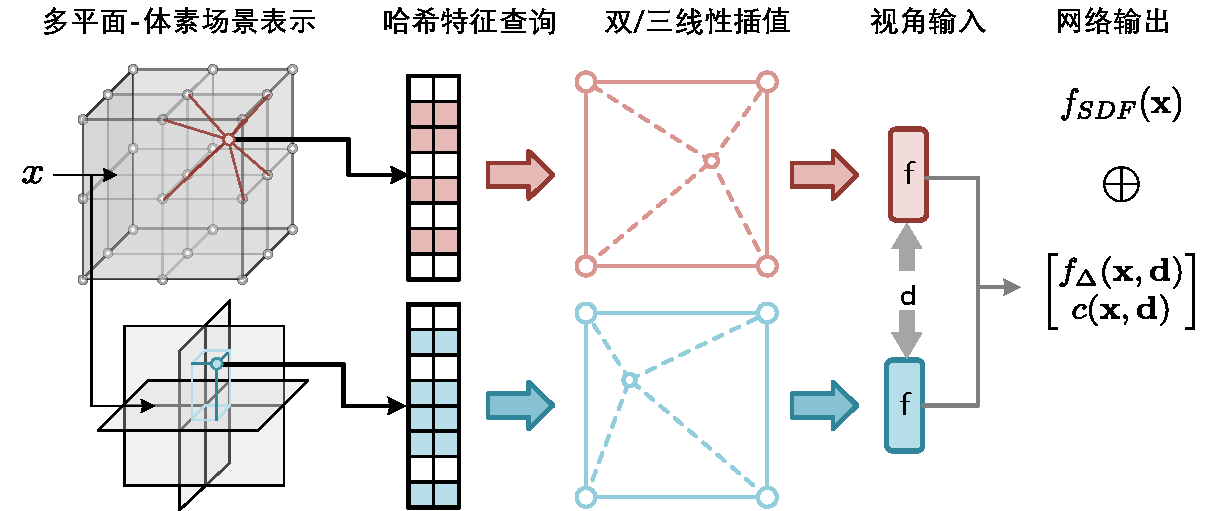
\includegraphics[width=\textwidth]{undergraduate-thesis/images/omninerf-scene-representation.pdf}
    \caption{场景表示模型架构图}
    \label{fig:omninerf-scene-representation}
\end{figure}

对于任意输入三维点$\mathbf{x}$和观察视角$\mathbf{d}$,我们分别将三维点坐标输入多分辨率体素哈希网格$\{\mathcal{G}_l\}^L$和三平面$\mathcal{P}_{\{XY,XZ,YZ\}}$。

对于多分辨率体素哈希网格,我们通过在每一分辨率级别查询输点$\mathbf{x}$的八个相邻格点,将格点序号对应哈希函数(式\ref{eq: omninerf-hash functions})作为索引,获得每个格点对应的体素特征向量。通过三线性插值$\mathtt{interp}$在连续欧式空间下获得空间点$\mathbf{x}$处的体素特征。最后将每个分辨率层级获得的特征拼接,得到该点的输出特征向量$f_{\mathcal{G}}$。
\begin{equation}
    f_{\mathcal{G}} = \mathtt{concat}\{w_l(t)\cdot\mathtt{interp}(h^l(\mathbf{x}), \mathcal{G}_l)\}_{l=1}^L,
\end{equation}
这里$w_l$为逐层抗锯齿权重,我们将在第\ref{sec: omninerf-anti-aliasing}节描述该权重的设置。
\begin{equation}
    h^l(\mathbf{x}) = \left(\bigoplus_{i}x_i\pi_i^l\right) \text{mod} T,
    \label{eq: omninerf-hash functions}
\end{equation}
$T, \pi^l$为随机大质数。

对于三平面场景表示,我们首先将输入点$\mathbf{x}$投影到XY,XZ和YZ三个平面,接着对于每个投影坐标$\mathbf{x}_{XY},\mathbf{x}_{XZ},\mathbf{x}_{YZ}$,通过上下取整得到四个相邻格点序号,用将格点序号通过哈希函数获得的索引在哈希函数表中进行查找获得该点对应的体素特征向量,最后通过双线性插值得到分解后的三个特征向量:
\begin{equation}
    f_{plane} = \mathtt{interp}(h^{plane}(\mathbf{x}_{plane}), \mathcal{P}_{plane})
    ,plane=\{XY,XZ,YZ\}
\end{equation}

通过参数融合、拼接得到完整的特征向量。该特征向量可以被后续网络结构解码成为输出物理量:
\begin{equation}
    f(\mathbf{x}) = \mathtt{concat}\{f_{\mathcal{G}}, f_{XY}\otimes f_{XZ} \otimes f_{YZ}\},
\end{equation}
这里$\otimes$为Hadamard乘积\cite{fridovich-keil_k-planes_2023}

通过参数解码器和激活函数,我们可以获得该点的无符号距离函数值:
\begin{equation}
    |f_{SDF}(\mathbf{x})| = \mathtt{activate}(f_{SDF}(f(\mathbf{x}))),
\end{equation}
其中,激活函数$\mathtt{activate}(x)=|x|$,参数解码器$f_{SDF}$为一个浅层的多层感知机。

接下来,网络会结合观察角度$\mathbf{d}$求得残差距离$f_\Delta(\mathbf{x}, \mathbf{d})$和辐射颜色$\mathbf{c}(\mathbf{x},\mathbf{d})$:
\begin{align}
    f_\Delta(\mathbf{x}, \mathbf{d})&=f_\Delta(f(\mathbf{x}), \gamma(\mathbf{d}))\\
    \mathbf{c}(\mathbf{x},\mathbf{d}) &=f_c(f(\mathbf{x}), \gamma(\mathbf{d}))
\end{align}

基于求得的无符号距离和全方向距离残差,我们通过公式\ref{eq: omninerf-odf decomposition}获得全方向距离函数值,该函数值进而通过下式中的权重函数被转换为体渲染权重:
\begin{equation}
    w(\mathbf{x},\mathbf{d}) = \mathtt{sigmoid}\left(\frac{f_{ODF}(\mathbf{x},\mathbf{d})}{\mathtt{trunc}}\right)\cdot\mathtt{sigmoid}\left(-\frac{f_{ODF}(\mathbf{x},\mathbf{d})}{\mathtt{trunc}}\right)
\end{equation}

对于射线$\mathbf{r} = (\mathbf{o},\mathbf{d})$的采样点集合$\{P_i\}_{i=0}^{N-1}$,我们对每个点$\mathbf{x}_i=\mathbf{o}+t_i\mathbf{d}$获得其全方向距离值$\{f_{ODF}(\mathbf{x}_i,\mathbf{d})\}^N$和辐射颜色$\mathbf{c}(\mathbf{x}_i,\mathbf{d})$,通过体渲染公式求得渲染点颜色和深度:
\begin{align}
    \mathbf{C}(\mathbf{r}) &= \sum_{i=0}^{N-1}w(\mathbf{x}_i,\mathbf{d})\mathbf{c}(\mathbf{x}_i,\mathbf{d})\\
    D(\mathbf{r}) &= \sum_{i=0}^{N-1}w(\mathbf{x}_i,\mathbf{d})\cdot t_i
\end{align}

\subsection{基于Proposal网络的采样策略}
与大部分体渲染方法一样,我们在渲染过程中需要使用有限的采样对体渲染积分进行近似。在本课题中,我们使用基于Proposal网络的分层采样策略。即使用一个轻量级网络,从空间点坐标估计体密度$\hat{\sigma}(\mathbf{x})$:
\begin{equation}
    f_{Proposal}:\quad \mathbf{x}\to\hat{\sigma}(\mathbf{x})
\end{equation}

我们会首先进行从相机原点$t_n$到假想无穷远点$t_f$的归一化空间中均匀采样:
\begin{equation}
    s_i\sim\mathcal{U}\left[\frac{i-1}{N}, \frac{i}{N}\right],
\end{equation}
$s_i\in(0,1]$为点的归一化深度,本课题中,我们通过下面的方式计算归一化深度:
\begin{align}
    s_i&:=\frac{g(t_i)-g(t_n)}{g(t_f)-g(t_n)}\\
    t&=g^{-1}(s\cdot g(t_f) + (1-s)\cdot g(t_n))\\
    g(t)&:= 1/x
\end{align}

采样得到粗采样的$N_c$个点的点集$\{t_i^c\}_{i=1}^{N_c}$会被输入到$f_{Proposal}$网络中查询所对应的体积密度$\{\hat{\sigma}(t_i^c)\}^{N_c}$,通过体积渲染方法计算这些点的权重:
\begin{equation}
    w_i^c = \frac{T_i(1-\exp(-\hat{\sigma}(t_i^c)\delta_i^c))}{\sum_j w_j^c},
\end{equation}
其中$\delta_i^c = t_{i+1}^c - t_i^c$为采样区间长度。$w_i^c = \text{PDF}_i$可以看作为射线上点权重分布的概率密度函数。

根据算得的概率密度函数,我们可以进行基于概率分布的重新采样,即在更高权重的地方放置更多采样点。我们首先计算累计分布值:
\begin{equation}
    \text{CDF}_i = \sum_{j \leq i} \text{PDF}_i
\end{equation}

通过在累计分布函数的逆函数$\text{CDF}^{-1}$上进行均匀采样,我们即可获得重新采样后的$N_f$个精采样点$\{t_i^f\}_{i=1}^{N_f}$,精采样点会被作为最终采样点输入到场景表达中进行体积渲染:
\begin{align}
    s^f_i &= \text{CDF}^{-1}(1/(i + 1))\\
    t^f_i &= g^{-1}(s^f_i\cdot g(t_f) + (1-s^f_i)\cdot g(t_n)
\end{align}

Proposal网络的训练需要通过从场景表达网络中蒸馏得到,注意到粗采样和精采样的采样区间并不一定相同,因而对蒸馏训练带来了一定的困难,本课题中使用覆盖损失函数的方式优化Proposal网络\cite{barron_mip-nerf_2022}。即对所有与查询区间$<t_{j}^f, t_{j+1}^f>$有交的粗采样区间,计算所有满足条件的粗采样区间权重的和。
\begin{equation}
    \mathtt{bound}(\{t_i^c\}_{i=1}^{N_c}, \{w_i^c\}_{i=1}^{N_c}, <t_{j}^f, t_{j+1}^f>) :=\sum_{k:<t_{k}^c,t_{k+1}^c>\cap<t_{j}^f, t_{j+1}^f>\neq\varnothing}\hat{w}_k^f
\end{equation}

对于任意一个精采样区间$<t_{j}^f, t_{j+1}^f>$,当满足$w_j^f\leq \mathtt{bound}(\{t_i^c\}_{i=1}^{N_c}, \{w_i^c\}_{i=1}^{N_c}, <t_{j}^f, t_{j+1}^f>)$时,则Proposal网络与场景表示网络的分布相同。因此可以利用$\mathtt{bound}$函数设计损失函数:
\begin{equation}
    \mathcal{L}_{Proposal}=\sum_j\frac{1}{w_j^f}\max(0, w_j^f- \mathtt{bound}(\{t_i^c\}_{i=1}^{N_c}, \{w_i^c\}_{i=1}^{N_c}, <t_{j}^f, t_{j+1}^f>))^2
\end{equation}

\subsection{优化全方向距离-辐射隐式场}
为了优化我们的全方向距离-辐射混合隐式场,我们设计了如下的损失函数:
\begin{equation}
    \mathcal{L} = \lambda_{color}\mathcal{L}_{color} + \lambda_{depth}\mathcal{L}_{depth}+\lambda_{ODF}\mathcal{L}_{ODF}+\lambda_{Proposal}\mathcal{L}_{Proposal},
\end{equation}
其中$\lambda_{\Box}$为对应损失函数项的权重。

在渲染颜色、深度的损失函数设计上,我们沿用现有方法\cite{mildenhall_nerf_2020}中较为常用的光度和深度误差:
\begin{align}
    \mathcal{L}_{color} &= \sum_{\mathbf{r}}||\hat{C}(\mathbf{r}) - C(\mathbf{r})||_2^2\\
    \mathcal{L}_{depth} &= \sum_{\mathbf{r}}||\hat{D}(\mathbf{r}) - D(\mathbf{r})||_2^2
\end{align}

对于全方向距离场,我们从输入深度图中估计采样点全方向距离函数值,并使用Eikonal约束\cite{gropp_implicit_2020}共同组成损失函数:
\begin{align}
    \mathcal{L}_{ODF} &= \sum_{\mathbf{r}}\sum_{i=1}^{N_f}||f_{ODF}(\mathbf{x}_i^f, \mathbf{d}) - \text{ODF}_i^{\mathbf{r}}||_2^2 + (||\nabla f_{ODF}(\mathbf{x}_i^f, \mathbf{d})||_2-1)^2\\
    \text{ODF}_i^{\mathbf{r}} &= |D(\mathbf{r}) - t_i^f|
\end{align}

\section{基于网格场景表示的抗锯齿渲染}
\label{sec: omninerf-anti-aliasing}
在第\ref{chapter:related-work}章,我们介绍了使用集成位置编码的抗锯齿渲染方法\cite{barron_mip-nerf_2021, barron_mip-nerf_2022},然而对于体素网格、多平面的场景表示,位置编码、集成位置编码均不再适用:由于PE/IPE的输出维度$2L+1$($L>5$)较高,如果构造一个高维的体素网格(即空间复杂度为$\mathcal{O}(N^{2L+1}$),将会对存储开销带来极大的负荷。

在本文中,我们利用传统计算机图形学中MipMap\cite{williams_pyramidal_1983}的思想,将其迁移在网格类场景表示中,通过设计一个新型采样点权重函数来解决锯齿问题。

在传统图形渲染管线中,当我们使用同一张高分辨率的材质图片渲染不同远近的物体时,会出现“摩尔纹”等瑕疵现象,为了解决这一问题,通常会使用MipMap的方法,即预先计算出同一物体材质贴图的不同分辨率下的一组“金字塔”。当观察物体距离相机起点较远时,使用更小分辨率的贴图进行采样,而当观察近处物体时,为了获得更多纹理细节, 则采用更大分辨率的贴图进行采样。这样做的原因是当我们从远处观察一个物体时,单个像素所覆盖的物体区域较大,此时使用高分辨率贴图进行渲染容易采样到物体表面的高频纹理细节,使用低分辨率的贴图从统计上可以理解为在像素所覆盖区域进行了超采样。

注意到多分辨率体素网格本身可以被看作场景的MipMap,为了在体素网格中模拟MipMap的效果,我们通过设计一个权重函数$w_l(t)$使距离相机较近($t\approx t_n$)使用分辨率较高的体素网格,而使较远的采样点使用分辨率较小的网格。对于$L$级多分辨率体素网格,我们通过一组一维高斯函数建模权重函数:
\begin{equation}
    w_l(t) = \mathtt{activate}(\frac{1}{\sqrt{2\pi}\sigma_l}\exp(-\frac{(t-t_l)^2}{2\sigma_l^2})),
\end{equation}
其中$\mathtt{activate}(x) = \mathtt{sigmoid}(x)$, $t_l, \sigma_l$为第$l$级体素网格所使用高斯分布的均值和标准差:
\begin{align}
    t_l &:= g^{-1}(s_l\cdot g(t_f) + (1-s_l)\cdot g(t_n)\\
    s_l &:= \frac{l + 1}{1 + L}\\
    \sigma_l &:= t_{l+1} - t_{l}
\end{align}


\section{本章小结}
\chapter{真实大规模场景数据下的混合隐式场学习}
\section{基于时间-位姿隐式场的多元传感信息配准}
大规模场景的混合隐式表达对于真实场景中地图重建是自动驾驶、无人机运输等智能交通应用的下一代地图表征工具。然而对于大规模场景的多元传感数据的同步采集,现有的同步RGB-D相机因其可以感知到的深度范围及其有限,从而不能被直接应用,而使用不同步的RGB相机和深度传感器(激光雷达等)不可避免的需要解决其中的时钟同步问题。受近期的自动标定相机内外参数的的神经隐式场方法所启发,在本节中,我们提出了首个自动标定RGB相机和深度传感器间采样频率和偏置的解决方案。

我们利用了一个重要的领域先验,即同时搭载不同种类传感器的数据采集设备在时空上覆盖了几乎完全相同的行动轨迹,提出建模时间到位姿的隐式函数关系。我们的方法可以作为第\ref{chapter: omninerf}章中混合隐式场景表示模型的前置网络,提供较为准确的位姿数据。

\subsection{简介}
近年来,神经隐式表达被广泛用于大规模场景的隐式重建中\cite{tancik_block-nerf_2022, rematas_urban_2022, turki_mega-nerf_2022, xiangli_bungeenerf_2022},由于此类方法通常具有较好的新视角渲染能力,他们通常被看作下一代视觉导航系统中的地图表示模型。我们不妨想象,在未来,同时定位与建图(Simultaneously Localization and Mapping, SLAM)系统可以快速整合不同种类的传感信息,构建准确的基于神经隐式场的地图表示\cite{zhu_nice-slam_2022, zhu_nicer-slam_2023, sandstrom_point-slam_2023},场景图(SceneGraph)算法可以通过车端RGB相机和消费级激光雷达快速构建周边区域的动态场景图,准确对路端中行人、机动车的未来轨迹进行预测\cite{ost_neural_2021, kundu_panoptic_2022, yang_urbangiraffe_2023, , chen_geosim_2021}。

然而,目前的这些方法仍然没有系统性地解决使用深度数据作为有效监督信号的一个关键问题。使用深度图作为监督信号加入到神经隐式表达的训练过程听起来是一个非常浅显易懂的概念,然而这一概念在真实大场景数据获取、使用上存在着相当复杂的时间同步问题。我们注意到市面上使用较为广泛的RGB-D同步相机如微软Kinect相机\cite{zhang_microsoft_2012}、英特尔RealSense相机\cite{, zabatani_intel_2020}等通常只能感知到受限范围内(通常在5米以内)的物体,从而只能用于室内场景的数据获取中,而不能用于更加广泛的室外场景自动驾驶、无人机运输等智能交通算法中。 另一方面,使用异步的 RGB 和深度传感器会带来更多的复杂性,因为这通常意味着我们需要估计每个RGB帧和深度帧之间的转换矩阵。

\begin{figure}[ht]
    \centering
    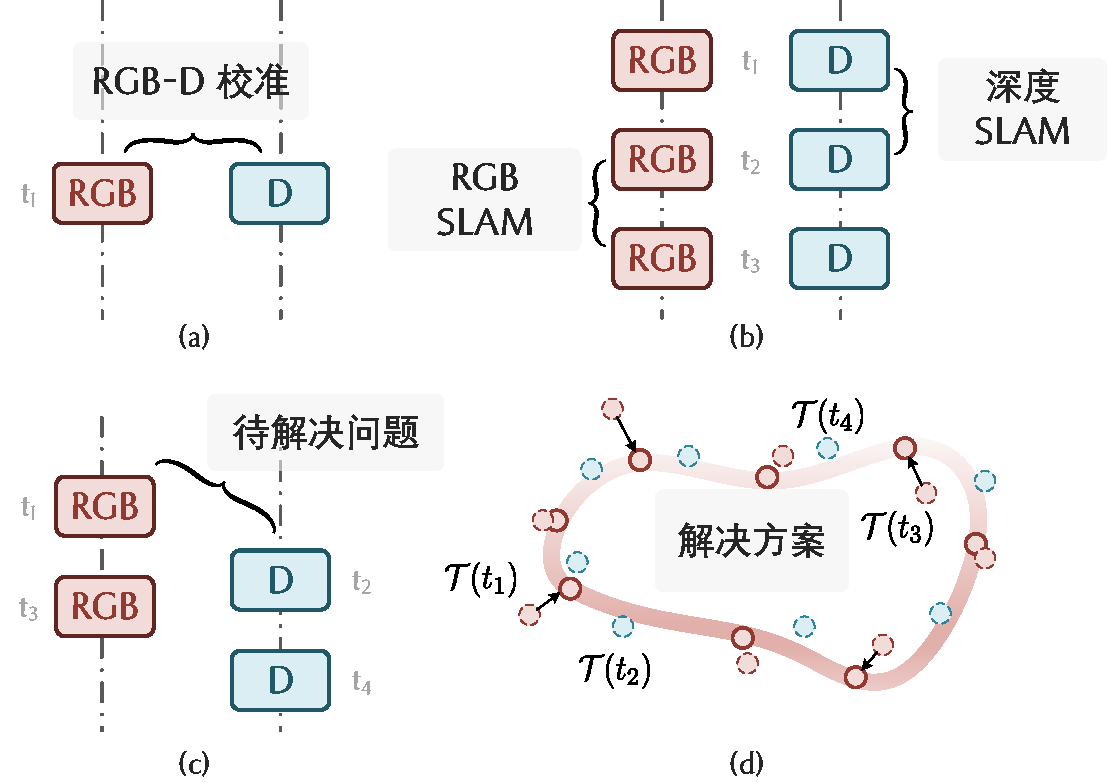
\includegraphics[width=0.8\textwidth]{undergraduate-thesis/images/time-pose function/teaser.pdf}
    \caption{我们感兴趣的问题与其他现有问题之间的比较的示意图。}
    \label{fig: time-pose function teaser}
\end{figure}

我们将我们感兴趣的问题与图\ref{fig: time-pose function teaser}中广泛关注的其他现有问题进行比较:
\begin{enumerate}
    \item [(a)]RGB-D 校准方法\cite{jeong_self-calibrating_2021, bian_nope-nerf_2022}估计深度相机和 RGB 相机之间的变换关系,即内参数矩阵,此类方法通常使用点对点的配准方法来实现;
    \item [(b)] 给定连续获取的 RGB 或深度图,基于 RGB 的 SLAM\cite{campos_orb-slam3_2021, mur-artal_orb-slam_2015, engel_direct_2018, zhu_nicer-slam_2023}和基于深度的 SLAM \cite{niesner_real-time_2013, xu_multi-scale_2018}则估计相邻帧之间的转移矩阵 $\{T_{ij}\}$;
    \item [(c)] 我们感兴趣的问题则是通过从 RGB 序列的时间戳所对应的位姿序列中,学习其中隐含的轨迹先验来估计深度序列的相机轨迹$\{T_i^d\}$。
\end{enumerate}

\begin{figure}[t]
    \centering
    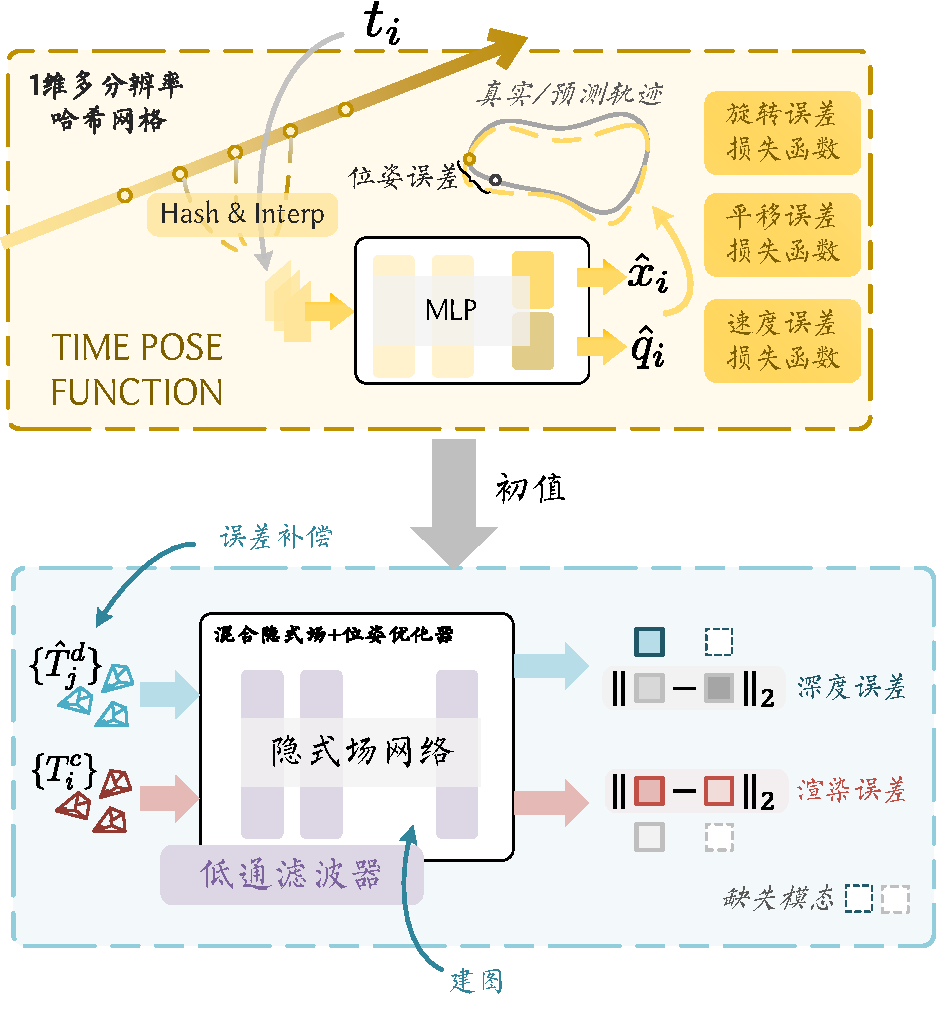
\includegraphics[width=0.8\textwidth]{undergraduate-thesis/images/time-pose function/main_export.pdf}
    \caption{系统概述图。我们的系统优化过程可以分为两个阶段。在第一阶段,TPF从 RGB 序列中时间和相机位姿之间的隐式函数关系中学习未知的深度相机位姿。在第二阶段,优化器同时训练具有深度监督的混合场景表示,并对估计的深度相机位姿进行精调。}
    \label{fig:time-pose function main figure}
\end{figure}

在本节中,我们受到近期将神经辐射场与相机内外参数同时优化的方法\cite{yen-chen_inerf_2021, lin_barf_2021, bian_nope-nerf_2022}的启发,我们希望在时空不同步的RGB-D序列中同时恢复隐式场和相机位姿的方法。我们注意到这个问题存在一个自然的解决方案:
\begin{quote}
    将 RGB 和深度帧分别处理为在某些时间戳处具有\textbf{缺失模态}的相机捕获的帧。
\end{quote}

因此,以前的方法如 BARF\cite{lin_barf_2021} 可以很容易地扩展到这种情况,即在优化开始阶段为相机内外参任意赋予一个初始值,并在优化过程中通过反向传播算法不断调整。然而,这种基线方法未能在此问题中利用有用的特定领域先验,即RGB和深度相机实际上经过相同的连续运动轨迹。

为此,我们提出使用一种新型的时间-位姿隐函数(Time-Pose Function, TPF)对此先验进行建模,TPF将时间戳映射到六自由度相机位姿。就像神经符号距离场或辐射场中对具有 3D/5D 输入的函数进行逼近的方式一样, TPF逼近一个将 1D 时间戳作为输入并输出 SE(3) 流形\cite{sola_micro_2021}中的变换的函数。换句话说,这个TPF也是一个隐式场。我们将它与前文提到的混合隐式地图结合起来,形成如图\ref{fig:time-pose function main figure} 所示的级联架构。因此,在该框架下进行优化可以同时构建用于建图的城市规模混合隐式场,并校准 RGB-D 帧之间的不匹配问题。

\subsection{相关工作概要}
\textbf{神经隐式表达:}
通过每个圆锥太体覆盖的体积的集成位置编码 (IPE) 表示,MipNeRF\cite{barron_mip-nerf_2021}有效地渲染视锥(而不是射线),从而减少了混叠的伪影现象。 NeRF++\cite{zhang_nerf_2020}分别对前景和背景表示进行建模,并分别进行采样,以应对无界 3D 场景建模的挑战。 NeRF-W\cite{martin-brualla_nerf_2021}引入了外观和瞬态编码来弥补受可变光照或瞬态遮挡物影响的弱点。 InstantNGP\cite{muller_instant_2022} 采用具有可训练特征向量的多分辨率哈希表,使 NeRF 能够学习高质量的神经图形基元。

Block-NeRF\cite{tancik_block-nerf_2022}和 Mega-NeRF\cite{turki_mega-nerf_2022} 在空间上将场景分解为单独训练的 NeRF,使场景表示能够扩展到任意大的环境。 Bungee-NeRF\cite{xiangli_bungeenerf_2022}使用多尺度数据模型,在该模型中,可以在卫星级别的截然不同的尺度上观察到图像的变化。通过引入 LiDAR 和天空建模并补偿不同的曝光,城市辐射场\cite{rematas_urban_2022}扩展了 NeRF 模型以产生令人印象深刻的 3D 表面重建并在室外环境中合成高质量的新颖视图。

此外,借助多视图立体几何\cite{deng_depth-supervised_2022} 或深度先验信息\cite{roessle_dense_2022} 的密集深度监督,NeRF 在新颖的视图合成和深度预测方面取得了惊人的成果,但难以扩展到大规模户外场景.

\textbf{相机标定:}
当前有多种 SLAM 系统通过联合估计相机参数和 3D 几何形状来重建场景。 ORB-SLAM\cite{mur-artal_orb-slam_2015}通过关联特征对应关系实时重建场景和估计相机位姿。 SfM(Structure-from-Motion,运动恢复结构) 系统\cite{schonberger_structure--motion_2016, chen_uncertainty-driven_2023} 能够同时校准内部和外部相机参数并重建场景。 相机-雷达混合SLAM\cite{kong_vmap_2023, deng_nerf-loam_2023} 对齐相机中心周围单位球体中的点和视觉特征之间的对应关系,从而提高了位姿估计精度并减少标定时间。

随着基于 NeRF 的 3D 场景重建和渲染研究的蓬勃发展,最近的工作估计了 NeRF 之上的相机参数。给定一个经过训练的 NeRF 模型,iNeRF\cite{yen-chen_inerf_2021} 能够根据观察到的图像和来自 NeRF 模型的渲染图像之间的光度损失,执行无网格、仅 RGB 的 6-DOF 位姿估计。由于 RGB 和深度的时间一致性,iMAP\cite{sucar_imap_2021} 和 NICE-SLAM\cite{zhu_nice-slam_2022} 在房间内实时进行高保真重建和位姿估计方面取得了显著成果。 Martin-Brualla 等人提出了结合 TSDF 和辐射场的混合隐式场\cite{azinovic_neural_2022},在优化相机位姿的同时提高了外观和几何形状的整体重建质量。与基于 NeRF 的方法不同,NeRFmm \cite{wang_nerf--_2022},NopeNeRF\cite{bian_nope-nerf_2022} 和 SCNeRF \cite{jeong_self-calibrating_2021} 在训练中联合优化相机位姿和内在函数。 NeRFmm\cite{wang_nerf--_2022}只能用于前向场景。 SCNeRF\cite{jeong_self-calibrating_2021} 适用于具有任意非线性失真的通用相机。两者都不能扩展到大规模场景,不适用于本文中RGB-D错配场景的设置。


\subsection{研究动机与问题描述}
问题。我们的目标是像 Mega-NeRF\cite{turki_mega-nerf_2022} 或 BungeeNeRF\cite{xiangli_bungeenerf_2022} 等先前工作中所做的那样,学习用于大规模场景表示的神经隐式场,这对于城市规划或机器人模拟等新兴应用至关重要。然而,这些先前的工作未能利用激光雷达等深度传感器捕获的几何信息。该问题现在已经收到了研究社区较大的关注\cite{deng_depth-supervised_2022,roessle_dense_2022},因为它可用于训练具有快速收敛性的无漂浮物 NeRF。为此,我们想解决在训练大规模隐式场时使用深度监督的问题。

\textbf{挑战:}
这个问题的基本挑战之一是异步 RGB-D 数据。据我们所知,没有用于大型场景的易于访问的同步 RGB-D 传感器套件(如 RealSense 或 Kinect),并且根据时间戳简单地同步它们无法完全解决错位问题。我们没有将它们与昂贵的硬件严格同步,而是从算法的角度来看。这是一个新的自校准设置:在训练大规模 NeRF 的同时在线校准 RGB-D 相机变换。

\textbf{输入:} 在使用航空图像进行大规模场景建模的许多先前工作的基础上\cite{turki_mega-nerf_2022,xiangli_bungeenerf_2022},我们假设无人机捕获的输入 RGB-D 流:一组 RGB 相机图像$\{\mathcal{I}_i\}_{i=1}^{N_c}$和一组深度图$\{\mathcal{D}_i\}_{i=1}^{N_d}$。由于异步情况存在,这两个流在概念上如图\ref{fig: time-pose function teaser}-c所示,我们的目标是恢复它们之间的时空转换。鉴于我们的重点是相对变换,在不失一般性的情况下,将 RGB 或深度的位姿作为参考点都是可行的。为方便起见,我们假设彩色图像的相机位姿是通过 SfM 算法获得的,来预测深度图位姿。

\textbf{输出}:我们的最终目标是训练一个准确的神经隐式表示,在给定的视角$\mathbf{T}$下输出逼真的 RGB 图像$\hat{\mathcal{I}}$以及准确的深度图 $\hat{\mathcal{D}}$。同时,我们校准未知的深度相机位姿$\mathbf{T}_i^d$ 有助于引入深度监督以获得更好的场景表示。

\textbf{优化过程:}
为了利用隐式时间-位姿函数关系,我们建议使用基于回归的模型,该模型将 1D 时间戳作为输入并输出相应的 6-DOF 相机位姿。在实践中,我们使用 RGB 图像位姿来训练隐式时间位姿函数并在模型收敛后预测深度位姿。然而,时间关系本身可能无法为基于 NeRF 的神经渲染器提供足够的准确性,这需要像素级的准确性来构建逼真的场景图。因此,在第二阶段,我们在 NeRF 训练过程中同时优化最初预测的深度位姿,其中 RGB 和深度图像都用作监督信号。正如我们稍后在实验中所证明的那样,使用纯 RGB 监督优化神经辐射场足以实现照片般逼真的渲染;然而,学习到的场景几何可能无法满足真实世界的机器人应用需求。引入具有原始深度位姿对齐的深度传感监督甚至可能会损害准确性。为了利用无人机在同一轨迹上捕获 RGB 图像和深度图的先验,我们对 RGB-D 帧的时间戳$\{t_i\}_{i=1}^{N_c+N_d}$ 进行建模,并且相应的相机内在函数也取自EXIF 信息作为算法输入。

\begin{figure}[ht]
    \centering
    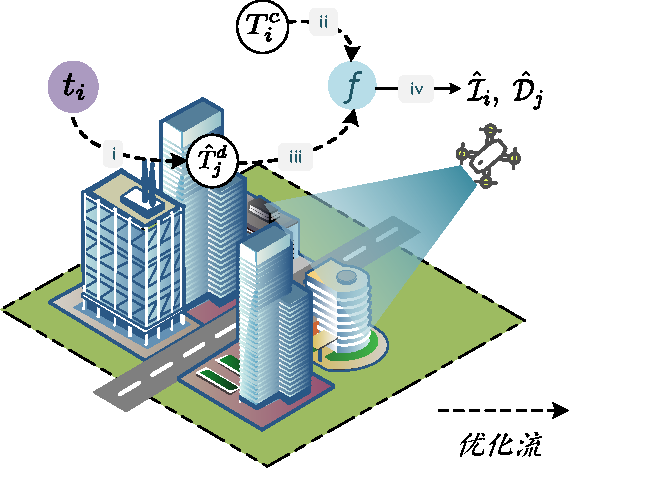
\includegraphics[width=0.6\textwidth]{undergraduate-thesis/images/time-pose function/Problem Formulation export.pdf}
    \caption{优化流程图}
    \label{fig:time-pose function optimization flow}
\end{figure}

\subsection{时间-位姿隐式轨迹函数 (TPF)}
在这一部分中,我们介绍了估计相机位姿的时间位姿函数 $\mathcal{T}$。我们将相机轨迹表示为隐式时间位姿函数,其输入是时间戳$t$,输出是 6-DoF 相机位姿。位姿输出由一个 3-D 平移向量 $x_i$ 和表示为四元数\cite{sola_micro_2021} $q_i$ 的 4-D 旋转向量组成。
\begin{equation}
    \mathcal{T}:\quad t_i\to\mathbf{T}_i=[x_i, q_i]
\end{equation}

我们将TPF函数用一个一维多分辨率哈希网格 $\{G^{(l)}\}_L^{l=1}$ 近似,输出的参数会用一个浅层多层感知机解码器$\mathcal{F}_\Theta$解码。哈希网格由 $L$ 级独立的特征网格组成。当为所有时间戳范围内的任意时间戳 $t_i$ 查询相机位姿 $\mathbf{T}_i$ 时,我们从每个网格层采样哈希编码并对提取的编码后通过二次插值并连接在一起以获得特征向量 $\mathcal{V}_i$。获得内插特征向量后,使用共享 MLP 处理特征 $\mathcal{V}_i$,然后将其输出馈送到两个分离的全连接层,以分别预测输出平移 $x_i$ 和旋转 $q_i$ 向量。网络前传过程可以用以下等式表示:
\begin{align}
    \mathcal{V}_i&=\mathcal{F}_\Theta(\mathtt{concat}\{\mathtt{interp}(h(t_i;\pi_l), \mathcal{G}_\theta^l)\}^L_{l=1}),\\
    \hat{\mathbf{T}}_i &= [\hat{x}_i, \hat{q}_i] = l_{trans}(\mathcal{V}_i; \Theta_{trans}), l_{rot}(\mathcal{V}_i; \Theta_{rot}),
\end{align}
其中$\mathtt{interp}$表示插值算子,$h$是由$π_l$参数化的哈希函数,$l_{trans},l_{rot}$是两个全连接层,其中$\Theta_{trans},\Theta_{rot}$分别表示网络参数。

由于深度图和 RGB 图像都是由同一架无人机在同一飞行中收集的,因此除了两个传感器在飞机上的位置不同外,它们在时间和空间方面的轨迹几乎相同。因此,我们可以使用我们从 RGB 序列中学习到的隐式时间-位姿函数直接预测对应于深度序列时间戳的位姿,以及传感器位置之间已知的位姿变换 $\mathbf{T}_\text{sensor}$。


\subsection{优化TPF模型}
表示用于优化相机位姿的旋转的最常见选择是旋转矩阵\cite{yen-chen_inerf_2021}或 欧拉角。然而,由于它们与 SO(3) 的非同胚表示空间,它们在表示旋转时不是连续的\cite{kendall_posenet_2015}。我们选择使用单位四元数作为我们的原始表示,因为任意 4-D 向量可以通过将它们归一化为单位长度轻松映射到合法的旋转。

为了优化时间-位姿函数,我们提出了以下目标函数:
\begin{equation}
    \mathcal{L} = \lambda_{trans}\mathcal{L}_{trans}+\lambda_{rot}\mathcal{L}_{rot}+\lambda_{speed}\mathcal{L}_{speed},
\end{equation}
其中,$\lambda_{trans}, \lambda_{rot}$会随着训练过程自动调整。我们将在后文介绍自适应权重。

\textbf{位移和旋转矢量的直接优化:}
我们通过评估估计相机位姿和地面实况相机位姿的均方误差 (MSE) 直接优化欧几里得空间中的平移和旋转向量:
\begin{align}
    \mathcal{L}_{trans} &= \text{MSE}(\{x_i\}, \{\hat{x}_i\})\\
    \mathcal{L}_{rot} &= \text{MSE}(\{q_i\}, \{\hat{q}_i\})
\end{align}

由于 $x$和 $q$ 的单位不同,因此比例因子 $\lambda_{trans}$ 和 $\lambda_{rot}$ 在平衡损失方面发挥了重要作用。为了防止平移和旋转在训练中相互产生负面影响并利用可能的相互促进作用,我们通过使用同方差不确定性 \cite{kendall_geometric_2017} 使加权因子可学习:\begin{equation}
    \mathcal{L}_{\sigma} = \mathcal{L}_{trans} \exp(−\hat{s}_{trans}) + \hat{s}_{trans} + \mathcal{L}_{rot} \exp( −\hat{s}_{rot}) + \hat{s}_{rot},
\end{equation}
其中 $\hat{s}$ 是可学习的,因此损失项会自动平衡。手动选择权重需要不断调整参数,但可以获得相似的性能。

\textbf{移动速度的梯度优化:}
观察到时间-位姿函数本质上是位移和角位移相对于时间的函数,我们可以使用平均线速度来监督网络输出相对于输入向量的梯度。这里平均速度是指从当前帧和相邻两个帧的地面真值相机位姿计算的平均值,而不是整个序列中的平均值。由于在无人机拍摄的场景中线速度变化较小,角速度变化相对较大,因此仅使用平均线速度来监督神经网络,而后者在我们的设置中没有受到监督:
\begin{equation}
    \mathcal{L}_{speed} = \text{MSE}(\{\frac{x_i-x_{i-1}}{t_i-t_{i-1}}\}, \{\hat{v}_i\})
\end{equation}

\subsection{后端优化与TPF误差补偿}
虽然时间-位姿函数为建图阶段提供了一个很好的深度相机位姿初始值,但在一些离群帧中仍然存在明显的错误。我们将描述如何同时执行映射和位姿优化,以补偿时间-位姿函数的误差。

对于地图表示,我们使用第\ref{chapter: omninerf}章所提出的混合隐式表达。在此基础指上,我们联合优化不准确的相机位姿和隐式映射:当优化场景表示参数 $\Theta_{Map}$ 时,估计的深度相机位姿 $\hat{\mathbf{T}}_i \in SE(3)$(其中 $t \in \mathbb{R}^3$, $q \in SO(3)$)将在流形上同时优化这些参数:
\begin{equation}
    \hat{\Theta}_{Map},\hat{\mathbf{T}} = \arg\min\mathcal{L}(\mathbf{T}, \Theta_{Map} | \mathbf{T}_0, \{\mathcal{I}_i\}, \{\mathcal{D}\}),
\end{equation}
其中 $\mathcal{L}$ 是目标函数,$\mathbf{T}_0$ 是时间-位姿函数的预测值。

为了补偿时间-位姿函数提取位姿的误差,我们通过应用一组可训练的位姿校正项进一步优化估计值。受 BARF\cite{lin_barf_2021} 的启发,在解决位置校准问题时,低频信号可以预测比高频信号更一致的位移,这很容易导致次优优化结果。传统 NeRF 渲染中的位置编码在高频细节方面显着改善了合成视图。使用可以削弱位置编码效果的低通滤波器将具有与平滑类似的效果。因此,在联合优化阶段中使用动态低通滤波器来帮助优化不准确的深度帧位姿。

\newpage
\section{退化真实输入数据下的准确场景表示学习}


受最近对从退化(例如,嘈杂或模糊)图像中学习辐射场的研究兴趣激增的启发,我们研究了从模糊图像中学习辐射场的问题。一个有趣的事实是,这个问题需要我们模拟由雾霾引起的真实漂浮物,而许多以前的方法侧重于避免不存在的漂浮物。我们首先证明,从模糊图像中学习的辐射场不能用于渲染可靠的深度,这与通过光衰减的雾度有关。为此,我们分析了学习到的密度值的分布,根据三个原则构建了一个加权函数,并证明了该函数可用于生成忠实的深度图。同时,我们引入了协方差损失,用于消除颜色衰减和视点相关辐射之间固有的歧义。最后,我们通过编辑辐射场中的漂浮物密度来开发雾度处理管道。
\chapter{复杂动态场景的仿真混合隐式场景表征学习}
\label{chapter: scene-graph}
最近的隐式神经渲染方法已经证明,通过预测仅由一组 RGB 图像监督的体积密度和颜色,可以为复杂场景学习准确的新视图合成。然而,现有方法仅限于学习将所有场景对象编码到单个神经网络中的静态场景的有效表示,并且缺乏表示动态场景和分解为单个场景对象的能力。本文提出了一种将动态场景分解为场景图的神经渲染方法。本文提出了一种学习的场景图表示,对场景中物体对象的刚体变换和场景内容(外观和几何等)分别进行编码,以高效地在新视角下和全新的物体信息(如轨迹信息、外观信息)下进行真实感的渲染。在此基础之上,本文对每一类具有共同特征的物体(如所有车辆、摩托)学习共同类别隐式表征,并为每个物体学习单独隐式编码,来加速网络的收敛性能。

\section{Real2Sim仿真场景重建}

从一组图像中进行视图合成和场景重建是计算机图形学和计算机视觉中的基本问题。研究人员投入了大量精力来增强计算机通过复制视觉内容来创建图片的能力。这为电影制作、机器人模拟、增强现实和电话会议等许多行业带来了巨大的价值。计算机图形学通过首先创建一个虚拟 3D 世界然后模仿光在世界中的传输方式以产生逼真的场景渲染来使用物理学对图像生成过程进行建模。为了产生视觉上吸引人的结果,基于物理的渲染需要大量的计算资源、昂贵的手动资产创建和物理建模。现有实时渲染引擎生成的图像仍然存在显着的真实感差距,降低了它们对机器人模拟和训练数据增强的影响。数据驱动的图像编辑方法,如图像合成等在过去几年中受到了极大的关注。他们专注于通过从大规模视觉数据训练的生成模型来加强渲染图像真实感。然而,大多数工作并不对应于底层逼真的 3D 世界,因此,生成的 2D 内容不能直接用于自动驾驶Real2Sim2Real应用。

近年来,随着隐式场方\cite{mildenhall_nerf_2020, barron_mip-nerf_2022, muller_instant_2022}的快速发展,在静态场景中进行高质量渲染已经日趋成熟,然而现有方法通常使用一个单一的场景表示网络来建模整个场景,因此只能建模单一静态场景,而无法建模场景中的动态物体。虽然有部分方法使用基于不确定性的可优化的隐式编码的方法忽略场景中的动态信息\cite{martin-brualla_nerf_2021},但是这类方法无法对动态物体进行渲染,更不用说面向Real2Sim的自动驾驶仿真。

本文提出一个用于表示复杂动态场景的隐式场景建模方法。通过将一个动态自动驾驶场景分解为背景节点和一组物体节点的有向图,分别对每个节点学习一个单独的隐式表征,本文可以实现对动态复杂场景的高质量建模,并且可以对物体运行轨迹和外观进行简单的编辑。

\begin{figure}[ht]
    \centering
    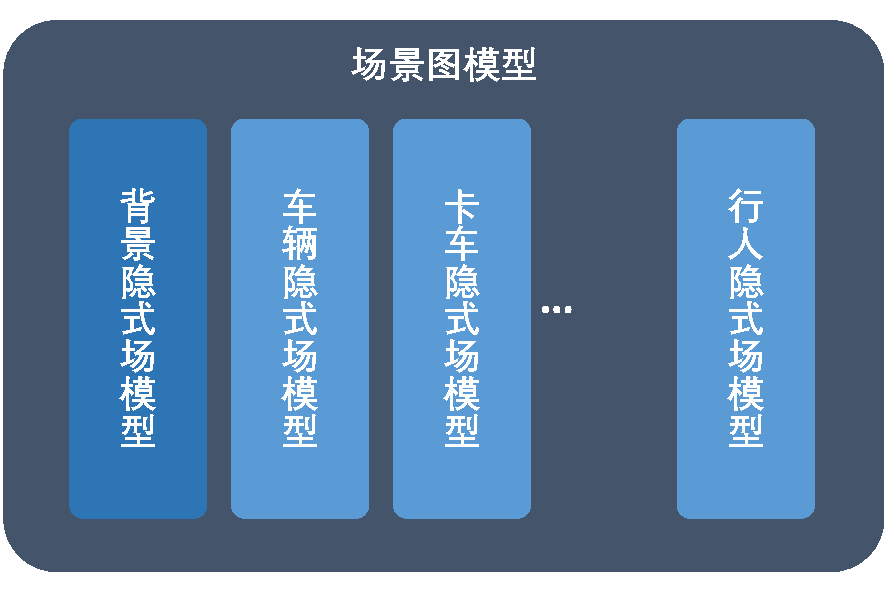
\includegraphics[width=0.6\textwidth]{undergraduate-thesis/images/related-work/scene-graph.pdf}
    \caption{场景图模型}
    \label{fig:scene-graph model}
\end{figure}

\section{基于场景图的复杂动态场景建模}

本节将介绍使用混合隐式场景图模型对复杂动态场景进行建模的方法。本文将场景图定义为一个五元组\cite{ost_neural_2021}:
\begin{equation}
    \mathcal{S} = <W, C, F, L, E>,
\end{equation}
其中,$W$为根节点,$C$为一组相机,其中主要存储相机的内参数信息,$F$为叶子节点的集合,包含背景隐式模型节点和所有物体模型节点,$L$是每类物体的可学习隐式编码,与$F$中的物体类别一一对应,$F$中的场景模型均基于本文在第\ref{chapter: omninerf}章所提出的混合隐式场景表示,$E$为在每帧中从物体节点到其对应相机节点的刚体转换矩阵,对于每个物体的三维边界框,本文用三维世界系下坐标$\mathbf{p}_o = [x, y, z]$、边界框大小尺度$s_o = [s_x, s_y, s_z]$和旋转向量$r = [r_{row}, r_{yaw}, r_{pitch}]$表示。

\begin{figure}[ht]
    \centering
    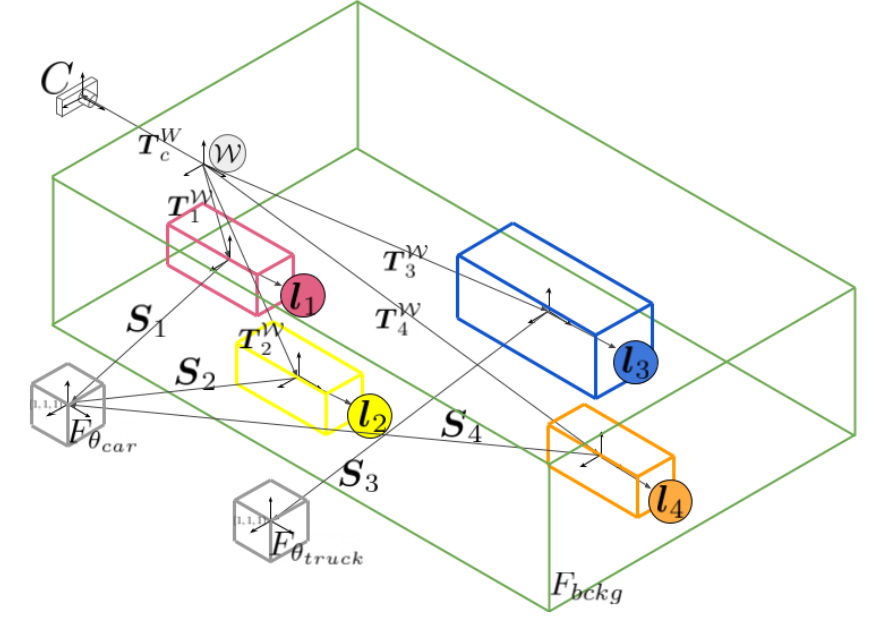
\includegraphics[width=0.8\textwidth]{undergraduate-thesis/images/related-work/nsg-scene-graph visualization.png}
    \caption{NSG\cite{ost_neural_2021}中提出的场景图分解方法。}
    \label{fig:NSG scene graph}
\end{figure}

\newcommand{\bgweight}{{\theta_{bckg}}}
\newcommand{\bgmodel}{F_{\bgweight}}
\newcommand{\classweight}{{\theta_{c}}}
\newcommand{\classmodel}{F_{\classweight}}
\newcommand{\xbf}{{\mathbf{x}}}
\newcommand{\dbf}{{\mathbf{d}}}
\newcommand{\cbf}{{\mathbf{c}}}
\newcommand{\po}{{\mathbf{p}_o}}
\newcommand{\latent}{{\mathbf{l}_o}}
\newcommand{\xo}{{\xbf_o}}
\newcommand{\dobj}{{\dbf_o}}
\newcommand{\xw}{{\xbf_w}}
\newcommand{\objpose}{\mathbf{T}_o^w}
\newcommand{\campose}{\mathbf{T}_c^w}
\newcommand{\ray}{{\mathbf{r}}}
\newcommand{\tobj}{{t_{o}}}
\newcommand{\tino}{{t_{o, in}}}
\newcommand{\touto}{{t_{o, out}}}
\newcommand{\tinw}{{t_{w, in}}}
\newcommand{\toutw}{{t_{w, out}}}

\subsection{背景节点}
对于背景建模,本文简单地直接使用此前提出的混合隐式表达作为场景模型。该模型$\bgmodel: (\xbf, \dbf) \to (\cbf, \sigma)$
将采样点的世界坐标$\xbf$和观察角度$\dbf$隐式映射到辐射颜色$\cbf$和体密度$\sigma$。

\subsection{动态物体节点}
对于动态物体,本文对第\ref{chapter: omninerf}章中的混合隐式场进行增补以使用同一个物体类别模型在同类物体中不同实例间泛化。对于每个物体,本文从其局部归一化空间中进行采样得到局部空间中的坐标$\po$,并对每个物体学习其单独的隐式编码$\latent$。因此,物体的隐式函数表达可以写作:
\begin{equation}
[\cbf(\xo), \sigma(\xo)] = \classmodel(\latent, \po, \xo, \dobj).
\end{equation}

\subsubsection{隐式物体编码学习}
为动态场景中的每个对象训练单独的场景表示很容易导致大量模型和训练工作。相反,本文的目标是最小化表示场景中所有对象的模型数量,通过学习一个类别隐式模型和若干物体隐式编码,并在渲染时将隐式编码$\latent$和物体局部坐标同时输入物体隐式表征网络,即可以达到类似使用每个物体单独网络的效果,即:
\begin{equation}
    F_{\theta_o}(\xo, \dobj) = \classmodel(\xo, \dobj, \latent).
\end{equation}

\section{复杂场景图组合渲染过程}
当物体在场景中移动时,物体边界框的世界坐标$\po$也自然会随之移动,因此本文在进行渲染的时候也需要将物体模型渲染的辐射量进行相应的移动。设物体中的一个采样点在世界系下的坐标为$\xw$,通过物体位姿的转换可以得到其在该物体的局部边界框坐标系下的坐标$\xo$:
\begin{equation}
    \xo = s_o\objpose\xw,
\end{equation}
其中$\xo\in[-1,1]$,$\objpose$是从世界坐标系到物体坐标系的位置变换。

当给定物体位姿$\{\objpose\}$和对应相机位姿时,便可以使用场景图模型进行新视角渲染。对于任意给定的一个针孔相机$C$,其内参数矩阵$K$和外参数$\campose$,可以发射一组$H\times W$的射线簇,其中每条射线可以表示为$\ray = \mathbf{o} + t\dbf$。本文在每条射线上使用基于Proposal网络的采样策略得到$N$个采样点。

为了将每个采样点分配到所应使用的模型上,本文计算射线$\ray$和物体边界框的交点。对于每条和物体边界框相较的射线, 必然存在两个采样点,这里将其进入点和射出点在世界系和物体局部坐标系下的射线深度分别写作$(\tinw, \toutw), (\tino, \touto)$。

在获得射线与物体边界框的交点后,可以将所有射线深度在这一区间中的采样点$X_o =\{\xo |\tino \leq t_{o} \leq \touto\}$分配到对应渲染模型中进行推理,其余点使用背景模型进行推理。
当所有采样点的辐射和体密度值均已求得后,可以使用体渲染方法将采样点序列渲染为输出RGB颜色。

\section{面向Real2Sim的场景图编辑}

当对一个动态场景获得其训练好的场景图后,便可以对其中的动态物体进行编辑来实现Real2Sim仿真的要求。本文在这里介绍对车辆行驶轨迹和外观进行编辑的方法。

\subsection{车辆行驶轨迹编辑}
对于场景图$\mathcal{S}$中的叶子节点$F_i$,其轨迹可以表示为时间到边界框位姿的函数:
\begin{equation}
    f_{traj}: \quad t\to<\po, s_o, r_o>.
\end{equation}

为了修改行驶轨迹,只需对位姿函数进行相应编辑,如若要使车辆在空间上按向量$\Delta\po$平移,则可生成新的轨迹为:
\begin{equation}
    f_{traj}^{trans}(t) = <\po + \Delta\po, s_o, r_o>
\end{equation}

同理,也可以对车辆进行旋转、缩放:
\begin{align}
    f_{traj}^{scale}(t) &= <\po, s_o * s', r_o>\\
    f_{traj}^{rot}(t) &= <\po, s_o, r_o + \Delta r_o>
\end{align}

通过组合上述操作,即可对车辆的行驶轨迹进行编辑。编辑效果请见实验章节。

\subsection{车辆外观编辑}
前文提到,本文对一类具有共同特征的物体使用相同的隐式表征网络,因此该网络可以在同类物体的不同实例间泛化,对于每个特定物体,只需提供一个隐式编码向量即可生成对应的物体级别网络。因此如果希望对物体形状、外观进行编辑,可以通过编辑隐式编码来实现。

对于类别网络$\classmodel$和物体隐式编码$\latent$表示的物体,若需要对该物体进行修改,一种可行的办法是在该编码上添加高斯噪声$\varepsilon\sim\mathcal{N}(0, 1)$:
\begin{equation}
    \latent' := \latent + \varepsilon
\end{equation}

这种方法可以有效改变物体外观、形状属性,但是由于高斯噪声的随机性,很难对编辑后的物体结果提前预知。为了对编辑进行控制,可以在两个同类物体的隐式编码间进行插值:
\begin{equation}
    \latent' := p\latent^{(0)} + (1 - p)\latent^{(1)}, \quad p\in[0,1]
\end{equation}

随着扩散模型\cite{ho_denoising_2020, poole_dreamfusion_2022, yang_learning_2023}的发展,通过添加和定向去除高斯噪声实现基于文本指令导向的编辑也成为可能。由于该主题与本文Real2Sim仿真场景重建的主线不符,本文不再讨论相关话题。

\section{本章小结}  
本章提出了一个基于场景图的动态复杂场景重建方法。使用视频和带标注的输入数据,本文的方法学习了多个动态和静态场景元素的连续隐式场景表示,将场景分解为多个独立的节点。本文通过使用学习的图结构在场景中生成新的对象排列来验证学习的场景图方法。这种方法还大大提高了神经渲染管道的效率,这对于从视频序列中学习至关重要。

由于该场景图分解方法是一个通用框架,而对于每个节点,其内在场景表示实现可以随意更换,因而场景图方法的迭代更新可以依靠场景表示的技术发展而实现。场景图方法目前存在的限制,如无法准确表示人体的复杂骨骼、非刚体运动等也均可以通过定制具体类别的场景表示实现。因此在未来,一个重要的发展方向是对场景图中不同类别的物体分别使用类别专属的网络结构,以适应该类物体的天然特性。

除此以外,目前的场景图方法依赖于手工的数据标注,而单目目标检测方法通常具有尺度、平移偏差,从而无法在多视角三维重建场景中被有效利用。因此一个可预见的未来发展方向是将目标检测融入场景表示中,使用端到端的场景图构建方法从只有传感器数据的数据集中学习混合隐式场景图。
\chapter{实验}

\section{数据集}
\subsection{公开数据集}
本节中介绍本文使用的公开数据集。
\subsubsection{NeuralRGB-D数据}
NeuralRGB-D\cite{azinovic_neural_2022}提出了一个基于仿真的室内场景数据集,其中包含RGB和深度的准确数据。该数据提供了在 10 个合成场景的数据集,这些场景的真实几何和相机轨迹是已知的,因此可以提供隐式场方法的定量评估指标。其中,真实相机轨迹仅用于渲染和评估,而不用于重建。对于每一帧,作者使用 Blender渲染照片般逼真的图像,其后应用噪声和伪影,来模拟类似于真实深度传感器\cite{zabatani_intel_2020, zhang_microsoft_2012}。

\begin{figure}[ht]
    \centering
    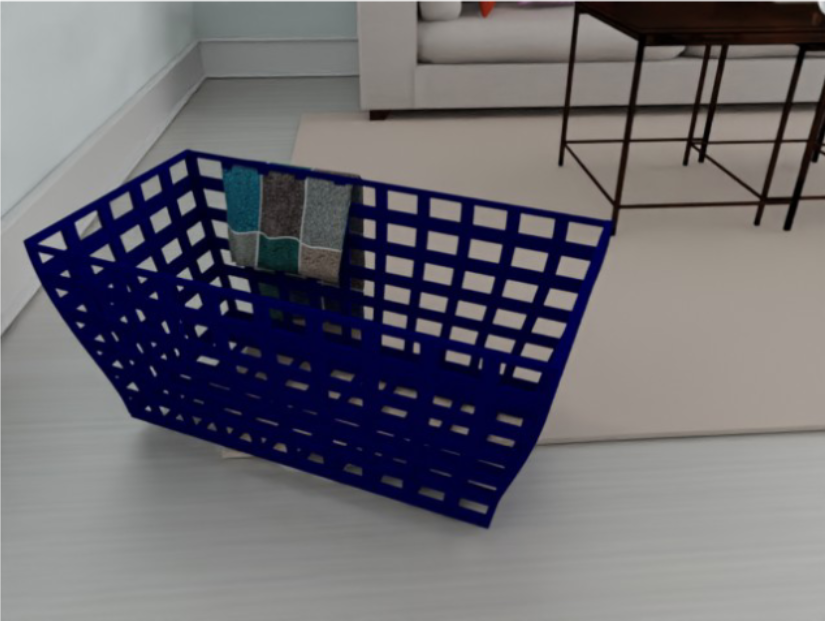
\includegraphics[width=0.6\textwidth]{undergraduate-thesis/images/experiments/neural-rgbd dataset.png}
    \caption{NeuralRGB-D\cite{azinovic_neural_2022}中的场景thin-Geometry示例图片}
    \label{fig:exp-neural-rgbd-data}
\end{figure}

\begin{figure}[ht]
    \centering
    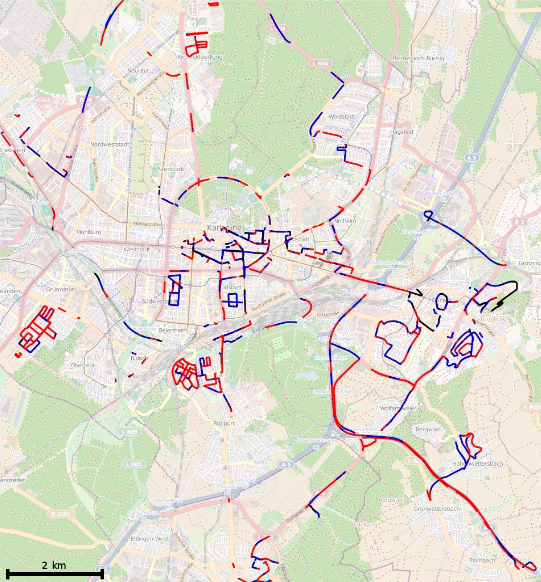
\includegraphics[width=0.8\textwidth]{undergraduate-thesis/images/experiments/kitti-map.png}
    \caption{KITTI数据集所覆盖的地图范围}
    \label{fig:exp-kitti-map}
\end{figure}

\subsubsection{KITTI数据集}
KITTI数据集\cite{geiger_are_2012,geiger_vision_2013}是是在德国卡尔斯鲁厄及其周边地区行驶时从移动平台\ref{fig:exp-kitti-platform}记录的。它包括来自组合 GPS/IMU 系统的相机图像、激光扫描、高精度 GPS 测量和 IMU 加速度。该数据集的主要目的是推动以自动驾驶为目标的计算机视觉和机器人算法的发展。在本文中,我们使用其中包含动态物体较多的片段,以验证本文所提出的场景图方法在重建复杂动态场景时的性能。
\begin{figure}[ht]
    \centering
    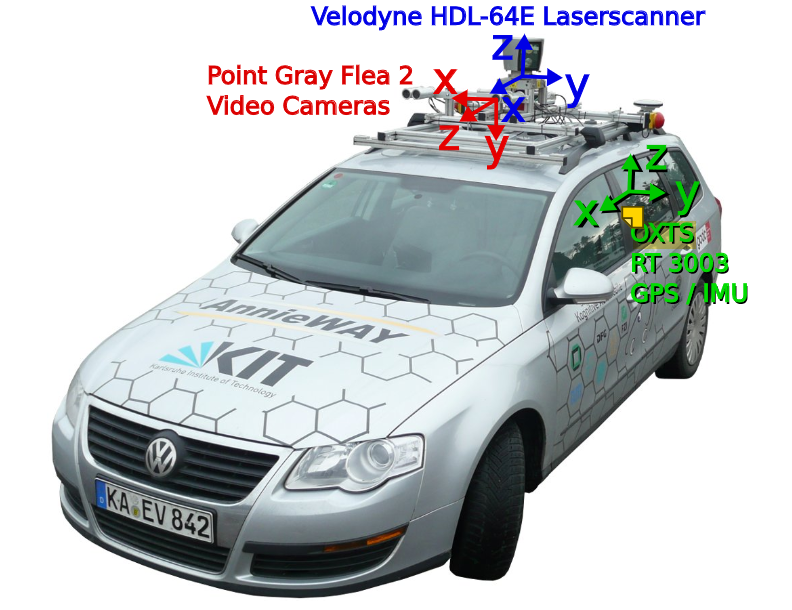
\includegraphics[width=0.8\textwidth]{undergraduate-thesis/images/experiments/kitti-platform.png}
    \caption{KITTI数据集的采集平台}
    \label{fig:exp-kitti-platform}
\end{figure}

图\ref{fig:exp-kitti-map}显示了KITTI数据集在德国卡尔斯鲁厄大都市区记录的 GPS 轨迹。颜色编码 GPS 信号质量:红色表示已使用 RTK 校正以最高精度记录,蓝色表示没有校正信号。由于没有可用的 GPS 信号,黑色部分已从数据集中排除。
KITTI数据集中提供了场景中动态物体的边界框位姿,如图\ref{fig:exp-kitti-objpose}所示。对于参考相机视野内的每个动态对象,KITTI以 3D 边界框轨迹的形式提供标注,以 Velodyne 坐标表示。数据集中定义了“汽车”、“货车”、“卡车”、“行人”、“人(坐着的)”、“骑自行车的人”、“电车”和“其他”(例如,拖车、赛格威)等多个物体类别。

\begin{figure}[ht]
    \centering
    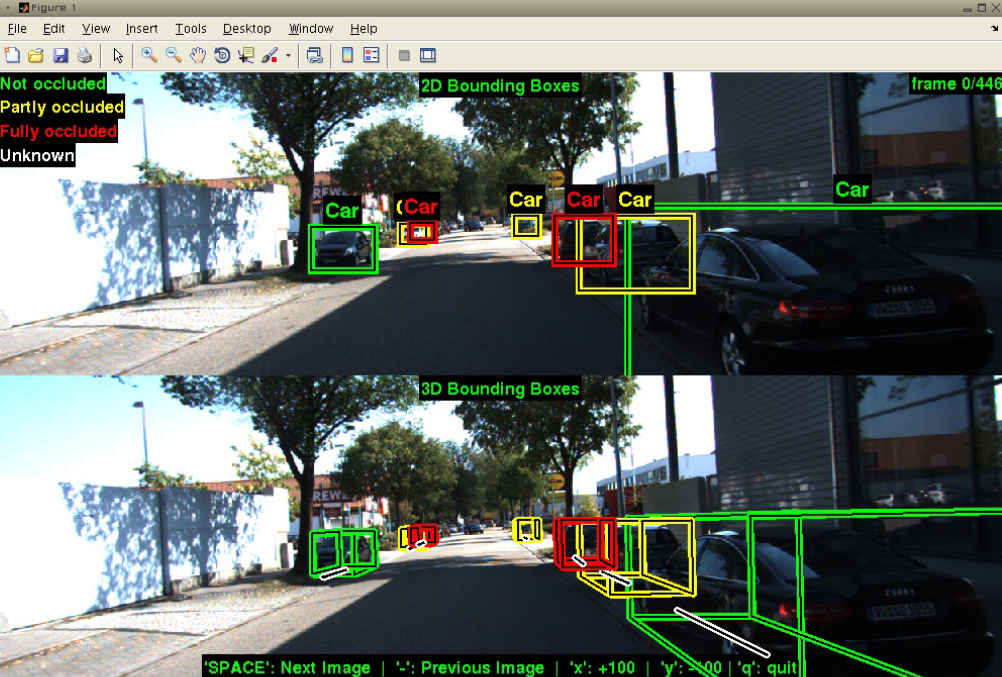
\includegraphics[width=\textwidth]{undergraduate-thesis/images/experiments/kitti-objects.png}
    \caption{KITTI中动态物体轨迹位姿标定可视化}
    \label{fig:exp-kitti-objpose}
\end{figure}



\subsection{本文提出的数据集}
\subsubsection{仿真数据集}

\subsubsection{真实数据集}

\section{混合隐式场景重建}


\section{场景图重建}

\section{体渲染方法}

\section{消融实验}

\section{本章小结}

% 后置部分
\backmatter

% 结论:在结论相应的 TeX 文件处进行结论部分的撰写
%%
% The BIThesis Template for Bachelor Graduation Thesis
%
% 北京理工大学毕业设计(论文)结论 —— 使用 XeLaTeX 编译
%
% Copyright 2020-2022 BITNP
%
% This work may be distributed and/or modified under the
% conditions of the LaTeX Project Public License, either version 1.3
% of this license or (at your option) any later version.
% The latest version of this license is in
%   http://www.latex-project.org/lppl.txt
% and version 1.3 or later is part of all distributions of LaTeX
% version 2005/12/01 or later.
%
% This work has the LPPL maintenance status `maintained'.
%
% The Current Maintainer of this work is Feng Kaiyu.
%
% Compile with: xelatex -> biber -> xelatex -> xelatex

\begin{conclusion}
  % 结论部分尽量不使用 \subsection 二级标题,只使用 \section 一级标题

  % 这里插入一个参考文献,仅作参考
  本文结论……。\cite{李成智2004飞行之梦}

  \textcolor{blue}{结论作为毕业设计(论文)正文的最后部分单独排写,但不加章号。结论是对整个论文主要结果的总结。在结论中应明确指出本研究的创新点,对其应用前景和社会、经济价值等加以预测和评价,并指出今后进一步在本研究方向进行研究工作的展望与设想。结论部分的撰写应简明扼要,突出创新性。阅后删除此段。}

  \textcolor{blue}{结论正文样式与文章正文相同:宋体、小四;行距:22 磅;间距段前段后均为 0 行。阅后删除此段。}
\end{conclusion}


% 参考文献:如无特殊需要,参考文献相应的 TeX 文件无需改动,添加参考文献请使用 BibTeX 的格式
%   添加至 misc/ref.bib 中,并在正文的相应位置使用 \cite{xxx} 的格式引用参考文献
%%
% The BIThesis Template for Bachelor Graduation Thesis
%
% 北京理工大学毕业设计(论文)参考文献 —— 使用 XeLaTeX 编译
%
% Copyright 2020-2022 BITNP
%
% This work may be distributed and/or modified under the
% conditions of the LaTeX Project Public License, either version 1.3
% of this license or (at your option) any later version.
% The latest version of this license is in
%   http://www.latex-project.org/lppl.txt
% and version 1.3 or later is part of all distributions of LaTeX
% version 2005/12/01 or later.
%
% This work has the LPPL maintenance status `maintained'.
%
% The Current Maintainer of this work is Feng Kaiyu.
%
% Compile with: xelatex -> biber -> xelatex -> xelatex
%
% 如无特殊需要,本页面无需更改

\begin{bibprint}

% -------------------------------- 示例内容(正式使用时请删除) ------------------------------------- %

% 抑制多次调用 \printbibliography 的 warning,只有示例代码会需要此语句。
% \BiblatexSplitbibDefernumbersWarningOff

% \textcolor{blue}{参考文献书写规范}

% \textcolor{blue}{参考国家标准《信息与文献参考文献著录规则》【GB/T 7714—2015】,参考文献书写规范如下:}

% \textcolor{blue}{\textbf{1. 文献类型和标识代码}}

% \textcolor{blue}{普通图书:M}\qquad\textcolor{blue}{会议录:C}\qquad\textcolor{blue}{汇编:G}\qquad\textcolor{blue}{报纸:N}

% \textcolor{blue}{期刊:J}\qquad\textcolor{blue}{学位论文:D}\qquad\textcolor{blue}{报告:R}\qquad\textcolor{blue}{标准:S}

% \textcolor{blue}{专利:P}\qquad\textcolor{blue}{数据库:DB}\qquad\textcolor{blue}{计算机程序:CP}\qquad\textcolor{blue}{电子公告:EB}

% \textcolor{blue}{档案:A}\qquad\textcolor{blue}{舆图:CM}\qquad\textcolor{blue}{数据集:DS}\qquad\textcolor{blue}{其他:Z}

% \textcolor{blue}{\textbf{2. 不同类别文献书写规范要求}}

% \textcolor{blue}{\textbf{期刊}}

% \noindent\textcolor{blue}{[序号]主要责任者. 文献题名[J]. 刊名, 出版年份, 卷号(期号): 起止页码. }

% \printbibliography [type=article,heading=none] 

% \textcolor{blue}{\textbf{普通图书}}

% \noindent\textcolor{blue}{[序号]主要责任者. 文献题名[M]. 出版地: 出版者, 出版年. 起止页码. }
% \cite{Raymer1992Aircraft}

% \printbibliography [keyword={book},heading=none] 

% \textcolor{blue}{\textbf{会议论文集}}

% \noindent\textcolor{blue}{[序号]析出责任者. 析出题名[A]. 见(英文用In): 主编. 论文集名[C]. (供选择项: 会议名, 会址, 开会年)出版地: 出版者, 出版年. 起止页码. }
% \cite{sunpinyi}

% \printbibliography [type=inproceedings,heading=none] 

% \textcolor{blue}{\textbf{专著中析出的文献}}

% \noindent\textcolor{blue}{[序号]析出责任者. 析出题名[A]. 见(英文用In): 专著责任者. 书名[M]. 出版地: 出版者, 出版年.起止页码. }
% \cite{luoyun}

% \printbibliography [type=inbook,heading=none] 

% \textcolor{blue}{\textbf{学位论文}}

% \noindent\textcolor{blue}{[序号]主要责任者. 文献题名[D]. 保存地: 保存单位, 年份. }
% \cite{zhanghesheng}
% \cite{Sobieski}

% \printbibliography [keyword={thesis},heading=none] 

% \textcolor{blue}{\textbf{报告}}

% \noindent\textcolor{blue}{[序号]主要责任者. 文献题名[R]. 报告地: 报告会主办单位, 年份. }
% \cite{fengxiqiao}
% \cite{Sobieszczanski}

% \printbibliography [keyword={techreport},heading=none] 

% \textcolor{blue}{\textbf{专利文献}}

% \noindent\textcolor{blue}{[序号]专利所有者. 专利题名[P]. 专利国别: 专利号, 发布日期. }
% \cite{jiangxizhou}

% \printbibliography [type=patent,heading=none] 

% \textcolor{blue}{\textbf{国际、国家标准}}

% \noindent\textcolor{blue}{[序号]标准代号. 标准名称[S]. 出版地: 出版者, 出版年. }
% \cite{GB/T16159—1996}

% \printbibliography [keyword={standard},heading=none] 

% \textcolor{blue}{\textbf{报纸文章}}

% \noindent\textcolor{blue}{[序号]主要责任者. 文献题名[N]. 报纸名, 出版年, 月(日): 版次. }
% \cite{xiexide}

% \printbibliography [keyword={newspaper},heading=none] 

% \textcolor{blue}{\textbf{电子文献}}

% \noindent\textcolor{blue}{[序号]主要责任者. 电子文献题名[文献类型/载体类型]. 电子文献的出版或可获得地址(电子文献地址用文字表述), 发表或更新日期/引用日期(任选). }
% \cite{yaoboyuan}

% \printbibliography [keyword={online},heading=none] 

% \textcolor{blue}{关于参考文献的未尽事项可参考国家标准《信息与文献参考文献著录规则》(GB/T 7714—2015)}

% 在使用时,请删除/注释上方示例内容,并启用下方语句以输出所有的参考文献
\printbibliography[heading=none]
\end{bibprint}

% 附录:在附录相应的 TeX 文件处进行附录部分的撰写
%%
% The BIThesis Template for Bachelor Graduation Thesis
%
% 北京理工大学毕业设计(论文)附录 —— 使用 XeLaTeX 编译
%
% Copyright 2020-2022 BITNP
%
% This work may be distributed and/or modified under the
% conditions of the LaTeX Project Public License, either version 1.3
% of this license or (at your option) any later version.
% The latest version of this license is in
%   http://www.latex-project.org/lppl.txt
% and version 1.3 or later is part of all distributions of LaTeX
% version 2005/12/01 or later.
%
% This work has the LPPL maintenance status `maintained'.
%
% The Current Maintainer of this work is Feng Kaiyu.
%
% Compile with: xelatex -> biber -> xelatex -> xelatex

\begin{appendices}
  \section{还没写完的部分备忘}
  \begin{enumerate}
      \item 第二章文献综述中RGB-D对齐的部分没写,动态部分没写。
      \item 第二章文献综述的故事逻辑需要重新梳理,目前是罗列文献的状态
      \item 第三章简介和总结没写;还可以补一个NeRF-W和Block-NeRF
      \item 第五章没写
      \item 实验没写
      \item 总结没写
      \item 致谢没写
      \item 如果有时间可以把图片都换成中文矢量图,有些图现在用的是宋体,后面同一换成等线了,不过我其实想全部换成柳楷体
      \item 可能第三章proposal network和mip with grid可以补个图
      \item related-work 图片应该拖到对应文件夹下面
      \item 附录把supp放进来
  \end{enumerate}

\end{appendices}


% 致谢:在致谢相应的 TeX 文件处进行致谢部分的撰写
%%
% The BIThesis Template for Bachelor Graduation Thesis
%
% 北京理工大学毕业设计(论文)致谢 —— 使用 XeLaTeX 编译
%
% Copyright 2020-2022 BITNP
%
% This work may be distributed and/or modified under the
% conditions of the LaTeX Project Public License, either version 1.3
% of this license or (at your option) any later version.
% The latest version of this license is in
%   http://www.latex-project.org/lppl.txt
% and version 1.3 or later is part of all distributions of LaTeX
% version 2005/12/01 or later.
%
% This work has the LPPL maintenance status `maintained'.
%
% The Current Maintainer of this work is Feng Kaiyu.
%
% Compile with: xelatex -> biber -> xelatex -> xelatex

% 致谢部分尽量不使用 \subsection 二级标题,只使用 \section 一级标题
\begin{acknowledgements}
  值此论文完成之际,首先向我的导师……

  \textcolor{blue}{致谢正文样式与文章正文相同:宋体、小四;行距:22 磅;间距段前段后均为 0 行。阅后删除此段。}
\end{acknowledgements}


\end{document}
